\clearpage
\section{الإجراءات الداخلية}
\label{sec:builder-feature-internal-sops}

صفحة «الإجراءات الداخلية» هي نقطة البداية لكل إجراء تبنيه. فهي تعرض الإجراءات الموجودة في مجلدات، وتبيّن حالة كل إجراء ونتائج عمليات تشغيله الأخيرة، ومنها تنشئ إجراءً جديداً أو تفتح إجراءً قائماً لتعديله. وتساعدك مؤشرات الصحة فيها على ملاحظة الإجراء الذي بدأ يفشل قبل أن يشتكي أحد.

\textbf{المسار ومن يستخدمه:} «ادوات البناء» ← «الأساسية» ← «الإجراءات الداخلية». يستخدمها من يصمم مسارات العمل في المؤسسة ويتابع تشغيلها.

\begin{rcnote}[مثال: شركة الأفق]
يبني مسؤول النظام إجراء «اعتماد طلب الزيارة» يبدأ «عند إرسال نموذج» طلب الزيارة، فيرسل «طلب موافقة» إلى سارة الخطيب، ثم يُنشئ لعمر حداد مهمة تجهيز الزيارة إذا وافقت. ويبدأ الإجراء من ② ويتابع عمليات تشغيله من ④.
\end{rcnote}

\begin{figure}[H]
\centering
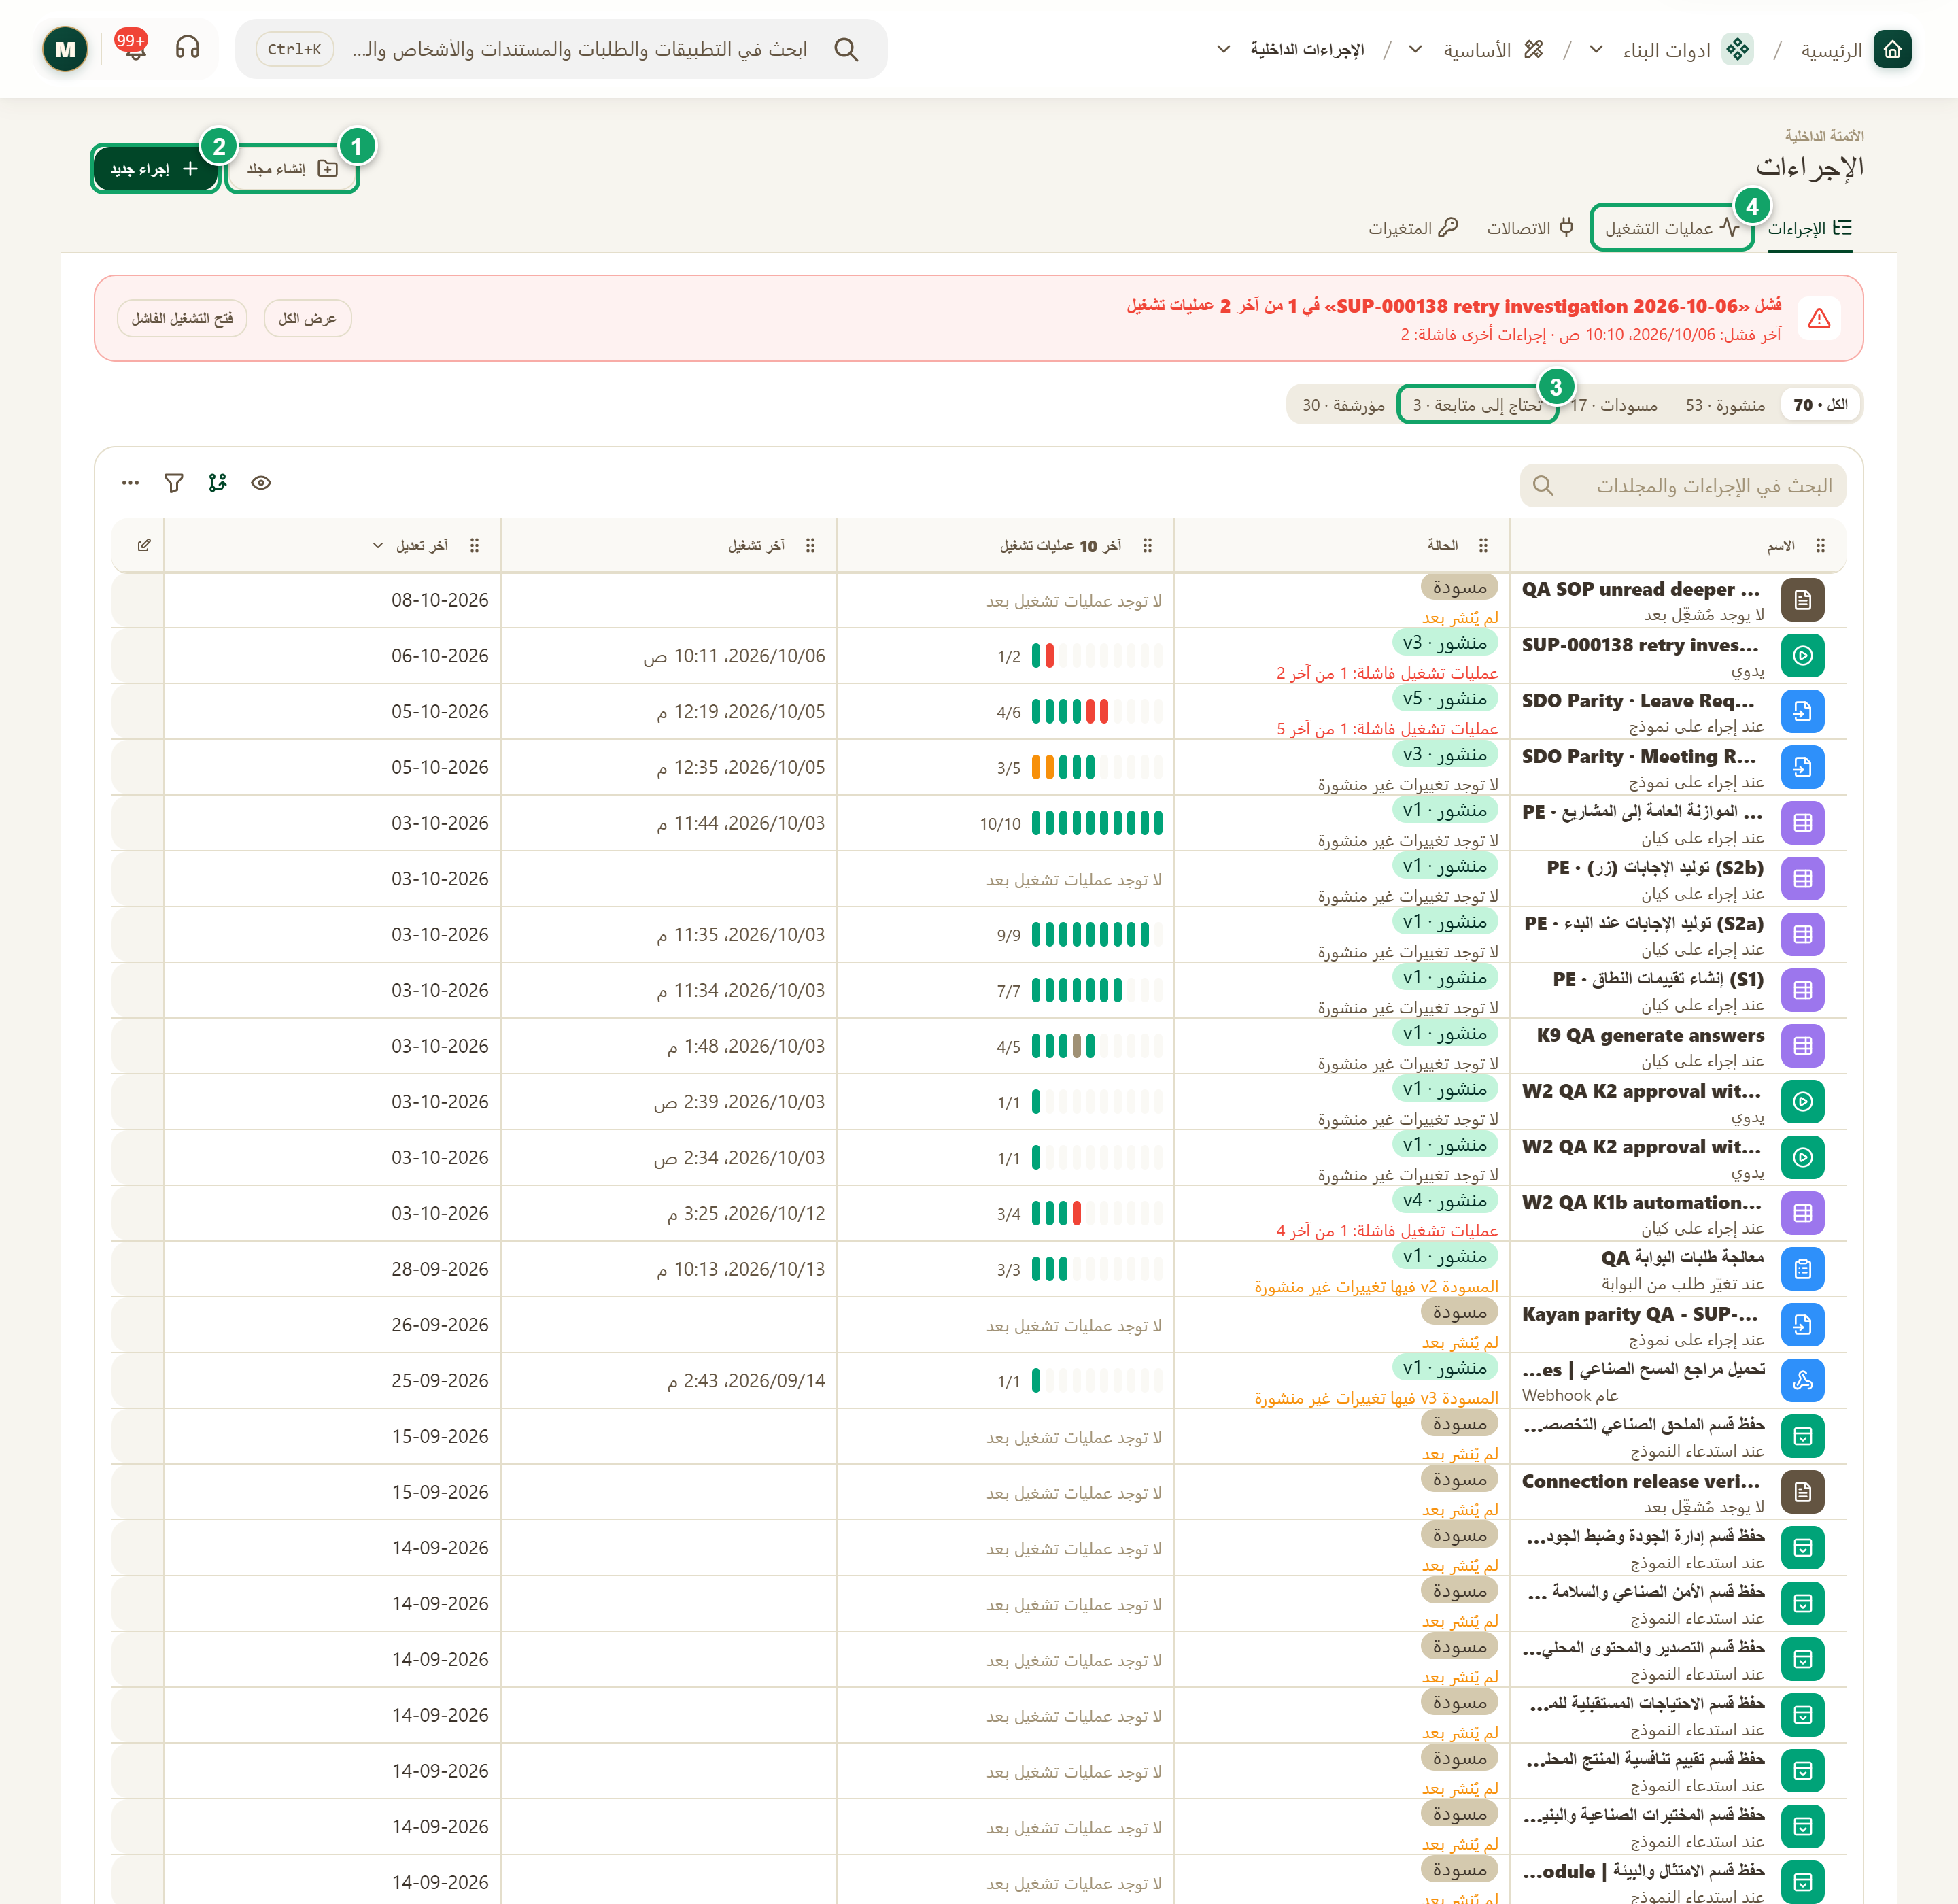
\includegraphics[width=0.95\linewidth,height=0.72\textheight,keepaspectratio]{figures/screens/ch06-internal-sops-ar.png}
\caption{صفحة «الإجراءات الداخلية»}
\label{fig:builder-internal-sops-screen}
\shotnote{تعرض الصورة أعلى قائمة الإجراءات في مؤسسة الاختبار، وفيها عشرات الإجراءات الاختبارية بحالاتها ونتائج آخر عمليات تشغيلها، ويسبقها تنبيه بإجراء فشل مؤخراً. وتبيّن الصورة أن الصفحة نفسها تنبهك إلى الإجراء المتعثر قبل أن تبحث عنه. ① «إنشاء مجلد»: ينظّم الإجراءات في مجلدات. ② «إجراء جديد»: يبدأ إجراءً ويطلب ما الذي يبدأه. ③ «تحتاج إلى متابعة»: يعرض الإجراءات المنشورة التي فشلت عمليات تشغيلها مؤخراً. ④ «عمليات التشغيل»: آخر عمليات التشغيل لكل الإجراءات.}
\end{figure}

\begin{table}[H]
\centering
\caption{ما الذي تجده في الصفحة؟}
\label{tab:builder-internal-sops-data}
\begin{tabularx}{\linewidth}{R{3.6cm} Y}
\rcHeaderRow
\thh{الجزء} & \thh{ما يقدمه}\\
التبويبات & «الإجراءات» وهو التبويب الافتراضي، و«عمليات التشغيل» لكل الإجراءات، و«الاتصالات»، و«المتغيرات».\\
التصفية & «الكل» و«منشورة» و«مسودات» و«تحتاج إلى متابعة» و«مؤرشفة»، مع عدد الإجراءات بجانب كل خيار. ويظهر «متوقفة مؤقتًا» عند وجود إجراء موقوف.\\
أعمدة القائمة & اسم الإجراء ومشغّله، و«الحالة» مثل «منشور · \en{v2}» أو «مسودة»، و«آخر 10 عمليات تشغيل» بنسبة الناجح منها، و«آخر تشغيل»، و«آخر تعديل».\\
تنبيه الفشل & يظهر أعلى القائمة عندما يفشل إجراء منشور في واحدة على الأقل من آخر خمس عمليات تشغيل، ومعه «فتح التشغيل الفاشل» و«عرض الكل».\\
المجلدات & «إنشاء مجلد» في رأس الصفحة. ومن قائمة المجلد تعيد تسميته، وتنشئ داخله إجراءً أو مجلداً فرعياً، وتنقله، وتحذفه.\\
قائمة الإجراء & «نقل إلى» مجلد آخر، و«إيقاف الإجراء مؤقتًا» أو «استئناف» للإجراء المنشور، وأمر الأرشفة الذي يظهر باسم «الأرشيف»، و«استعادة» للإجراء المؤرشف.\\
\end{tabularx}
\end{table}

\subsection{إنشاء إجراء جديد}

يفتح زر «إجراء جديد» لوحة جانبية تطلب أمرين فقط: الاسم، والإجابة عن «ما الذي يبدأه؟». وتعرض اللوحة أكثر المشغّلات استخداماً، وهي «عند إرسال نموذج» و«إنشاء سجل جديد» و«جدولة» و«عند انتهاء موافقة» و«Webhook عام» و«يدوي»، أما بقية المشغّلات فتجدها خلف «مزيد من المُشغِّلات». ويمكنك تغيير الاسم والمشغّل لاحقاً من المحرر.

\begin{rcwarn}[حذف مجلد فيه إجراءات]
إذا حذفت مجلداً يحتوي على إجراءات أو مجلدات فرعية، يطلب منك النظام أن تختار مصير المحتوى: إما نقله إلى جذر القائمة، وإما أرشفته مع حذف المجلد. أما المجلد الفارغ فيُحذف مباشرة.
\end{rcwarn}

\begin{figure}[H]
\centering
\begin{tikzpicture}[node distance=0.5cm]
\node[stepBox] (a) {\RL{إجراء جديد}};
\node[stepBox,below=of a] (b) {\RL{كتابة الاسم}};
\node[stepBox,below=of b] (c) {\RL{اختيار ما الذي يبدأه}};
\node[stepBox,below=of c] (d) {\RL{إنشاء وفتح}};
\node[stepBox,below=of d] (e) {\RL{المحرر: بناء الخطوات}};
\draw[flowsTo] (a) -- (b);
\draw[flowsTo] (b) -- (c);
\draw[flowsTo] (c) -- (d);
\draw[flowsTo] (d) -- (e);
\end{tikzpicture}
\rclegend
\caption{إنشاء إجراء من الصفحة الرئيسية}
\label{fig:builder-internal-sops-flow}
\shotnote{يبيّن المخطط أن الإجراء لا يُنشأ دون مشغّل، لأن الزر «إنشاء وفتح» يبقى معطلاً حتى تختار ما الذي يبدأه. وبعد الإنشاء تنتقل مباشرة إلى المحرر، فيكون الإجراء مسودة لا تعمل حتى تنشرها.}
\end{figure}

\subsection{خطوات العمل والتحقق}
\begin{enumerate}
\item افتح «الإجراءات الداخلية»، وإذا أردت ترتيب الإجراءات فاضغط «إنشاء مجلد» واكتب «اسم المجلد».
\item اضغط «إجراء جديد»، أو اختر من قائمة المجلد أمر إنشاء الإجراء داخله.
\item اكتب الاسم، واختر مشغّلاً من الخيارات الشائعة أو من «مزيد من المُشغِّلات»، ثم اضغط «إنشاء وفتح».
\item عُد إلى القائمة لاحقاً، واختر «تحتاج إلى متابعة» لترى الإجراءات المنشورة التي فشلت عمليات تشغيلها مؤخراً.
\end{enumerate}

\textbf{تحقق ومعالجة المشكلة:} يجب أن يفتح المحرر على الإجراء الجديد، وأن يظهر في القائمة بحالة «مسودة» مع ملاحظة «لم يُنشر بعد». فإذا لم تجد إجراءً تعرفه، فاختر «الكل» وامسح البحث، ثم جرّب «مؤرشفة»؛ فالإجراء المؤرشف لا يظهر في «الكل» حتى تستعيده بأمر «استعادة».

\clearpage
\section{محرر الإجراء وأوضاعه}
\label{sec:builder-feature-isop-editor}

المحرر هو المكان الذي ترسم فيه الإجراء خطوة بعد خطوة. ويتكون من رأس يعرض حالة الإجراء، وقائمة «الخطوات» بجانب اللوحة، ولوحة ترى عليها الخطوات والمسارات بينها. ويعمل المحرر في ثلاثة أوضاع: «بناء» لتعديل الخطوات، و«اختبار» لتجربة المسودة، و«عمليات التشغيل» لرؤية ما حدث في كل تشغيل على اللوحة نفسها. وتُحفظ تعديلاتك تلقائياً في مسودة.

\textbf{المسار ومن يستخدمه:} «الإجراءات الداخلية» ← اضغط اسم الإجراء. يستخدمه من يبني الإجراء أو يصلحه.

\begin{rcnote}[مثال: شركة الأفق]
يفتح المسؤول إجراء «اعتماد طلب الزيارة» فيرى في قائمة «الخطوات» أن خطوة «طلب موافقة» تحمل الشارة «يحتاج إلى تهيئة». فيضغطها، ويكمل إعدادها، ثم يكتب على اللوحة ملاحظة (③) تشرح لزملائه سبب طلب موافقة سارة.
\end{rcnote}

\begin{figure}[H]
\centering
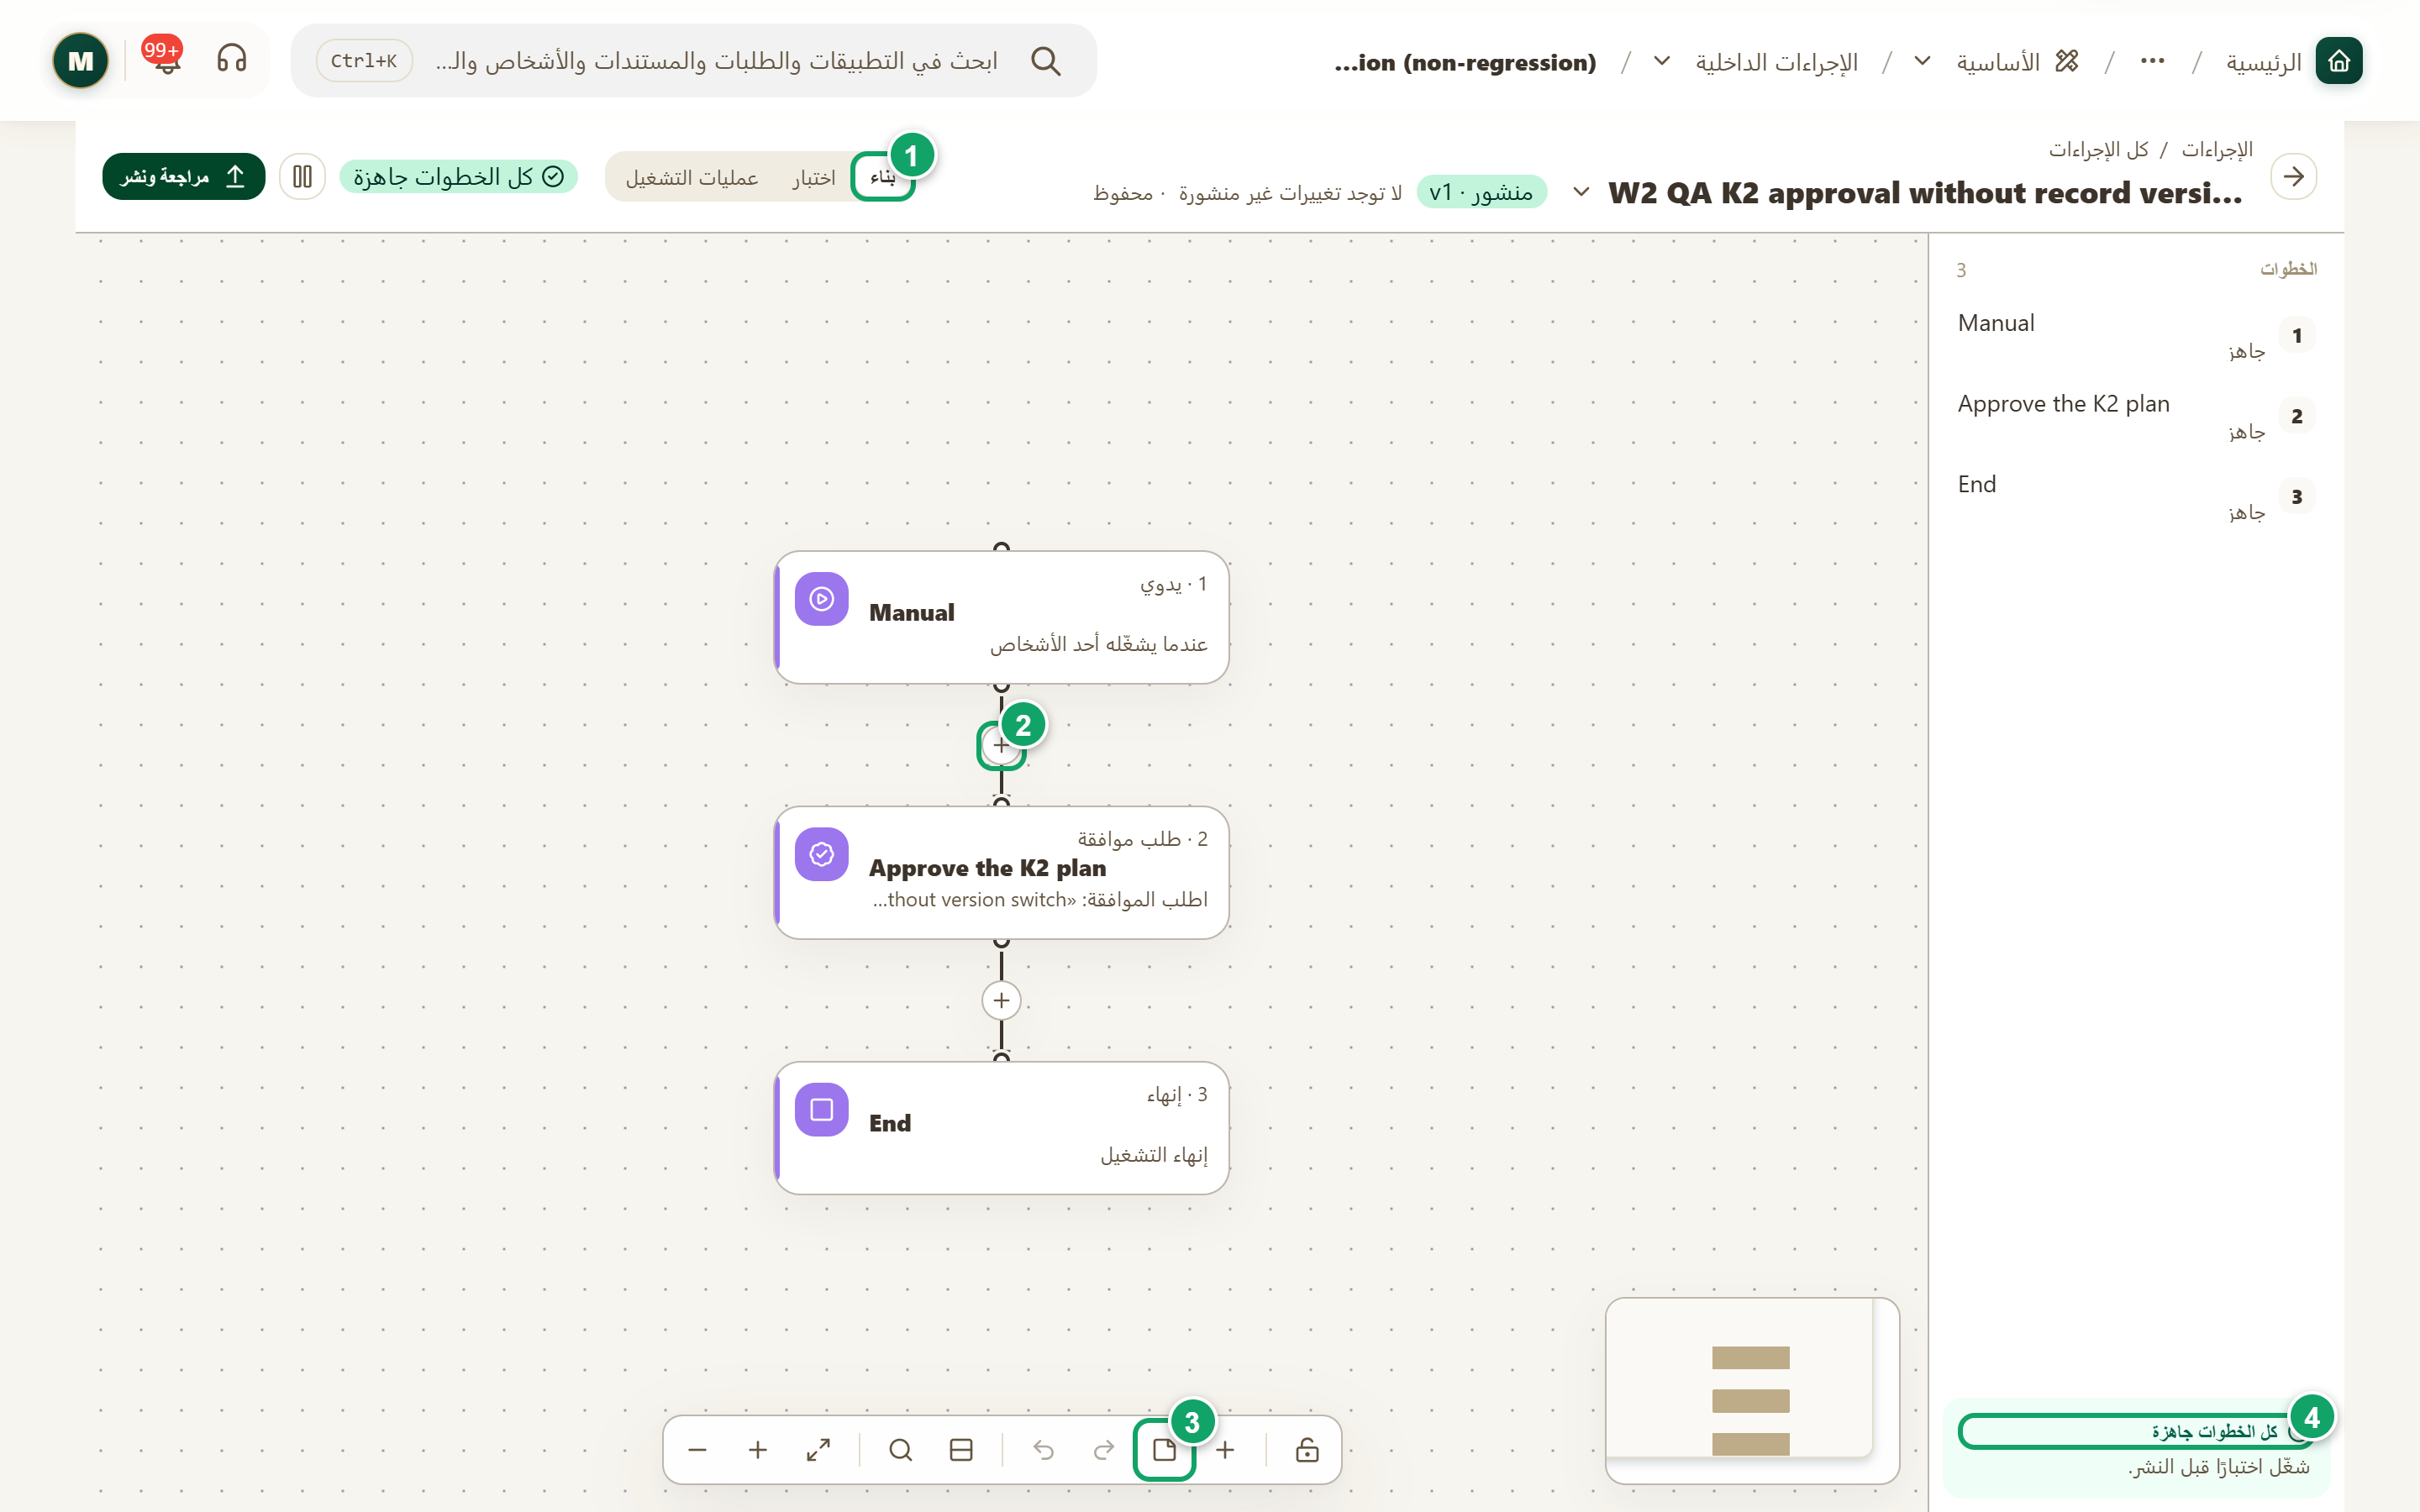
\includegraphics[width=0.95\linewidth,height=0.72\textheight,keepaspectratio]{figures/screens/ch06-isop-editor-ar.png}
\caption{محرر إجراء قائم في وضع «بناء»}
\label{fig:builder-isop-editor-screen}
\shotnote{تعرض الصورة إجراءً اختبارياً منشوراً في مؤسسة الاختبار، مفتوحاً في وضع «بناء» وكل خطواته جاهزة. ويجمع المحرر في شاشة واحدة قائمة الخطوات واللوحة وأدواتها، فتعرف حالة الإجراء قبل أن تعدّل فيه. ① «بناء»: الوضع الذي تعدّل فيه الخطوات. ② زر الإضافة «+» على الخط بين خطوتين: يفتح قائمة الخطوات. ③ «إضافة ملاحظة»: يضع على اللوحة ملاحظة لزملائك. ④ «كل الخطوات جاهزة»: ملخص قائمة الخطوات حين لا تحتاج أي خطوة إلى تهيئة.}
\end{figure}

\begin{table}[H]
\centering
\caption{أجزاء المحرر}
\label{tab:builder-isop-editor-parts}
\begin{tabularx}{\linewidth}{R{3.6cm} Y}
\rcHeaderRow
\thh{الجزء} & \thh{ما يقدمه}\\
رأس المحرر & «العودة إلى الإجراءات»، واسم الإجراء الذي يفتح تفاصيله وسجل إصداراته، وشارة الإصدار مثل «منشور · \en{v2}» أو «لم يُنشر بعد»، وحالة الحفظ مثل «محفوظ».\\
الأوضاع & «بناء» و«اختبار» و«عمليات التشغيل». ويظهر بجانبها اتصال الخادم: «متصل» أو «الخادم غير متصل».\\
شارة الجاهزية & «N للإصلاح» إذا بقيت خطوات ناقصة، أو «كل الخطوات جاهزة». والضغط عليها يفتح المراجعة.\\
الخطوات & قائمة مرقّمة بترتيب الخطوات، وتحت كل خطوة حالتها، مثل «جاهز» أو «يحتاج إلى تهيئة». وفوقها ملخص «خطوات تحتاج إلى تهيئة: N» أو «كل الخطوات جاهزة».\\
اللوحة & تضيف خطوة بزر الإضافة على الخط بين خطوتين، وتفتح قائمة الخطوة بالنقر بالزر الأيمن لنسخها أو لصقها أو اختبارها أو حذفها.\\
أدوات اللوحة & «إضافة مشغّل»، و«إضافة ملاحظة»، والتخطيط الأفقي أو العمودي، والتكبير والتصغير، و«ملاءمة سير العمل للعرض»، والبحث في الخطوات، والخريطة المصغرة، و«تراجع» و«إعادة».\\
\end{tabularx}
\end{table}

\subsection{إضافة خطوة}

عندما تضغط زر الإضافة تظهر قائمة الخطوات مقسّمة إلى أربع فئات: «تدفق التحكم» و«Kayan» و«خدمات المتعاملين» و«التكاملات». وتنقسم فئة «Kayan» إلى أقسام، مثل «السجلات» و«النماذج» و«المهام والمشاريع» و«الموافقات والطلبات» و«الإشعارات والمحادثات» و«المستندات». ويمكنك أن تبحث مباشرة في «ابحث عن التطبيقات والإجراءات» بدلاً من التنقل بين الفئات.

\begin{figure}[H]
\centering
\begin{tikzpicture}[node distance=0.5cm]
\node[stepBox] (a) {\RL{فتح الإجراء في وضع بناء}};
\node[stepBox,below=of a] (b) {\RL{إضافة خطوة من القائمة}};
\node[stepBox,below=of b] (c) {\RL{إعداد الخطوة}};
\node[stepBox,below=of c] (d) {\RL{مراجعة قائمة الخطوات}};
\node[stepBox,below=of d] (e) {\RL{الانتقال إلى اختبار}};
\draw[flowsTo] (a) -- (b);
\draw[flowsTo] (b) -- (c);
\draw[flowsTo] (c) -- (d);
\draw[flowsTo] (d) -- (e);
\end{tikzpicture}
\rclegend
\caption{جلسة بناء في المحرر}
\label{fig:builder-isop-editor-flow}
\shotnote{يوضح المخطط أن إضافة الخطوة وإعدادها عمل واحد يتكرر حتى تكتمل كل الخطوات. وتأتي مراجعة قائمة «الخطوات» قبل الاختبار، لأنها تكشف الخطوات الناقصة التي قد يتوقف عندها الاختبار.}
\end{figure}

\subsection{خطوات العمل والتحقق}
\begin{enumerate}
\item افتح الإجراء من «الإجراءات الداخلية»، وتأكد أن الوضع «بناء».
\item اضغط زر الإضافة على الخط بعد المشغّل، واختر الخطوة من فئتها أو بالبحث.
\item اضغط الخطوة على اللوحة لتفتح إعدادها، وأكمل حقولها المطلوبة.
\item أضف ملاحظة من «إضافة ملاحظة» إذا أردت أن تشرح جزءاً من المسار لزملائك.
\item راجع ملخص قائمة «الخطوات» حتى يظهر «كل الخطوات جاهزة».
\end{enumerate}

\textbf{تحقق ومعالجة المشكلة:} يجب أن تتغير حالة الحفظ إلى «محفوظ» بعد كل تعديل، وأن تظهر الخطوة الجديدة في قائمة «الخطوات» برقمها. فإذا حذفت خطوة بالخطأ، فاضغط «تراجع» أو \en{Ctrl+Z}. وإذا ظهر «الخادم غير متصل»، فتستطيع التعديل، لكنك لن تستطيع الاختبار أو النشر حتى يعود الاتصال.

\clearpage
\section{المشغّلات: ما الذي يبدأ الإجراء؟}
\label{sec:builder-feature-isop-triggers}

المشغّل هو الحدث الذي يبدأ عملية تشغيل جديدة للإجراء، وهو دائماً الخطوة الأولى في المسار. فقد يكون حدثاً في النظام مثل إنشاء سجل أو إرسال نموذج، أو موعداً متكرراً، أو ضغطة من أحد الأعضاء. ولا يعمل المشغّل إلا بعد نشر الإجراء، ويمكن أن يحتوي الإجراء على أكثر من مشغّل.

\textbf{المسار ومن يستخدمه:} لوحة «إجراء جديد» ← «ما الذي يبدأه؟» ← «مزيد من المُشغِّلات»، أو في المحرر «إضافة مشغّل»، أو «تغيير المشغّل» من إعداد خطوة المشغّل. يستخدمها من يبني الإجراء.

\begin{rcnote}[مثال: شركة الأفق]
يختار المسؤول «إنشاء سجل جديد» (④)، ثم يحدد في «الجدول» نوع السجلات «طلبات الزيارة». فكلما أضاف عمر حداد طلباً جديداً مثل \en{HZN-VR-0001}، بدأت عملية تشغيل جديدة للإجراء.
\end{rcnote}

\begin{figure}[H]
\centering
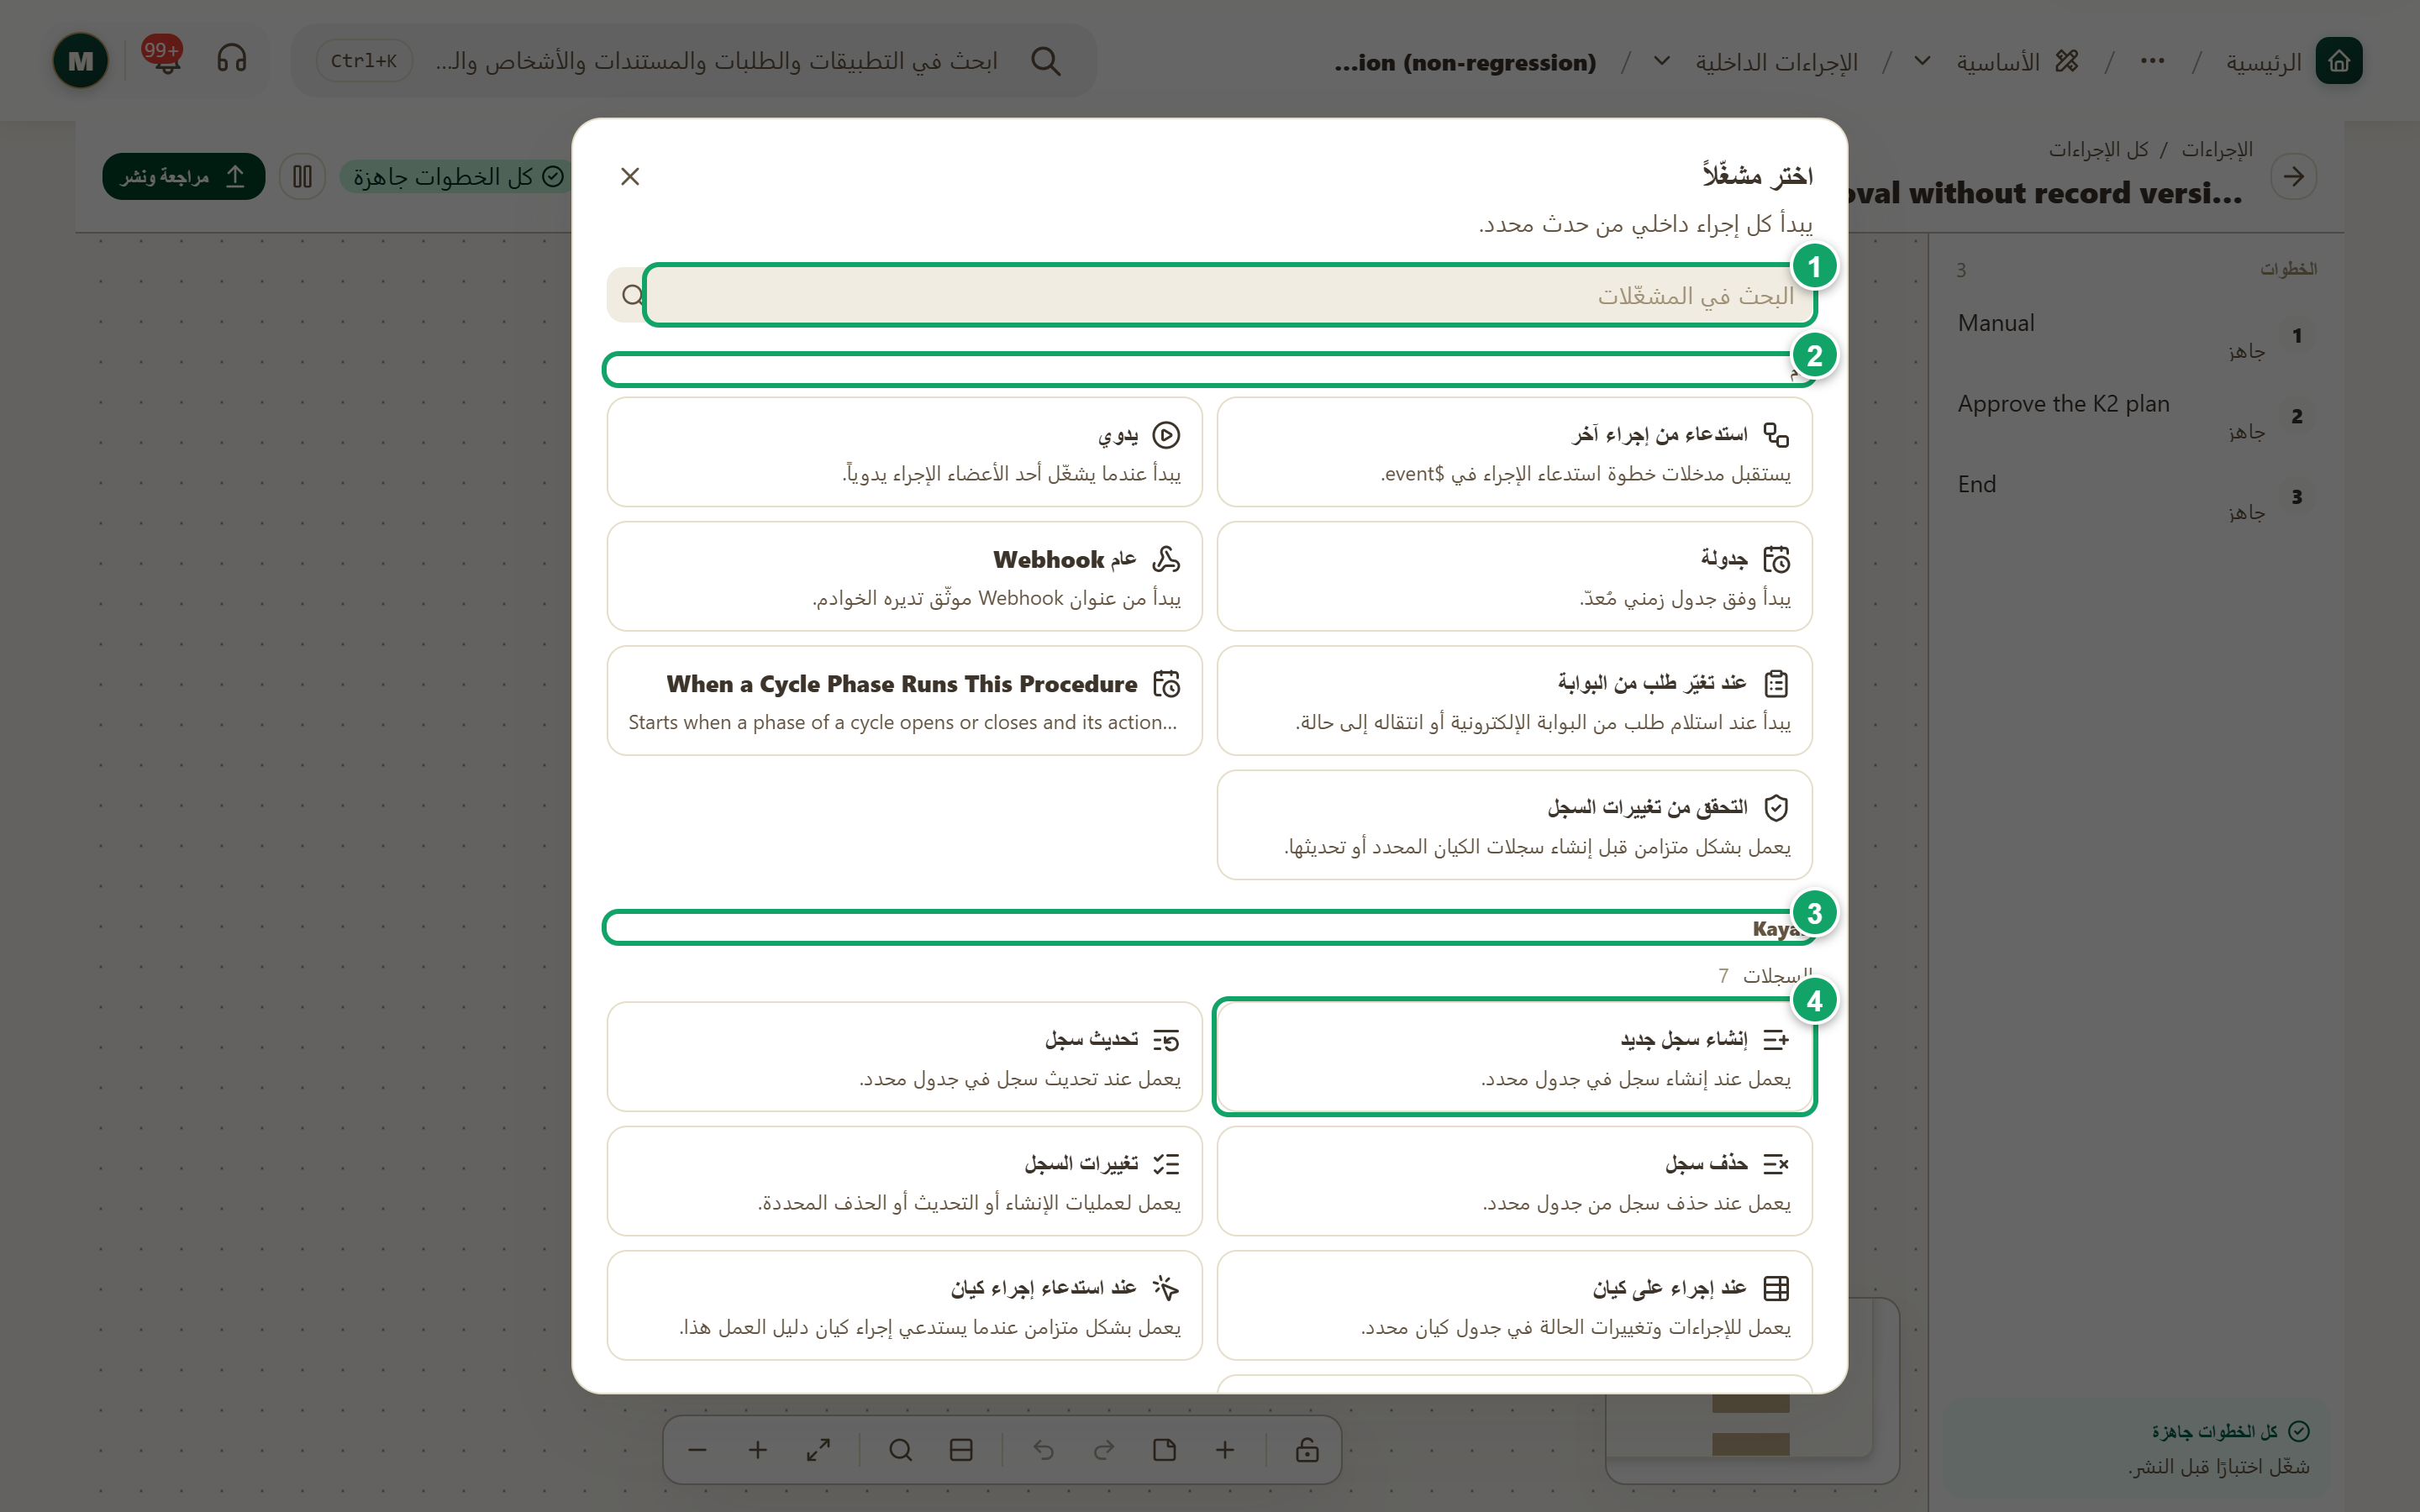
\includegraphics[width=0.95\linewidth,height=0.72\textheight,keepaspectratio]{figures/screens/ch06-isop-triggers-ar.png}
\caption{نافذة «اختر مشغّلاً»}
\label{fig:builder-isop-triggers-screen}
\shotnote{تعرض الصورة النافذة التي تفتح من «إضافة مشغّل»، وفيها المشغّلات مجمّعة تحت «عام» ثم «Kayan» مقسّمة إلى أقسام، وتليها مشغّلات التكاملات عند التمرير. وتفيدك المجموعات في الوصول إلى الحدث المناسب دون حفظ أسماء المشغّلات كلها. ① «البحث في المشغّلات»: تكتب فيه اسم الحدث مباشرة. ② «عام»: المشغّلات اليدوية والمجدولة والمستدعاة. ③ «Kayan»: أحداث النظام مقسّمة حسب القسم. ④ «إنشاء سجل جديد»: مثال على مشغّل يعمل عند إنشاء سجل في جدول تختاره.}
\end{figure}

\begin{table}[H]
\centering
\caption{مجموعات المشغّلات في نافذة «اختر مشغّلاً»}
\label{tab:builder-isop-triggers-groups}
\begin{tabularx}{\linewidth}{R{3.6cm} Y}
\rcHeaderRow
\thh{المجموعة} & \thh{أمثلة ومتى تستخدمها}\\
عام & «يدوي» عندما يشغّل أحد الأعضاء الإجراء بنفسه، و«جدولة» لموعد يومي أو أسبوعي أو بتعبير \en{Cron}، و«Webhook عام» عندما يستدعي نظام آخر رابط الإجراء، و«استدعاء من إجراء آخر» للإجراء الذي تستدعيه خطوة من إجراء آخر. ويوجد كذلك مشغّل يبدأ الإجراء عندما تفتح مرحلة من «الدورات» أو تُغلق وتسمّي الإجراء في إجراءاتها.\\
\en{Kayan} & أحداث النظام مقسّمة حسب القسم، كالسجلات والنماذج والمهام والموافقات والملفات والدعم والبريد وواتساب.\\
التكاملات & أحداث من خدمات خارجية، وتحتاج عادةً إلى اتصال بحساب تلك الخدمة.\\
\end{tabularx}
\end{table}

\begin{table}[H]
\centering
\caption{مشغّلات السجلات والنماذج والمهام والموافقات}
\label{tab:builder-isop-triggers-kayan}
\begin{tabularx}{\linewidth}{R{3.6cm} Y}
\rcHeaderRow
\thh{المشغّل} & \thh{متى يبدأ الإجراء}\\
إنشاء سجل جديد، تحديث سجل، حذف سجل & عند إنشاء سجل أو تحديثه أو حذفه في «الجدول» الذي تختاره. أما «تغييرات السجل» فيجمع العمليات التي تحددها منها.\\
عند إجراء على كيان & عند تنفيذ إجراء أو تغيير حالة في نوع سجلات محدد، مثل انتقال الطلب إلى حالة الاعتماد.\\
عند إرسال نموذج & عند إرسال أي جلسة نموذج في النظام.\\
عند إجراء على نموذج & عندما ينفّذ نموذج محدد أحد الإجراءات التي تختارها.\\
عند إجراء على مهمة & عند تنفيذ إجراءات مهمة أو تغيّر حالتها. ويوجد مشغّل مستقل عند إضافة تعليق إلى مهمة.\\
عند استجابة موافقة، عند انتهاء موافقة & الأول مع كل رد على طلب موافقة، والثاني عندما يكتمل الطلب أو يُلغى أو تنتهي مهلته.\\
\end{tabularx}
\end{table}

\begin{rcwarn}[تغيير المشغّل يحذف إعداده]
إذا ضغطت «تغيير المشغّل» بعد إعداده، تظهر رسالة «هل تريد تغيير المشغّل؟» مع قائمة الحقول التي ستُحذف. فاضغط «متابعة» فقط إذا كنت ستعيد إعداد المشغّل الجديد.
\end{rcwarn}

\begin{figure}[H]
\centering
\begin{tikzpicture}[node distance=0.5cm]
\node[stepBox] (a) {\RL{اختر مشغّلاً}};
\node[stepBox,below=of a] (b) {\RL{البحث أو اختيار المجموعة}};
\node[stepBox,below=of b] (c) {\RL{إعداد حقول المشغّل}};
\node[stepBox,below=of c] (d) {\RL{إضافة خطوة بعده}};
\node[stepBox,below=of d] (e) {\RL{النشر ليبدأ العمل}};
\draw[flowsTo] (a) -- (b);
\draw[flowsTo] (b) -- (c);
\draw[flowsTo] (c) -- (d);
\draw[flowsTo] (d) -- (e);
\end{tikzpicture}
\rclegend
\caption{إعداد المشغّل}
\label{fig:builder-isop-triggers-flow}
\shotnote{يربط المخطط بين المشغّل والنشر، لأن المشغّل في المسودة لا يبدأ أي عملية تشغيل. ويذكّرك بإضافة خطوة بعده، فالمراجعة ترفض النشر برسالة «أضف خطوة بعد هذا المُشغِّل» إذا بقي وحده.}
\end{figure}

\subsection{خطوات العمل والتحقق}
\begin{enumerate}
\item في المحرر، اضغط «إضافة مشغّل»، أو افتح المشغّل الحالي واضغط «تغيير المشغّل».
\item ابحث في «البحث في المشغّلات» باسم الحدث، أو تصفح «عام» و\en{Kayan} و«التكاملات».
\item اختر المشغّل، ثم أكمل حقوله، مثل «الجدول» لمشغّلات السجلات أو التكرار والوقت والمنطقة الزمنية لـ«جدولة».
\item أضف خطوة بعد المشغّل، ثم انشر الإجراء.
\end{enumerate}

\textbf{تحقق ومعالجة المشكلة:} بعد النشر يجب أن تظهر عملية تشغيل جديدة في «عمليات التشغيل» كلما وقع الحدث. فإذا لم تظهر، فتأكد أن الإجراء ليس «متوقفاً مؤقتاً»، وأنك اخترت الجدول أو النموذج الصحيح في المشغّل. ولمشغّل «Webhook عام» يظهر «رابط الويب هوك المنشور» بعد النشر فقط.

\clearpage
\section{خطوات التحكم في المسار}
\label{sec:builder-feature-isop-control-flow}

خطوات التحكم لا تنفّذ عملاً في النظام، بل تحدد طريق الإجراء: هل يتفرّع؟ هل يكرر خطوة لكل عنصر في قائمة؟ هل ينتظر مدة أو حدثاً؟ متى ينتهي؟ وتجدها كلها في فئة «تدفق التحكم» عند إضافة خطوة. وبفضلها يتبع الإجراء القاعدة التي تعمل بها المؤسسة فعلاً، لا مساراً واحداً ثابتاً.

\textbf{المسار ومن يستخدمه:} المحرر ← زر الإضافة ← «تدفق التحكم». يستخدمها من يبني الإجراء.

\begin{rcnote}[مثال: شركة الأفق]
يضيف المسؤول بعد «طلب موافقة» خطوة «تفرّع شرطي» (②) لها مساران: الأول يتابع إلى إنشاء مهمة عمر إذا كانت النتيجة موافقة، والثاني ينتهي بخطوة «إنهاء» إذا طلبت سارة تغييرات.
\end{rcnote}

\begin{figure}[H]
\centering
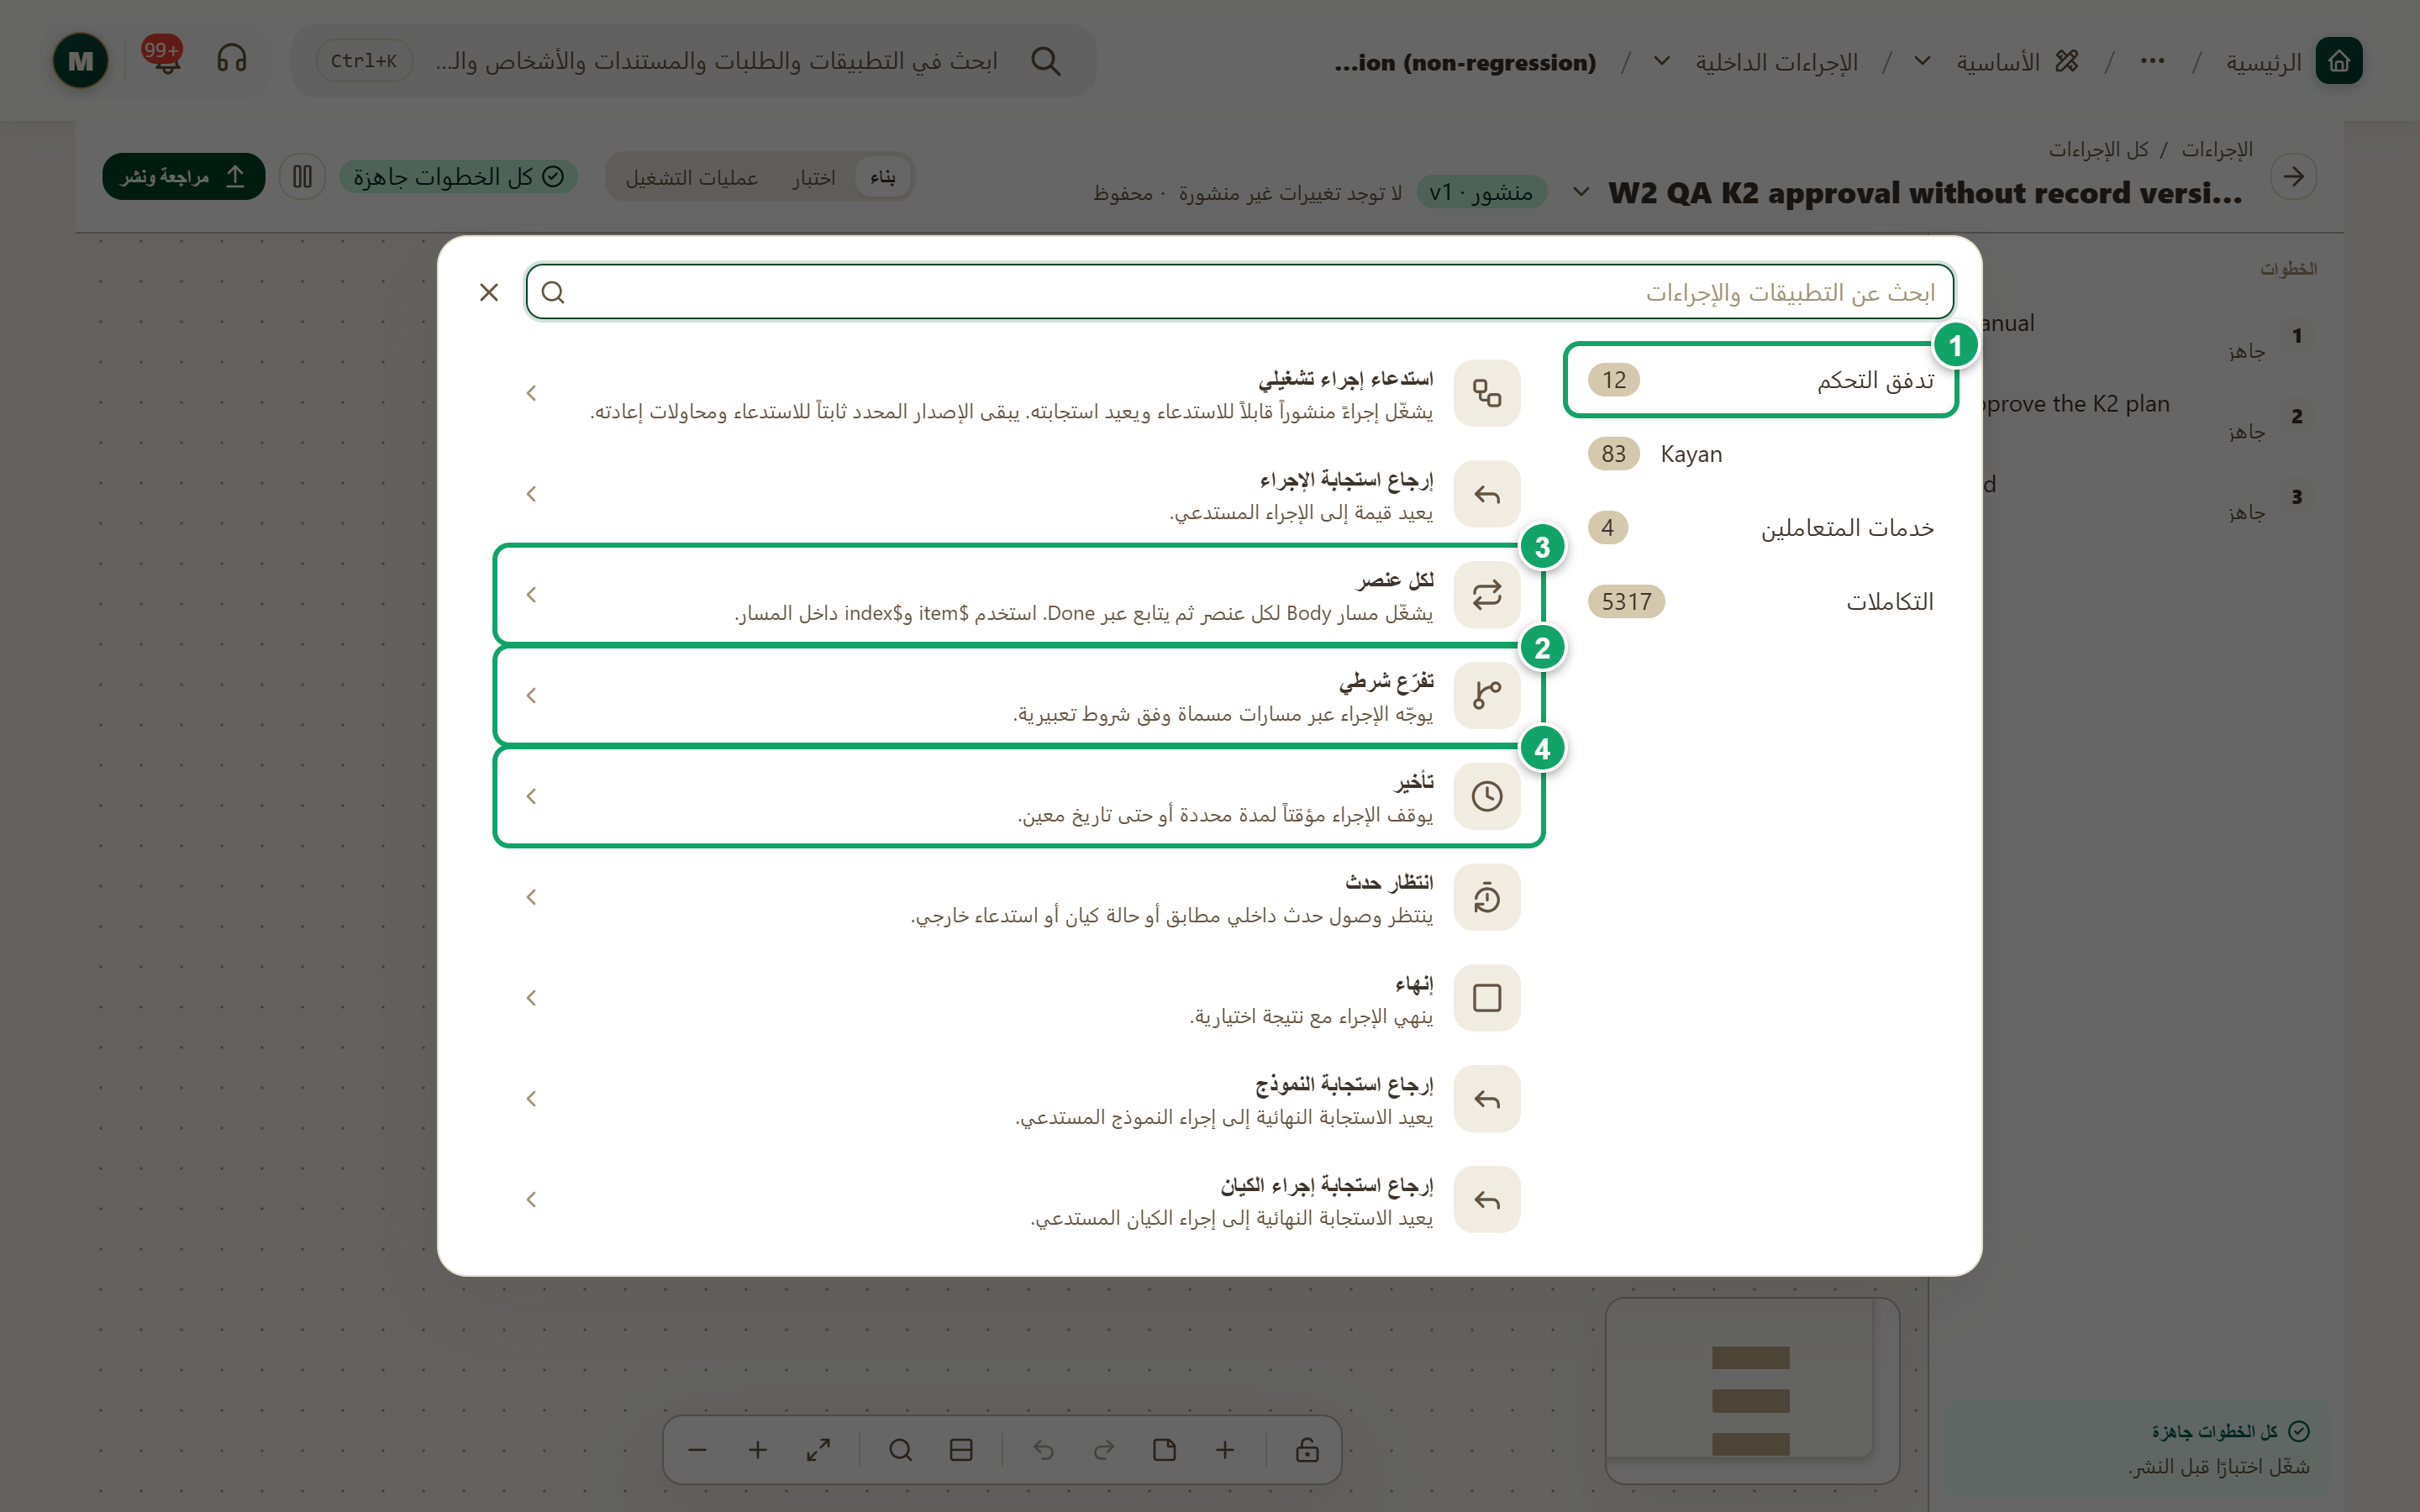
\includegraphics[width=0.95\linewidth,height=0.72\textheight,keepaspectratio]{figures/screens/ch06-isop-control-flow-ar.png}
\caption{فئة «تدفق التحكم» في قائمة الخطوات}
\label{fig:builder-isop-control-flow-screen}
\shotnote{تعرض الصورة قائمة الخطوات بعد الضغط على زر الإضافة، وقد فُتحت على فئة «تدفق التحكم» بخطواتها الاثنتي عشرة ووصف مختصر لكل منها. ويساعدك الوصف على اختيار الخطوة التي تحدد طريق الإجراء قبل أن تضيفها. ① «تدفق التحكم»: الفئة التي تجمع خطوات التحكم. ② «تفرّع شرطي»: يوجّه الإجراء إلى مسارات مسمّاة. ③ «لكل عنصر»: يكرر خطوات لكل عنصر في قائمة. ④ «تأخير»: يوقف الإجراء مدة محددة أو حتى تاريخ.}
\end{figure}

\begin{table}[H]
\centering
\caption{خطوات «تدفق التحكم»}
\label{tab:builder-isop-control-flow-steps}
\begin{tabularx}{\linewidth}{R{3.6cm} Y}
\rcHeaderRow
\thh{الخطوة} & \thh{ما تفعله}\\
تفرّع شرطي & يوجّه الإجراء إلى مسارات مسمّاة، لكل مسار تسمية وشرط. وتبدأ بمسارين ومسار بديل عند عدم المطابقة، وتختار في «المسارات المطابقة» بين «أول مسار مطابق» و«كل المسارات المطابقة».\\
لكل عنصر & يكرر خطوات جسم الحلقة لكل عنصر في «العناصر»، ثم يتابع بعد انتهائها. وداخل الحلقة تستطيع استخدام العنصر الحالي وموضعه.\\
تأخير & يوقف الإجراء «لمدة محددة» مثل يوم واحد، أو «حتى تاريخ معين».\\
انتظار حدث & ينتظر حتى يصل حدث داخلي أو حالة سجل أو استدعاء خارجي يطابق ما تحدده، مع مهلة اختيارية.\\
إنهاء & ينهي التشغيل مع نتيجة اختيارية، ولا يمكن أن تتبعه أي خطوة.\\
استدعاء إجراء تشغيلي & يشغّل إجراءً منشوراً مشغّله «استدعاء من إجراء آخر»، وينتظر استجابته. ويثبت الإصدار المختار للاستدعاء نفسه حتى عند إعادة المحاولة.\\
إرجاع استجابة الإجراء & يعيد قيمة إلى الإجراء الذي استدعى هذا الإجراء.\\
تشغيل \en{JavaScript} & يشغّل شيفرة قصيرة في بيئة معزولة دون شبكة، ويعيد قيمة تستخدمها الخطوات التالية.\\
\end{tabularx}
\end{table}

\begin{rcwarn}[القرار وحده يتفرّع]
لا يمكن أن تخرج من خطوة عادية إلا وصلة واحدة. فإذا أردت مسارين، فأضف «تفرّع شرطي»، وإلا ظهرت مشكلة «القرار وحده يمكنه التفرّع إلى عدة مسارات». وكذلك يجب أن يحمل كل مسار في القرار اسماً.
\end{rcwarn}

\begin{figure}[H]
\centering
\begin{tikzpicture}[node distance=0.5cm]
\node[stepBox] (a) {\RL{خطوة سابقة تعيد نتيجة}};
\node[stepBox,below=of a] (b) {\RL{تفرّع شرطي}};
\node[stepBox,below=of b] (c) {\RL{المسار المطابق}};
\node[stepBox,below=of c] (d) {\RL{تأخير أو انتظار حدث}};
\node[stepBox,below=of d] (e) {\RL{إنهاء}};
\draw[flowsTo] (a) -- (b);
\draw[flowsTo] (b) -- (c);
\draw[flowsTo] (c) -- (d);
\draw[flowsTo] (d) -- (e);
\end{tikzpicture}
\rclegend
\caption{كيف تقود خطوات التحكم المسار}
\label{fig:builder-isop-control-flow-flow}
\shotnote{يبيّن المخطط أن القرار يعتمد على نتيجة خطوة سبقته، فلا معنى لشرط لا يجد بيانات يقرؤها. أما التأخير والانتظار فيجعلان التشغيل في حالة «بانتظار استجابة» حتى يحين الموعد أو يصل الحدث، ثم يتابع المسار حتى «إنهاء».}
\end{figure}

\subsection{خطوات العمل والتحقق}
\begin{enumerate}
\item أضف «تفرّع شرطي» بعد الخطوة التي تريد أن تقرر بناءً على نتيجتها.
\item في إعداد القرار، اكتب تسمية كل مسار، واضغط «حدّد الشرط» لتكتب الشرط أو تختار «دائمًا» أو «أبدًا».
\item اضغط «إضافة مسار» إذا احتجت مساراً آخر، واختر في «المسارات المطابقة» طريقة الاختيار.
\item أضف إلى نهاية كل مسار الخطوة التالية أو خطوة «إنهاء».
\end{enumerate}

\textbf{تحقق ومعالجة المشكلة:} يجب أن ترى على اللوحة خطاً لكل مسار يحمل تسميته، وأن يختفي تنبيه «شروط القرار لا تطابق مساراته». وإذا سلك الاختبار المسار الخطأ، فافتح نتيجة الخطوة السابقة في الاختبار وتحقق من القيمة التي يقرؤها الشرط.

\clearpage
\section{خطوات السجلات والنماذج}
\label{sec:builder-feature-isop-records}

تتعامل هذه الخطوات مع البيانات المحفوظة في أنواع السجلات ومع النماذج. فتستطيع بها أن تبحث عن سجلات، أو تُنشئ سجلاً، أو تحدّث حقول سجل موجود، أو تطلب من الأعضاء تعبئة نموذج. وتجدها في فئة \en{Kayan} ضمن قسمي «السجلات» و«النماذج».

\textbf{المسار ومن يستخدمه:} المحرر ← زر الإضافة ← \en{Kayan} ← «السجلات» أو «النماذج». يستخدمها من يبني الإجراء، ويحتاج إلى صلاحية على أنواع السجلات التي تتعامل معها الخطوة.

\begin{rcnote}[مثال: شركة الأفق]
يضيف المسؤول خطوة «تحديث سجل كيان» (⑤) بعد موافقة سارة الخطيب، فيختار نوع السجلات «طلبات الزيارة» ويضع في «السجل» السجل الذي بدأ التشغيل، ثم يعيّن حالة الطلب إلى معتمد.
\end{rcnote}

\begin{figure}[H]
\centering
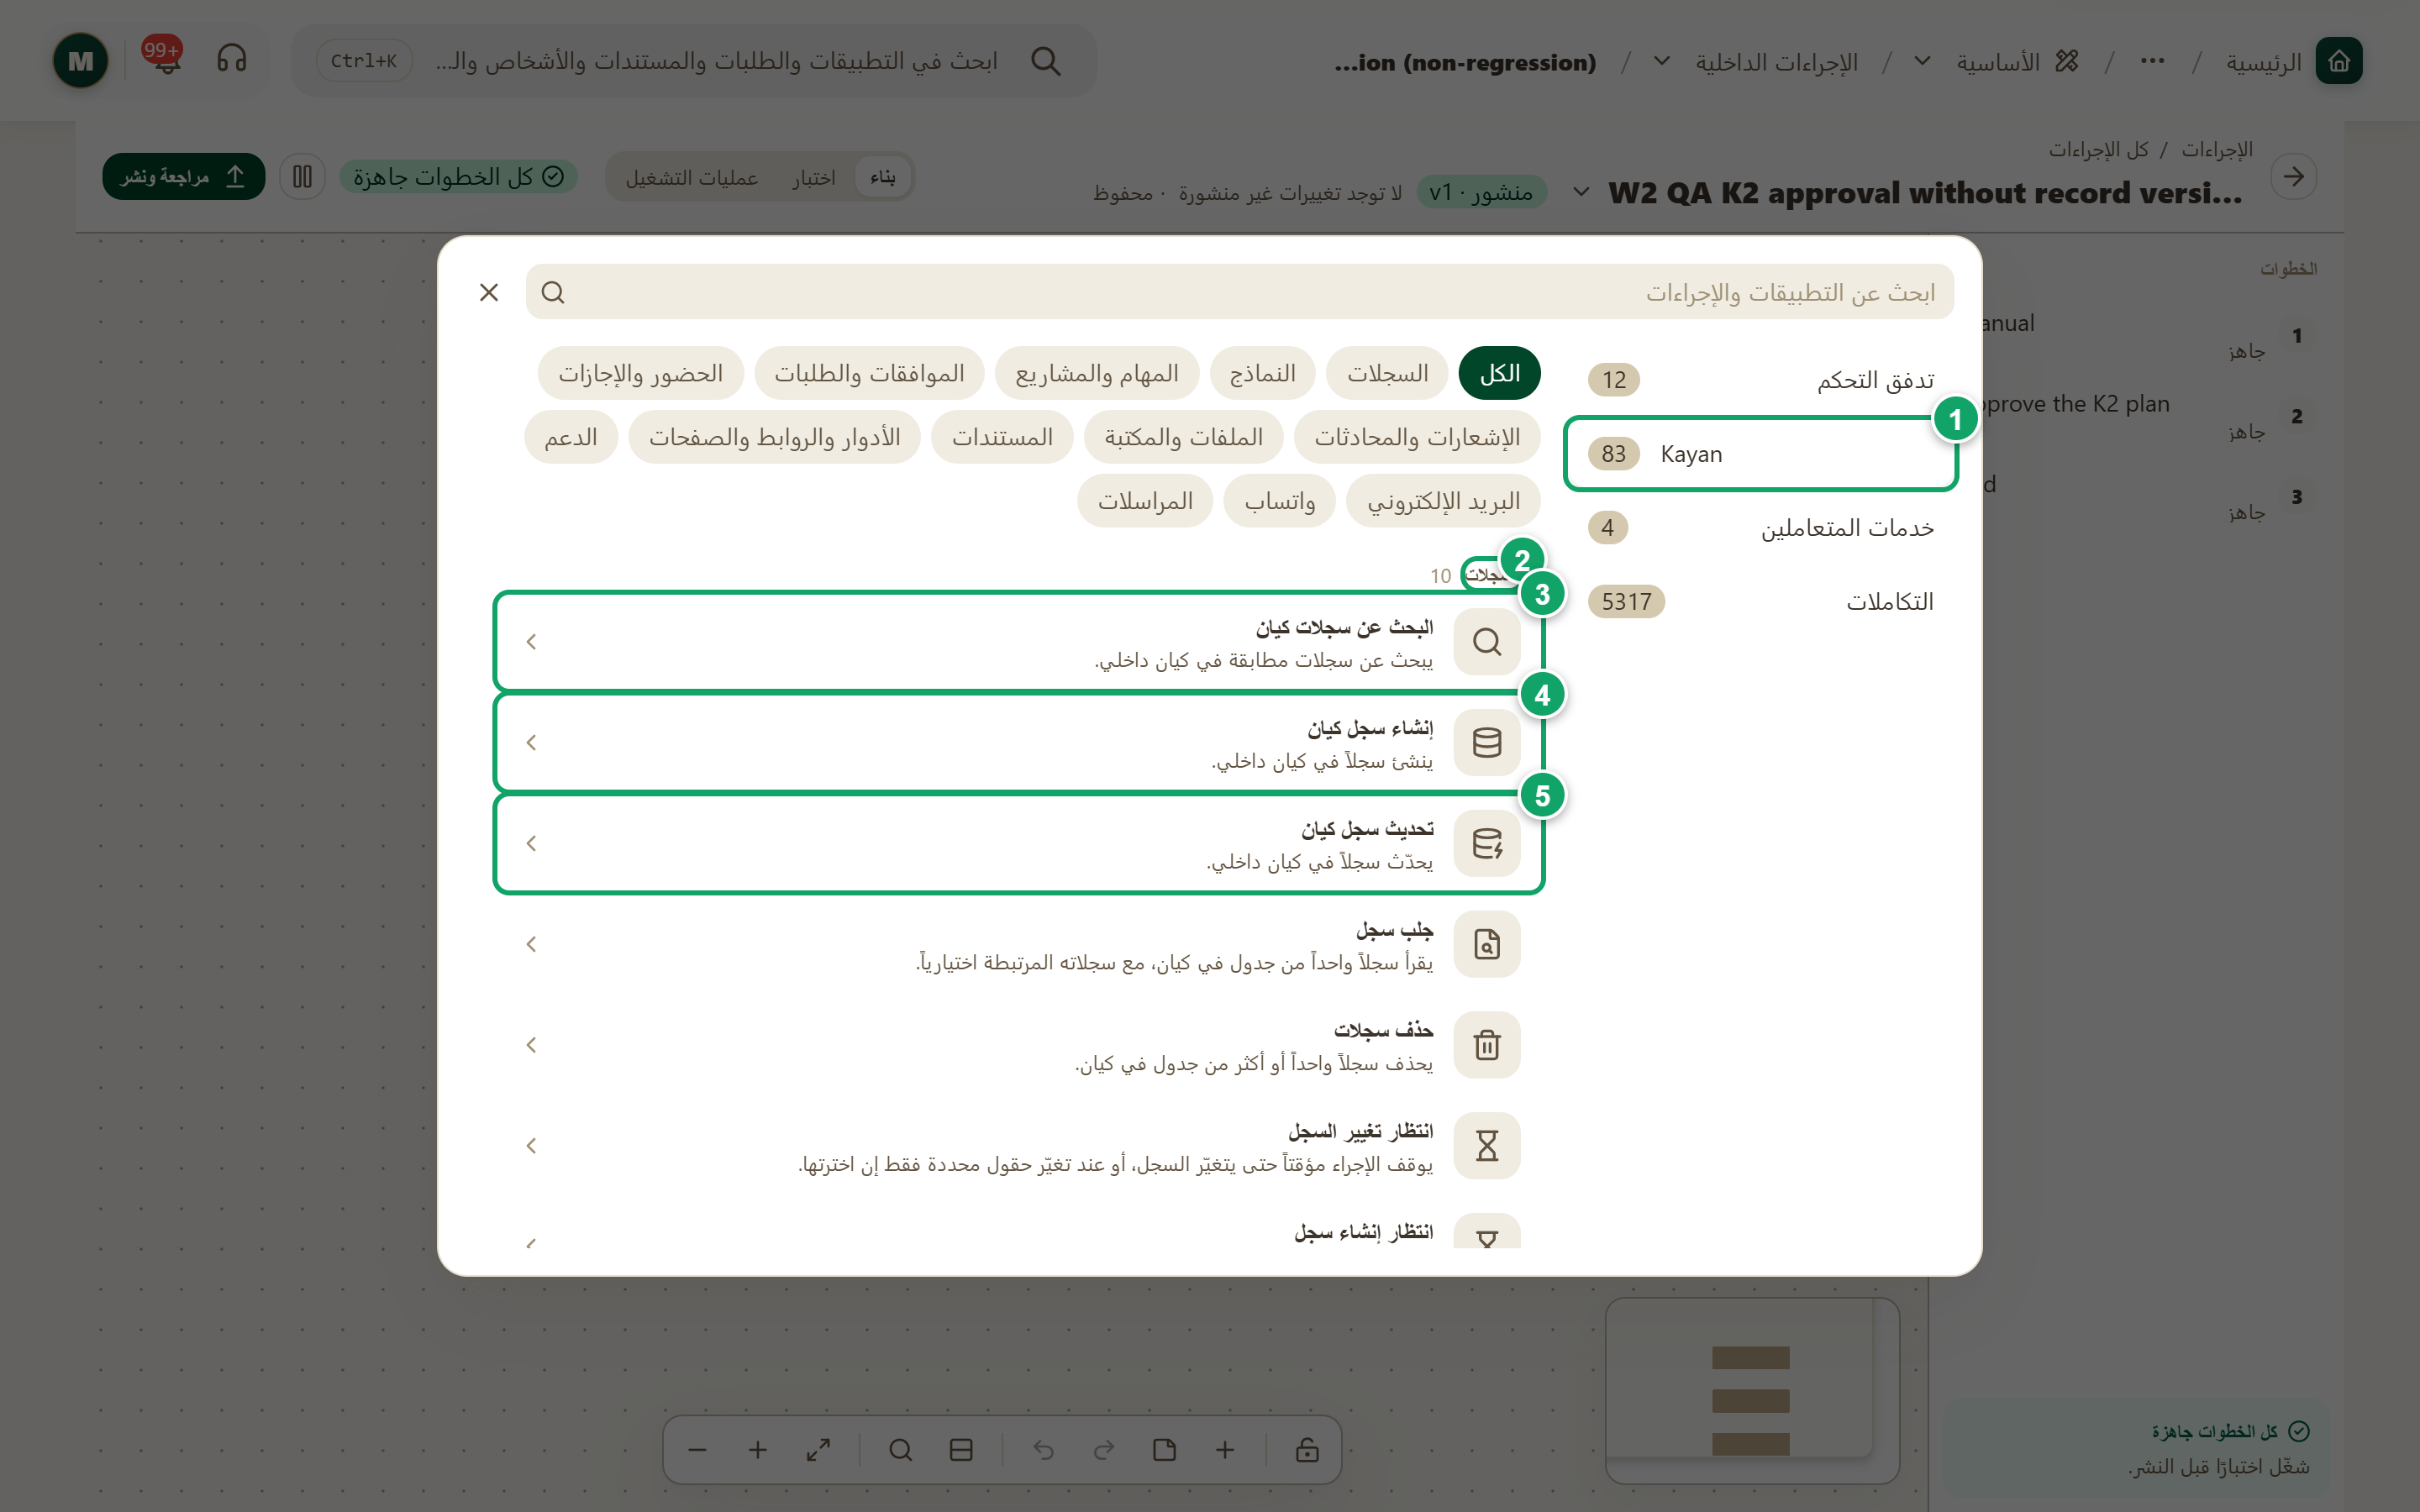
\includegraphics[width=0.95\linewidth,height=0.72\textheight,keepaspectratio]{figures/screens/ch06-isop-records-ar.png}
\caption{قسم «السجلات» في فئة «Kayan»}
\label{fig:builder-isop-records-screen}
\shotnote{تعرض الصورة فئة «Kayan» في قائمة الخطوات، وفيها أزرار الأقسام ثم خطوات قسم «السجلات». ويبيّن ذلك أن خطوات السجلات والنماذج كلها في فئة واحدة تصل إليها بزر القسم بدلاً من التمرير الطويل. ① «Kayan»: فئة خطوات النظام. ② «السجلات»: القسم الذي يجمع خطوات السجلات. ③ «البحث عن سجلات كيان»: يعيد السجلات المطابقة لشروطك. ④ «إنشاء سجل كيان»: ينشئ سجلاً جديداً. ⑤ «تحديث سجل كيان»: يعدّل حقول سجل قائم.}
\end{figure}

\begin{table}[H]
\centering
\caption{خطوات السجلات}
\label{tab:builder-isop-records-steps}
\begin{tabularx}{\linewidth}{R{3.6cm} Y}
\rcHeaderRow
\thh{الخطوة} & \thh{ما تفعله وأهم حقولها}\\
البحث عن سجلات كيان & تعيد السجلات المطابقة لشروطك في «الكيان» المختار، مع الحقول التي تحددها وعدد أقصى بين 1 و1000.\\
إنشاء سجل كيان & تُنشئ سجلاً وتملأ «قيم الحقول» «حقل بحقل» أو «كائن كامل». ويحدد «إذا وُجد سجل مطابق» ما يحدث عند التكرار: «إيقاف بخطأ» أو «تخطٍّ» أو «استخدام الموجود».\\
تحديث سجل كيان & تحدّث حقول «السجل» الذي تختاره أو الذي يأتي من المشغّل.\\
جلب سجل، حذف سجلات & تقرأ سجلاً واحداً لتستخدم قيمه، أو تحذف سجلات.\\
انتظار تغيير السجل، انتظار إنشاء سجل & توقف الإجراء حتى يتغير سجل أو يُنشأ سجل يطابق الشرط.\\
تنفيذ إجراء كيان & تنفّذ إجراءً معرّفاً على نوع السجلات، مثل الانتقال إلى حالة.\\
\end{tabularx}
\end{table}

\begin{table}[H]
\centering
\caption{خطوات النماذج}
\label{tab:builder-isop-records-forms}
\begin{tabularx}{\linewidth}{R{3.6cm} Y}
\rcHeaderRow
\thh{الخطوة} & \thh{ما تفعله}\\
طلب نموذج & تطلب من الأعضاء المحددين في «المستلمون» تعبئة «النموذج» المختار، مع «تاريخ الاستحقاق» و«انتظار الاكتمال» و«مهلة الانتظار».\\
بدء جلسة نموذج & تبدأ جلسة تعبئة جديدة لنموذج.\\
جلب إرسال نموذج، البحث عن إرسالات النماذج & تقرأ ما أرسله الأعضاء لتستخدمه في الخطوات التالية.\\
حفظ النموذج بصيغة \en{PDF} & تحفظ الإرسال ملفاً بصيغة \en{PDF}.\\
\end{tabularx}
\end{table}

\begin{figure}[H]
\centering
\begin{tikzpicture}[node distance=0.5cm]
\node[stepBox] (a) {\RL{اختيار الكيان}};
\node[stepBox,below=of a] (b) {\RL{اختيار السجل أو الشروط}};
\node[stepBox,below=of b] (c) {\RL{تعيين قيم الحقول}};
\node[stepBox,below=of c] (d) {\RL{إضافة الحقول المطلوبة}};
\node[stepBox,below=of d] (e) {\RL{اختبار الخطوة}};
\draw[flowsTo] (a) -- (b);
\draw[flowsTo] (b) -- (c);
\draw[flowsTo] (c) -- (d);
\draw[flowsTo] (d) -- (e);
\end{tikzpicture}
\rclegend
\caption{إعداد خطوة سجل}
\label{fig:builder-isop-records-flow}
\shotnote{يبدأ المخطط باختيار الكيان لأن الحقول المتاحة تُحمَّل منه، فلا تستطيع اختيار السجل أو القيم قبله. ويضع إضافة الحقول المطلوبة قبل الاختبار، لأن الخطوة لا تكتمل حتى تعيّن قيماً لكل الحقول الإلزامية في نوع السجلات.}
\end{figure}

\subsection{خطوات العمل والتحقق}
\begin{enumerate}
\item أضف الخطوة من قسم «السجلات»، واختر «الكيان».
\item في خطوة التحديث، اختر «السجل»، أو استخدم السجل الذي جاء من المشغّل بدلاً من سجل ثابت.
\item في «قيم الحقول»، اضغط «إضافة قيمة» واختر الحقل ثم اكتب قيمته أو أدرجها من خطوة سابقة.
\item اضغط «إضافة الحقول المطلوبة» إذا ظهر، حتى تغطي كل الحقول الإلزامية.
\end{enumerate}

\textbf{تحقق ومعالجة المشكلة:} يجب أن يختفي من الخطوة تنبيه «عيّن قيمًا للحقول المطلوبة». فإذا ظهر «لا توجد حقول قابلة للكتابة لهذه العملية»، فتحقق من صلاحياتك على نوع السجلات. وإذا تجاوزت الخطوة حداً على السجلات، فاكتب «التبرير عند تجاوز حدّ» إن كان الحد يسمح بالتجاوز، وإلا توقف التشغيل.

\clearpage
\section{خطوات المهام والموافقات والإشعارات والمستندات}
\label{sec:builder-feature-isop-people}

هذه الخطوات تشرك الأشخاص في الإجراء: تُنشئ مهمة لعضو، أو تطلب موافقة أو توقيعاً، أو ترسل إشعاراً، أو تُنشئ مستنداً من قالب. وبعضها ينتظر رد الشخص قبل أن يتابع، فيبقى التشغيل في حالة «بانتظار استجابة» حتى يصل الرد أو تنتهي المهلة.

\textbf{المسار ومن يستخدمه:} المحرر ← زر الإضافة ← \en{Kayan} ← «المهام والمشاريع» أو «الموافقات والطلبات» أو «الإشعارات والمحادثات» أو «المستندات». يستخدمها من يبني الإجراء.

\begin{rcnote}[مثال: شركة الأفق]
يضيف المسؤول «طلب موافقة» (⑤) بعنوان «اعتماد زيارة فرع حلب» وتكون سارة الخطيب في مرحلته الوحيدة. وبعد موافقتها تُنشئ خطوة «إنشاء مهمة» مهمة «تجهيز الزيارة» وتضيف عمر حداد إلى حقل «المكلّفون».
\end{rcnote}

\begin{figure}[H]
\centering
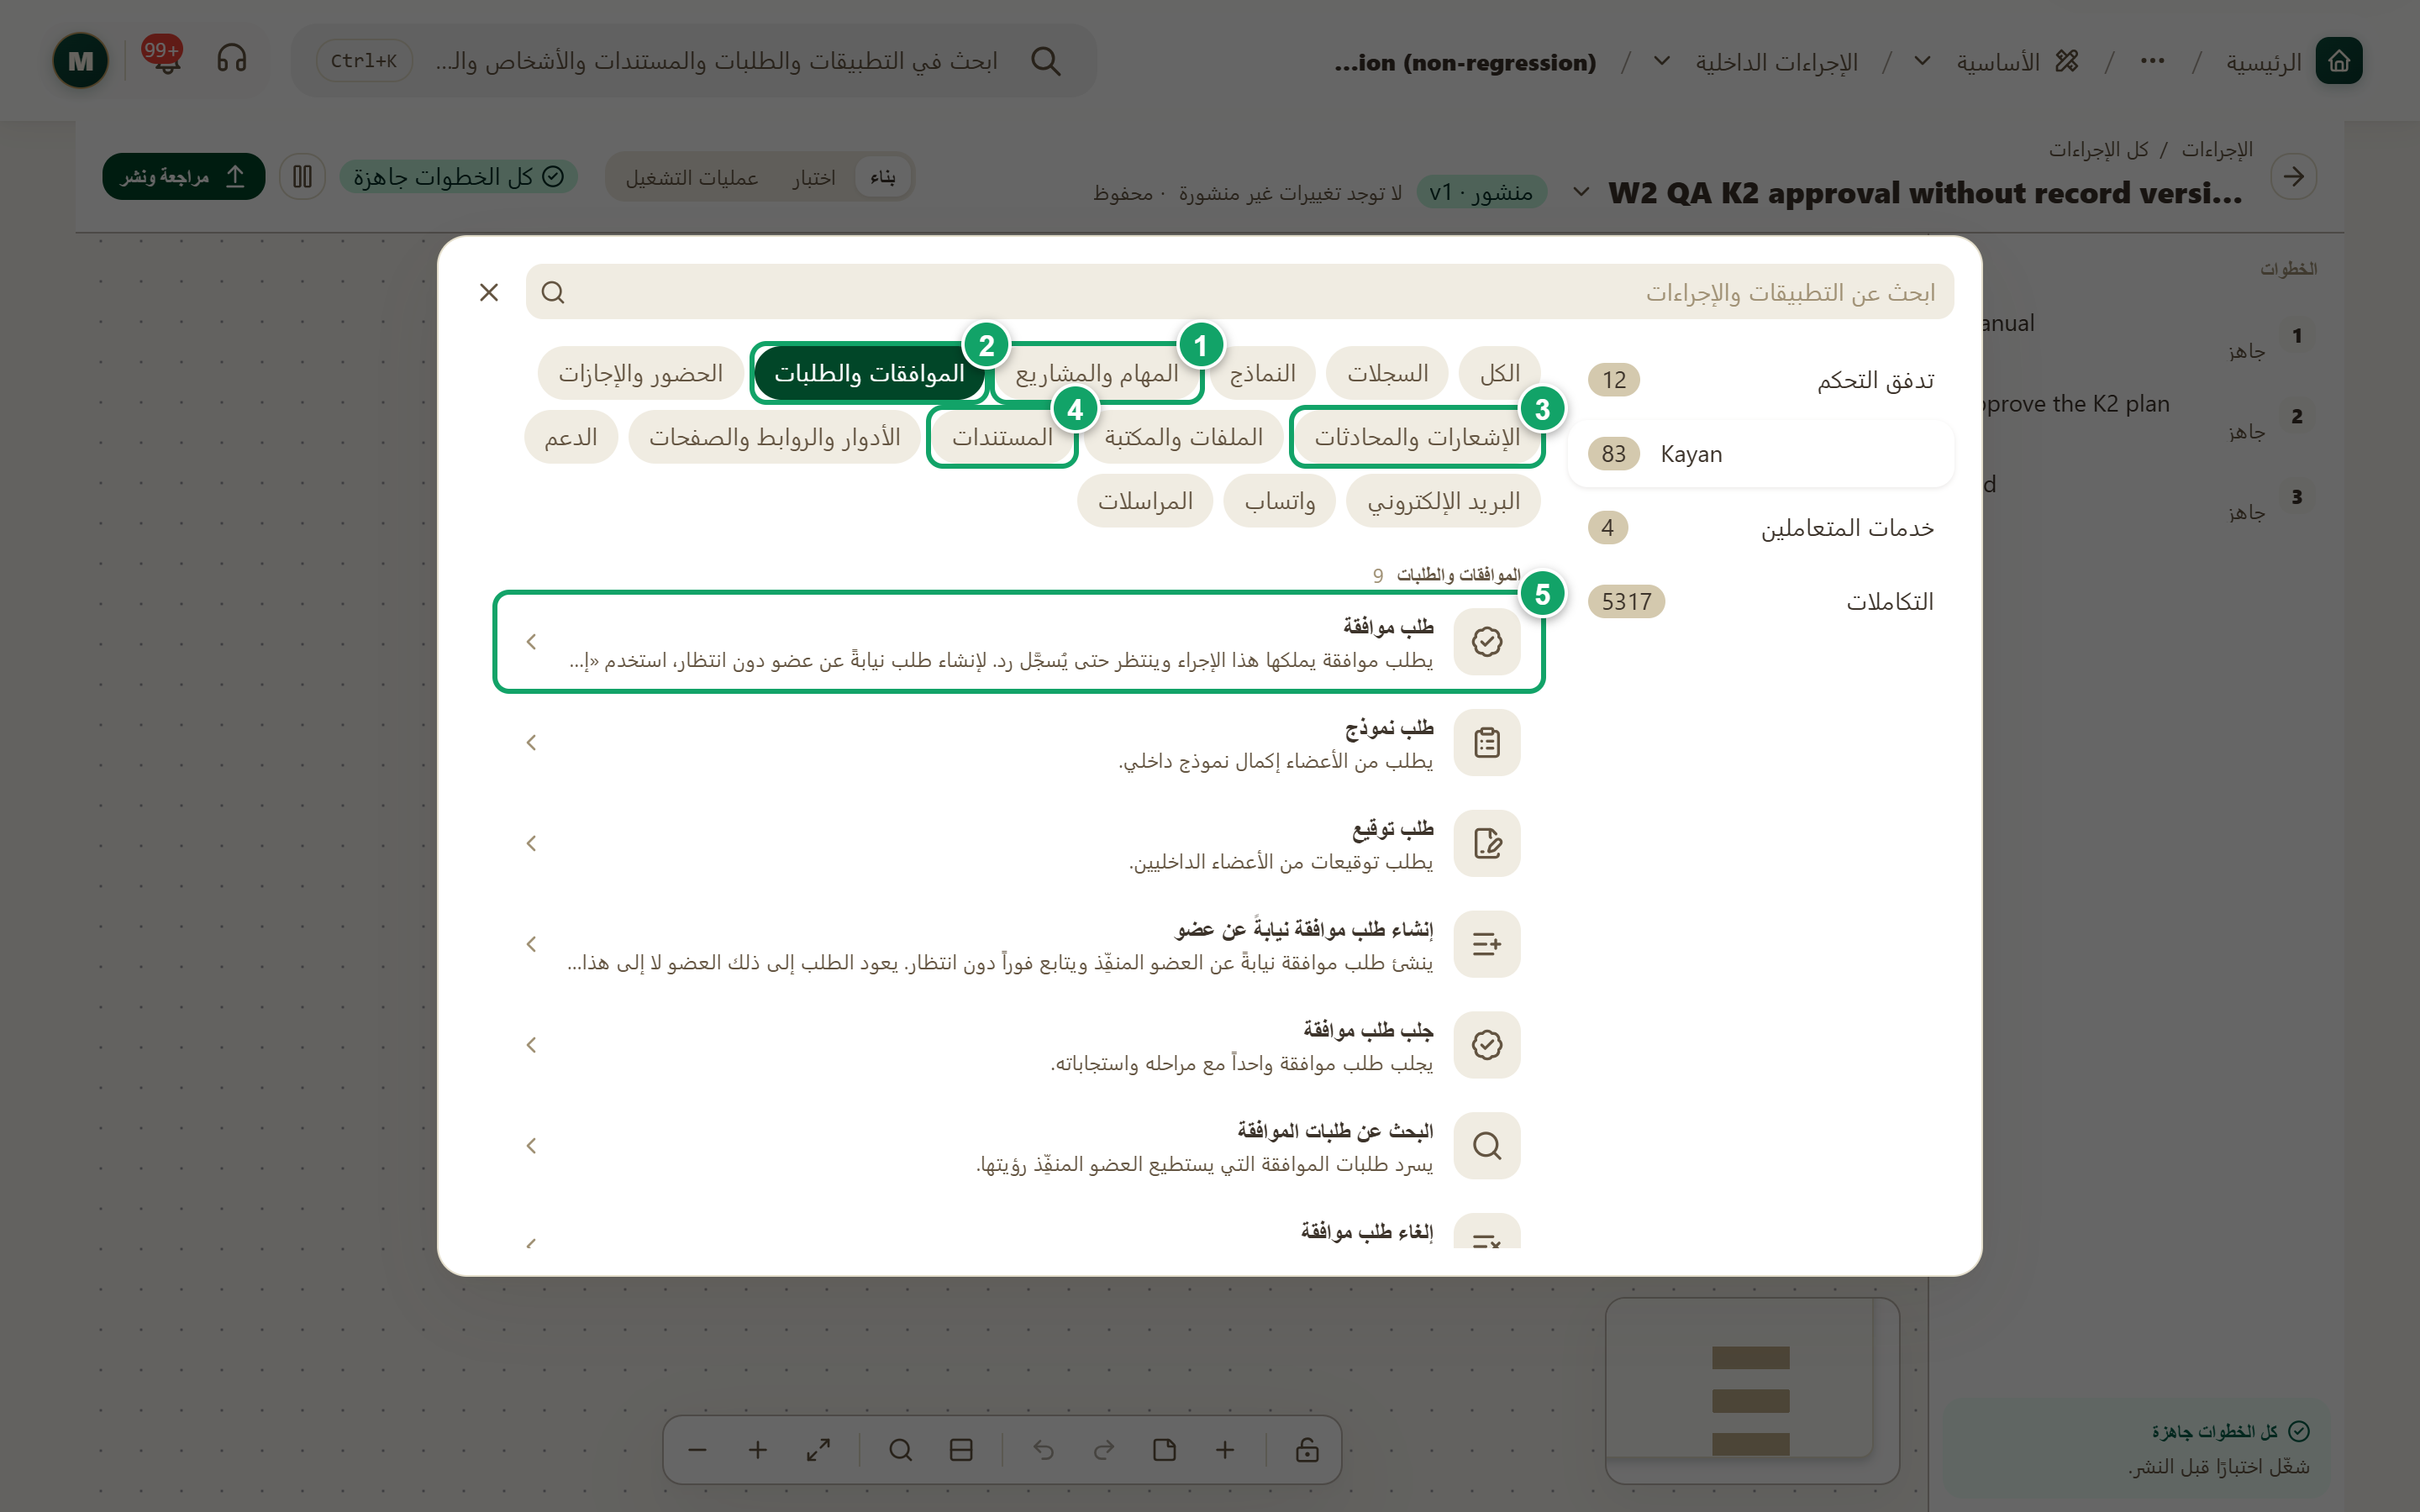
\includegraphics[width=0.95\linewidth,height=0.72\textheight,keepaspectratio]{figures/screens/ch06-isop-people-ar.png}
\caption{قسم «الموافقات والطلبات» في فئة «Kayan»}
\label{fig:builder-isop-people-screen}
\shotnote{تعرض الصورة قائمة الخطوات بعد اختيار قسم «الموافقات والطلبات»، وفيه خطوات طلب الموافقة والنموذج والتوقيع وما يتصل بها. ومن أزرار الأقسام نفسها تصل إلى خطوات المهام والإشعارات والمستندات التي تشرحها هذه الصفحة. ① «المهام والمشاريع»: خطوات إنشاء المهام وتحديثها. ② «الموافقات والطلبات»: القسم المعروض في الصورة. ③ «الإشعارات والمحادثات»: خطوات إرسال الإشعارات. ④ «المستندات»: توليد مستند أو جدول بيانات. ⑤ «طلب موافقة»: الخطوة التي تطلب الموافقة وتنتظر الرد.}
\end{figure}

\begin{table}[H]
\centering
\caption{أهم الخطوات وحقولها}
\label{tab:builder-isop-people-steps}
\begin{tabularx}{\linewidth}{R{3.6cm} Y}
\rcHeaderRow
\thh{الخطوة} & \thh{ما تفعله وأهم حقولها}\\
إنشاء مهمة & تُنشئ مهمة داخلية: «عنوان المهمة» و«تفاصيل المهمة» و«المكلّفون» و«الأولوية» و«تاريخ الاستحقاق»، ويمكن تحديد «نوع المهمة» و«مالك المهمة».\\
طلب موافقة & يطلب موافقة وينتظر الرد: «عنوان الموافقة» و«مراحل الموافقة» بمعتمد واحد على الأقل في كل مرحلة، و«إجراءات الطلب»، و«انتظار الاكتمال» مع «المهلة الزمنية» التي تبدأ بثلاثين يوماً.\\
طلب توقيع & يطلب توقيعات الأعضاء وفق «قواعد التوقيع»، مع تعليمات ومرفقات من المكتبة.\\
إرسال إشعار & يرسل إشعاراً إلى «المستلمون» أو إلى «محدِّدات الأعضاء» مثل الأدوار والأقسام، مع «عنوان الرسالة» و«محتوى الرسالة» ورابط اختياري.\\
خطوات المهام الأخرى & «تحديث مهمة» و«تنفيذ إجراء على مهمة» و«انتظار إجراء على مهمة» و«إضافة تعليق على مهمة».\\
خطوات الموافقات الأخرى & «إرسال تذكير بالموافقة» و«إلغاء طلب موافقة» و«إنشاء طلب موافقة نيابةً عن عضو» الذي لا ينتظر الرد.\\
المستندات & «إنشاء مستند من قالب» و«إنشاء جدول بيانات».\\
\end{tabularx}
\end{table}

\subsection{إجراءات الطلب}

تأتي خطوة «طلب موافقة» بإجراءين جاهزين: الموافقة، وتطلب توقيعاً ويكون التعليق فيها اختيارياً؛ وطلب التغييرات، ويكون التعليق فيها إلزامياً وتنهي الطلب. ولكل إجراء نتيجة تحفظها الخطوة، فتستطيع أن تقرأها في «تفرّع شرطي» بعدها لتختار المسار.

\begin{figure}[H]
\centering
\begin{tikzpicture}[node distance=0.5cm]
\node[stepBox] (a) {\RL{طلب موافقة}};
\node[stepBox,below=of a] (b) {\RL{بانتظار رد المعتمد}};
\node[stepBox,below=of b] (c) {\RL{تفرّع حسب النتيجة}};
\node[stepBox,below=of c] (d) {\RL{إنشاء مهمة}};
\node[stepBox,below=of d] (e) {\RL{إرسال إشعار}};
\draw[flowsTo] (a) -- (b);
\draw[flowsTo] (b) -- (c);
\draw[flowsTo] (c) -- (d);
\draw[flowsTo] (d) -- (e);
\end{tikzpicture}
\rclegend
\caption{مسار يشرك الأشخاص}
\label{fig:builder-isop-people-flow}
\shotnote{يبيّن المخطط أن الموافقة تفصل الإجراء إلى ما قبل الرد وما بعده، فلا تُنشأ المهمة إلا بعد أن يقرر المعتمد. لذلك يأتي القرار بعد طلب الموافقة مباشرة، ليذهب كل رد إلى المسار المناسب له.}
\end{figure}

\subsection{خطوات العمل والتحقق}
\begin{enumerate}
\item أضف «طلب موافقة»، واكتب «عنوان الموافقة»، ثم اضغط «إضافة مرحلة» واختر المعتمدين.
\item راجع «إجراءات الطلب»، وأبقِ «انتظار الاكتمال» مفعّلاً إذا كانت الخطوات التالية تعتمد على الرد.
\item أضف بعده «تفرّع شرطي» يقرأ نتيجة الموافقة.
\item أضف «إنشاء مهمة» في مسار الموافقة، واكتب «عنوان المهمة»، ثم اختر الأعضاء في «المكلّفون».
\end{enumerate}

\textbf{تحقق ومعالجة المشكلة:} يجب ألا تحمل الخطوات شارة «يحتاج إلى تهيئة». فإذا ظهر «مطلوب معتمد واحد على الأقل»، فأضف معتمداً إلى كل مرحلة. وإذا بقي التشغيل منتظراً طويلاً، فأضف بعد الخطوة «إرسال تذكير بالموافقة»، أو قصّر «المهلة الزمنية».

\clearpage
\section{إعداد الخطوة: المدخلات والبيانات والتعبيرات}
\label{sec:builder-feature-isop-inspector}

عندما تضغط خطوة على اللوحة تُفتح لوحة إعدادها بجانب اللوحة الرئيسية. وفيها تعدّل اسم الخطوة، وتملأ مدخلاتها، وتختار مصدر كل قيمة: قيمة تكتبها بنفسك، أو بيانات من المشغّل أو من خطوة سابقة، أو تعبيراً يحسب القيمة. وتُحفظ التغييرات تلقائياً.

\textbf{المسار ومن يستخدمه:} المحرر ← اضغط الخطوة ← لوحة الإعداد. يستخدمها من يبني الإجراء.

\begin{rcnote}[مثال: شركة الأفق]
في خطوة «إنشاء مهمة»، يضغط المسؤول «إدراج بيانات» (②) بجانب «عنوان المهمة»، ويختار رقم الطلب من بيانات المشغّل، فيصبح العنوان «تجهيز الزيارة \en{HZN-VR-0001}» لكل طلب بحسب رقمه.
\end{rcnote}

\begin{figure}[H]
\centering
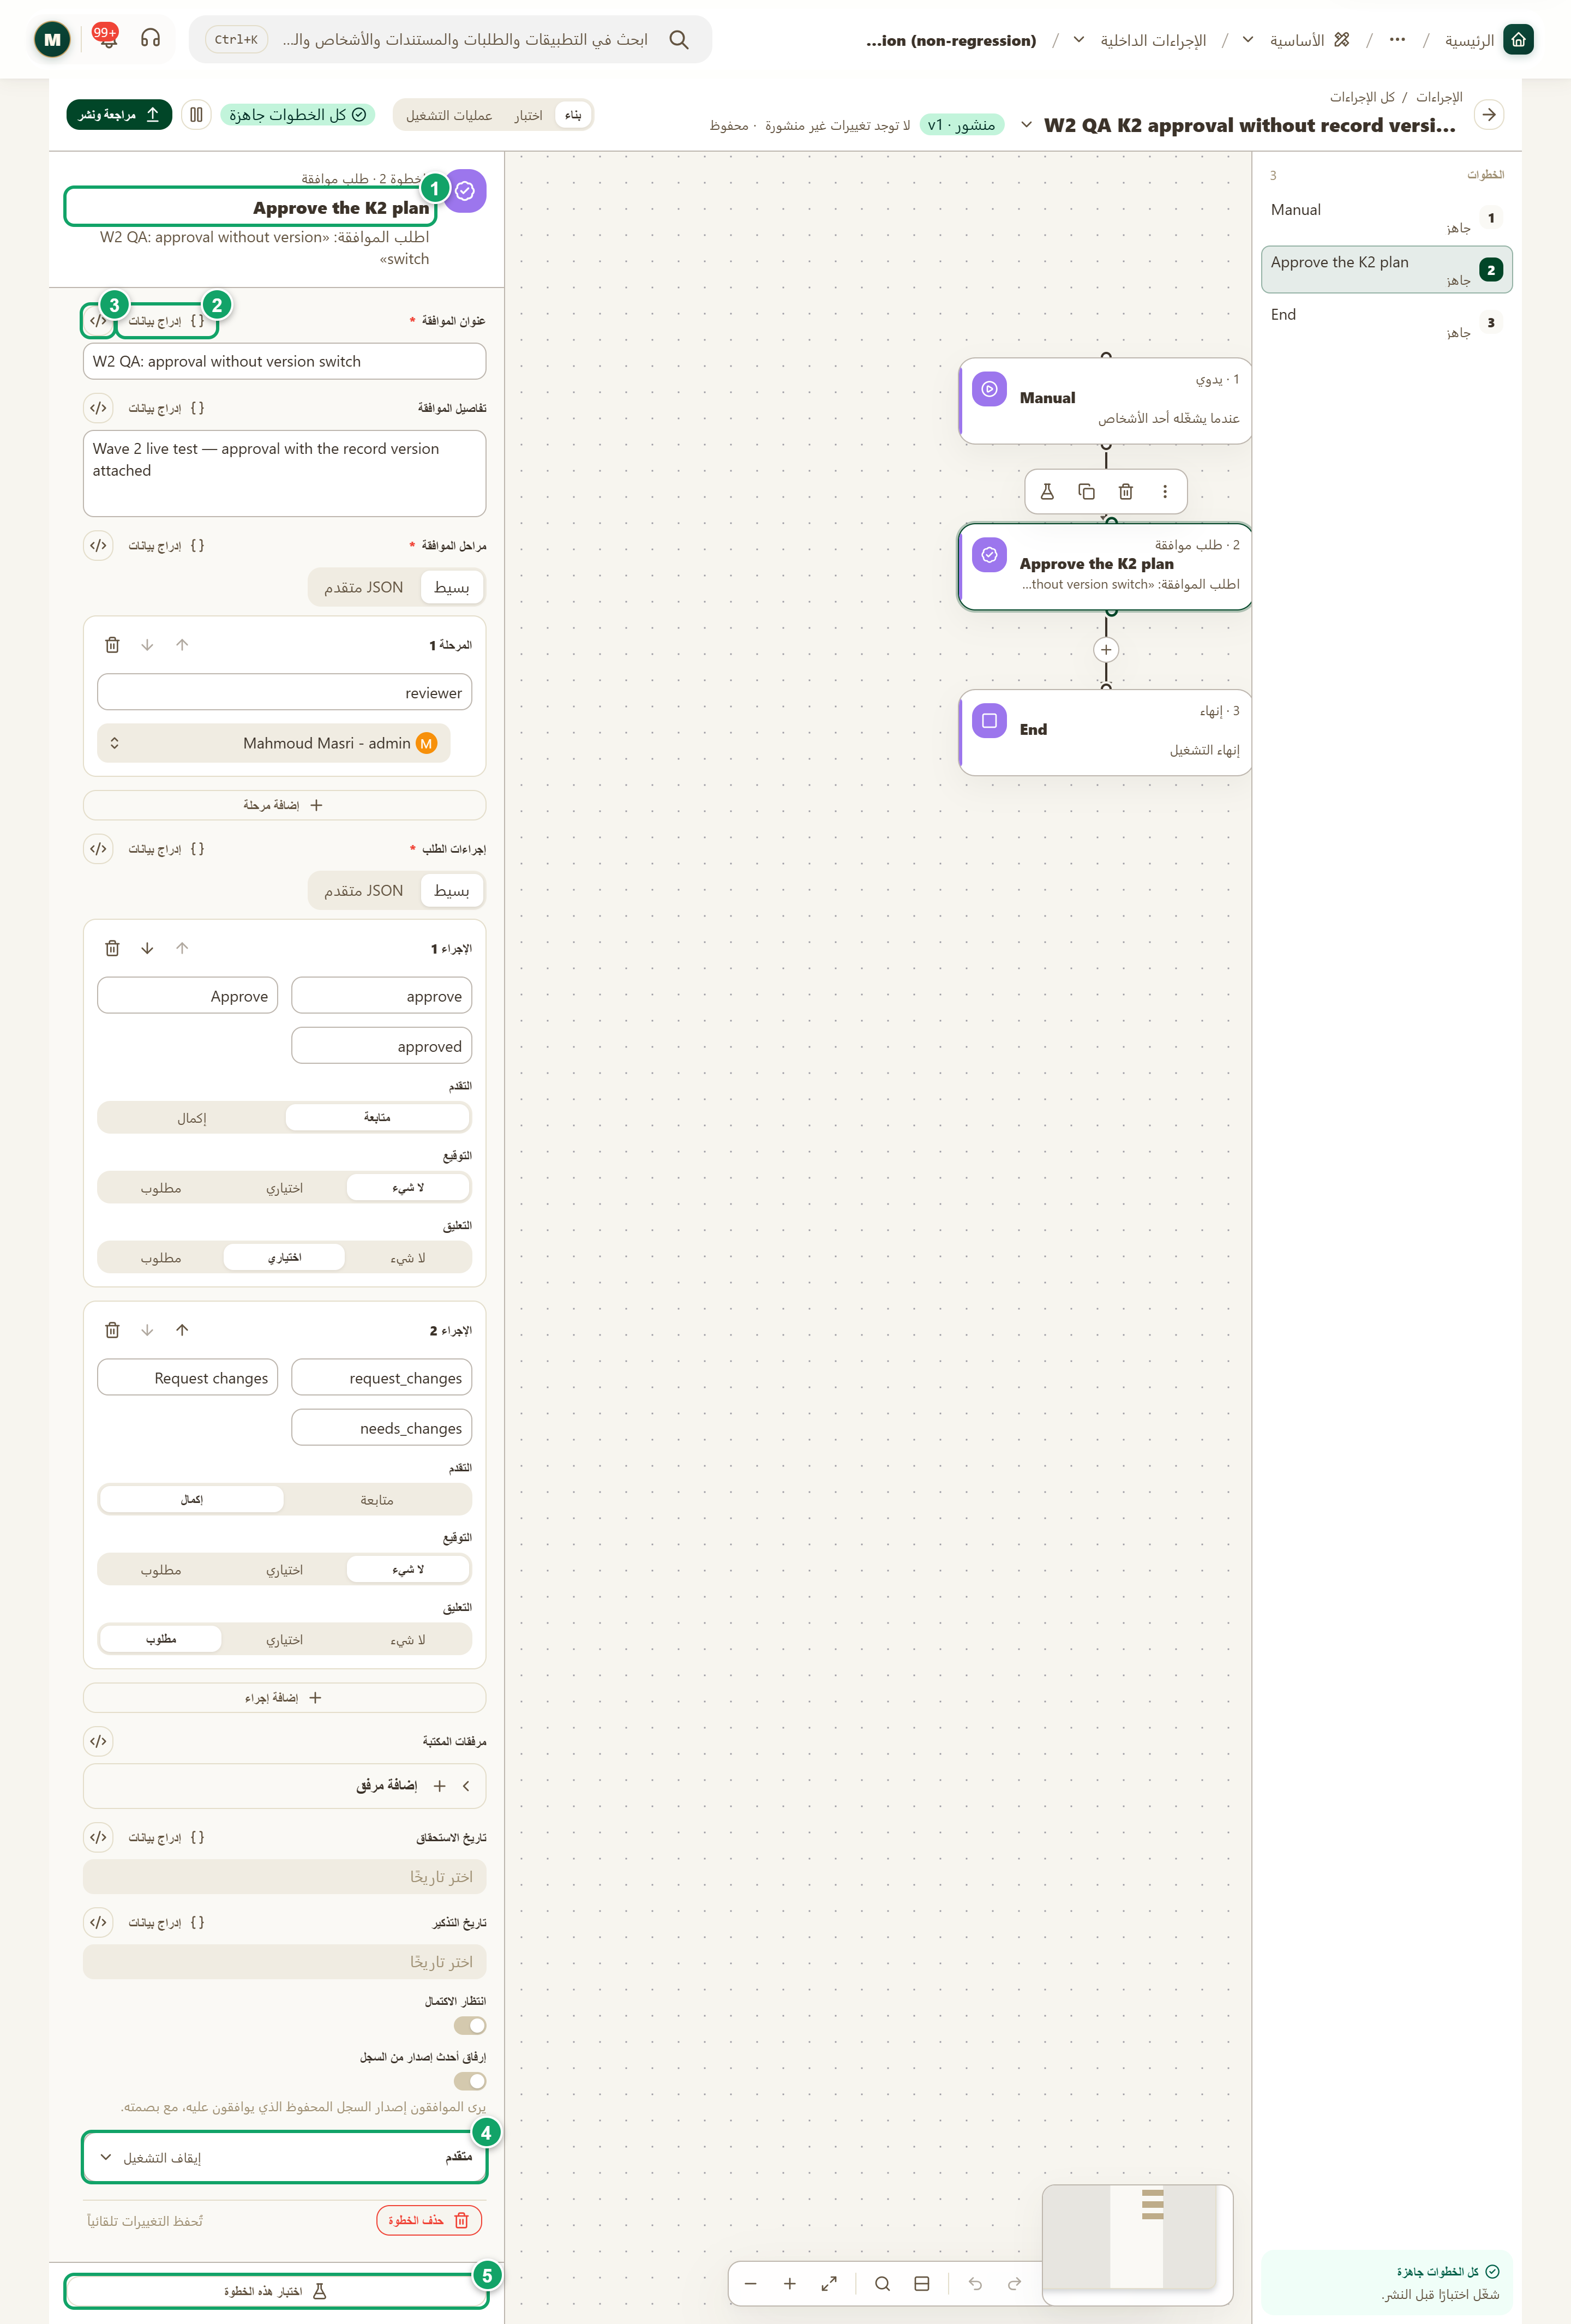
\includegraphics[width=0.95\linewidth,height=0.72\textheight,keepaspectratio]{figures/screens/ch06-isop-inspector-ar.png}
\caption{لوحة إعداد خطوة «طلب موافقة»}
\label{fig:builder-isop-inspector-screen}
\shotnote{تعرض الصورة لوحة إعداد خطوة «طلب موافقة» في الإجراء الاختباري، وفيها حقول الخطوة كاملة من العنوان إلى «متقدم». ويتكرر بجانب كل حقل الزران نفسهما، فتعرف أن أي قيمة يمكن أن تُكتب أو تُدرج أو تُحسب. ① اسم الخطوة: تعدّله بالضغط عليه. ② «إدراج بيانات»: يدرج قيمة من المشغّل أو من خطوة سابقة. ③ زر التعبير: يحوّل الحقل إلى تعبير تكتبه. ④ «متقدم»: الوصف والاسم المرجعي وما يحدث عند الفشل. ⑤ «اختبار هذه الخطوة»: يشغّل الخطوة وحدها.}
\end{figure}

\begin{table}[H]
\centering
\caption{أجزاء لوحة إعداد الخطوة}
\label{tab:builder-isop-inspector-parts}
\begin{tabularx}{\linewidth}{R{3.6cm} Y}
\rcHeaderRow
\thh{الجزء} & \thh{ما يقدمه}\\
الرأس & اسم الخطوة، وتعدّله بالضغط عليه، وتحته رقمها ونوعها مثل «الخطوة 3 · طلب موافقة».\\
المدخلات & حقول الخطوة، والمطلوب منها معلَّم. وتظهر المشكلات تحت الحقل الناقص مباشرة.\\
إدراج بيانات & يفتح قائمة بالبيانات المتاحة للحقل: المشغّل، والخطوات السابقة، والعنصر الحالي داخل «لكل عنصر»، و«المتغيرات». وتظهر بجانب كل حقل قيمة نموذجية من آخر اختبار.\\
زر التعبير & يحوّل الحقل إلى تعبير تكتبه بنفسك عندما تحتاج إلى حساب أو صيغة.\\
متقدم & «إذا فشلت هذه الخطوة» و«تخطي هذه الخطوة» و«الوصف» و«الاسم المرجعي» الذي تستخدمه الصيغ.\\
التذييل & «اختبار هذه الخطوة» و«حذف الخطوة»، مع عبارة «تُحفظ التغييرات تلقائياً».\\
\end{tabularx}
\end{table}

\begin{rcwarn}[الاسم المرجعي]
تشير الصيغ إلى الخطوة باسمها المرجعي، لذلك اجعله مقروءاً بأحرف إنجليزية صغيرة وأرقام وشرطات سفلية. وعند تغييره يحدّث النظام كل صيغة تشير إلى الخطوة، لكنه يرفض اسماً تستخدمه خطوة أخرى.
\end{rcwarn}

\begin{figure}[H]
\centering
\begin{tikzpicture}[node distance=0.5cm]
\node[stepBox] (a) {\RL{اختيار الخطوة}};
\node[stepBox,below=of a] (b) {\RL{تعبئة المدخلات}};
\node[stepBox,below=of b] (c) {\RL{إدراج بيانات سابقة}};
\node[stepBox,below=of c] (d) {\RL{كتابة تعبير عند الحاجة}};
\node[stepBox,below=of d] (e) {\RL{اختبار هذه الخطوة}};
\draw[flowsTo] (a) -- (b);
\draw[flowsTo] (b) -- (c);
\draw[flowsTo] (c) -- (d);
\draw[flowsTo] (d) -- (e);
\end{tikzpicture}
\rclegend
\caption{من الحقل الفارغ إلى قيمة صحيحة}
\label{fig:builder-isop-inspector-flow}
\shotnote{يرتب المخطط مصادر القيمة من الأبسط إلى الأعقد: تكتب القيمة، فإن كانت تتغير مع كل تشغيل أدرجتها من بيانات سابقة، وتلجأ إلى التعبير عند الحاجة إلى حساب. ويختم باختبار الخطوة لترى القيمة الفعلية التي استلمتها.}
\end{figure}

\subsection{خطوات العمل والتحقق}
\begin{enumerate}
\item اضغط الخطوة على اللوحة أو في قائمة «الخطوات».
\item املأ الحقول المطلوبة، واضغط «إدراج بيانات» بجانب أي حقل تأتي قيمته من المشغّل أو من خطوة سابقة.
\item ابحث في «ابحث في الحقول» عن الحقل الذي تريده، ثم اضغطه ليُدرج في مكانه.
\item افتح «متقدم» إذا أردت كتابة وصف للخطوة أو تعديل اسمها المرجعي.
\end{enumerate}

\textbf{تحقق ومعالجة المشكلة:} يجب أن تظهر البيانات المدرجة داخل الحقل مرجعاً مميزاً، وأن تختفي شارة «يحتاج إلى تهيئة». فإذا ظهر في قائمة البيانات «شغّل اختبارًا لرؤية قيم نموذجية هنا»، فشغّل اختباراً أولاً لترى القيم. وإذا نبّهك المحرر إلى مرجع بيانات غير مكتمل في حقل، فاحذف المرجع وأدرجه من جديد.

\clearpage
\section{معالجة الأخطاء وتخطي الخطوات}
\label{sec:builder-feature-isop-errors}

قد تفشل خطوة لأن خدمة خارجية لم تستجب، أو لأن سجلاً لم يعد موجوداً. ويحدد قسم «معالجة الأخطاء» ما يحدث عندئذ: أن يتوقف التشغيل كله، أو أن يتابع في مسار بديل تبنيه أنت. وتستطيع أيضاً أن تطلب إعادة المحاولة قبل اعتبار الخطوة فاشلة، أو أن تُبقي الخطوة في المسار دون تشغيلها مؤقتاً.

\textbf{المسار ومن يستخدمه:} المحرر ← اضغط الخطوة ← «متقدم» ← «إذا فشلت هذه الخطوة». يستخدمه من يبني الإجراء. ولا يظهر الخياران لخطوات المشغّل و«تفرّع شرطي» و«إنهاء».

\begin{rcnote}[مثال: شركة الأفق]
يفعّل المسؤول «إعادة المحاولة قبل الاستسلام» في خطوة «إرسال إشعار» إلى عمر حداد، ويختار «اتباع مسار الفشل» (③) ليرسل في مسار الفشل إشعاراً بديلاً إلى سارة الخطيب.
\end{rcnote}

\begin{figure}[H]
\centering
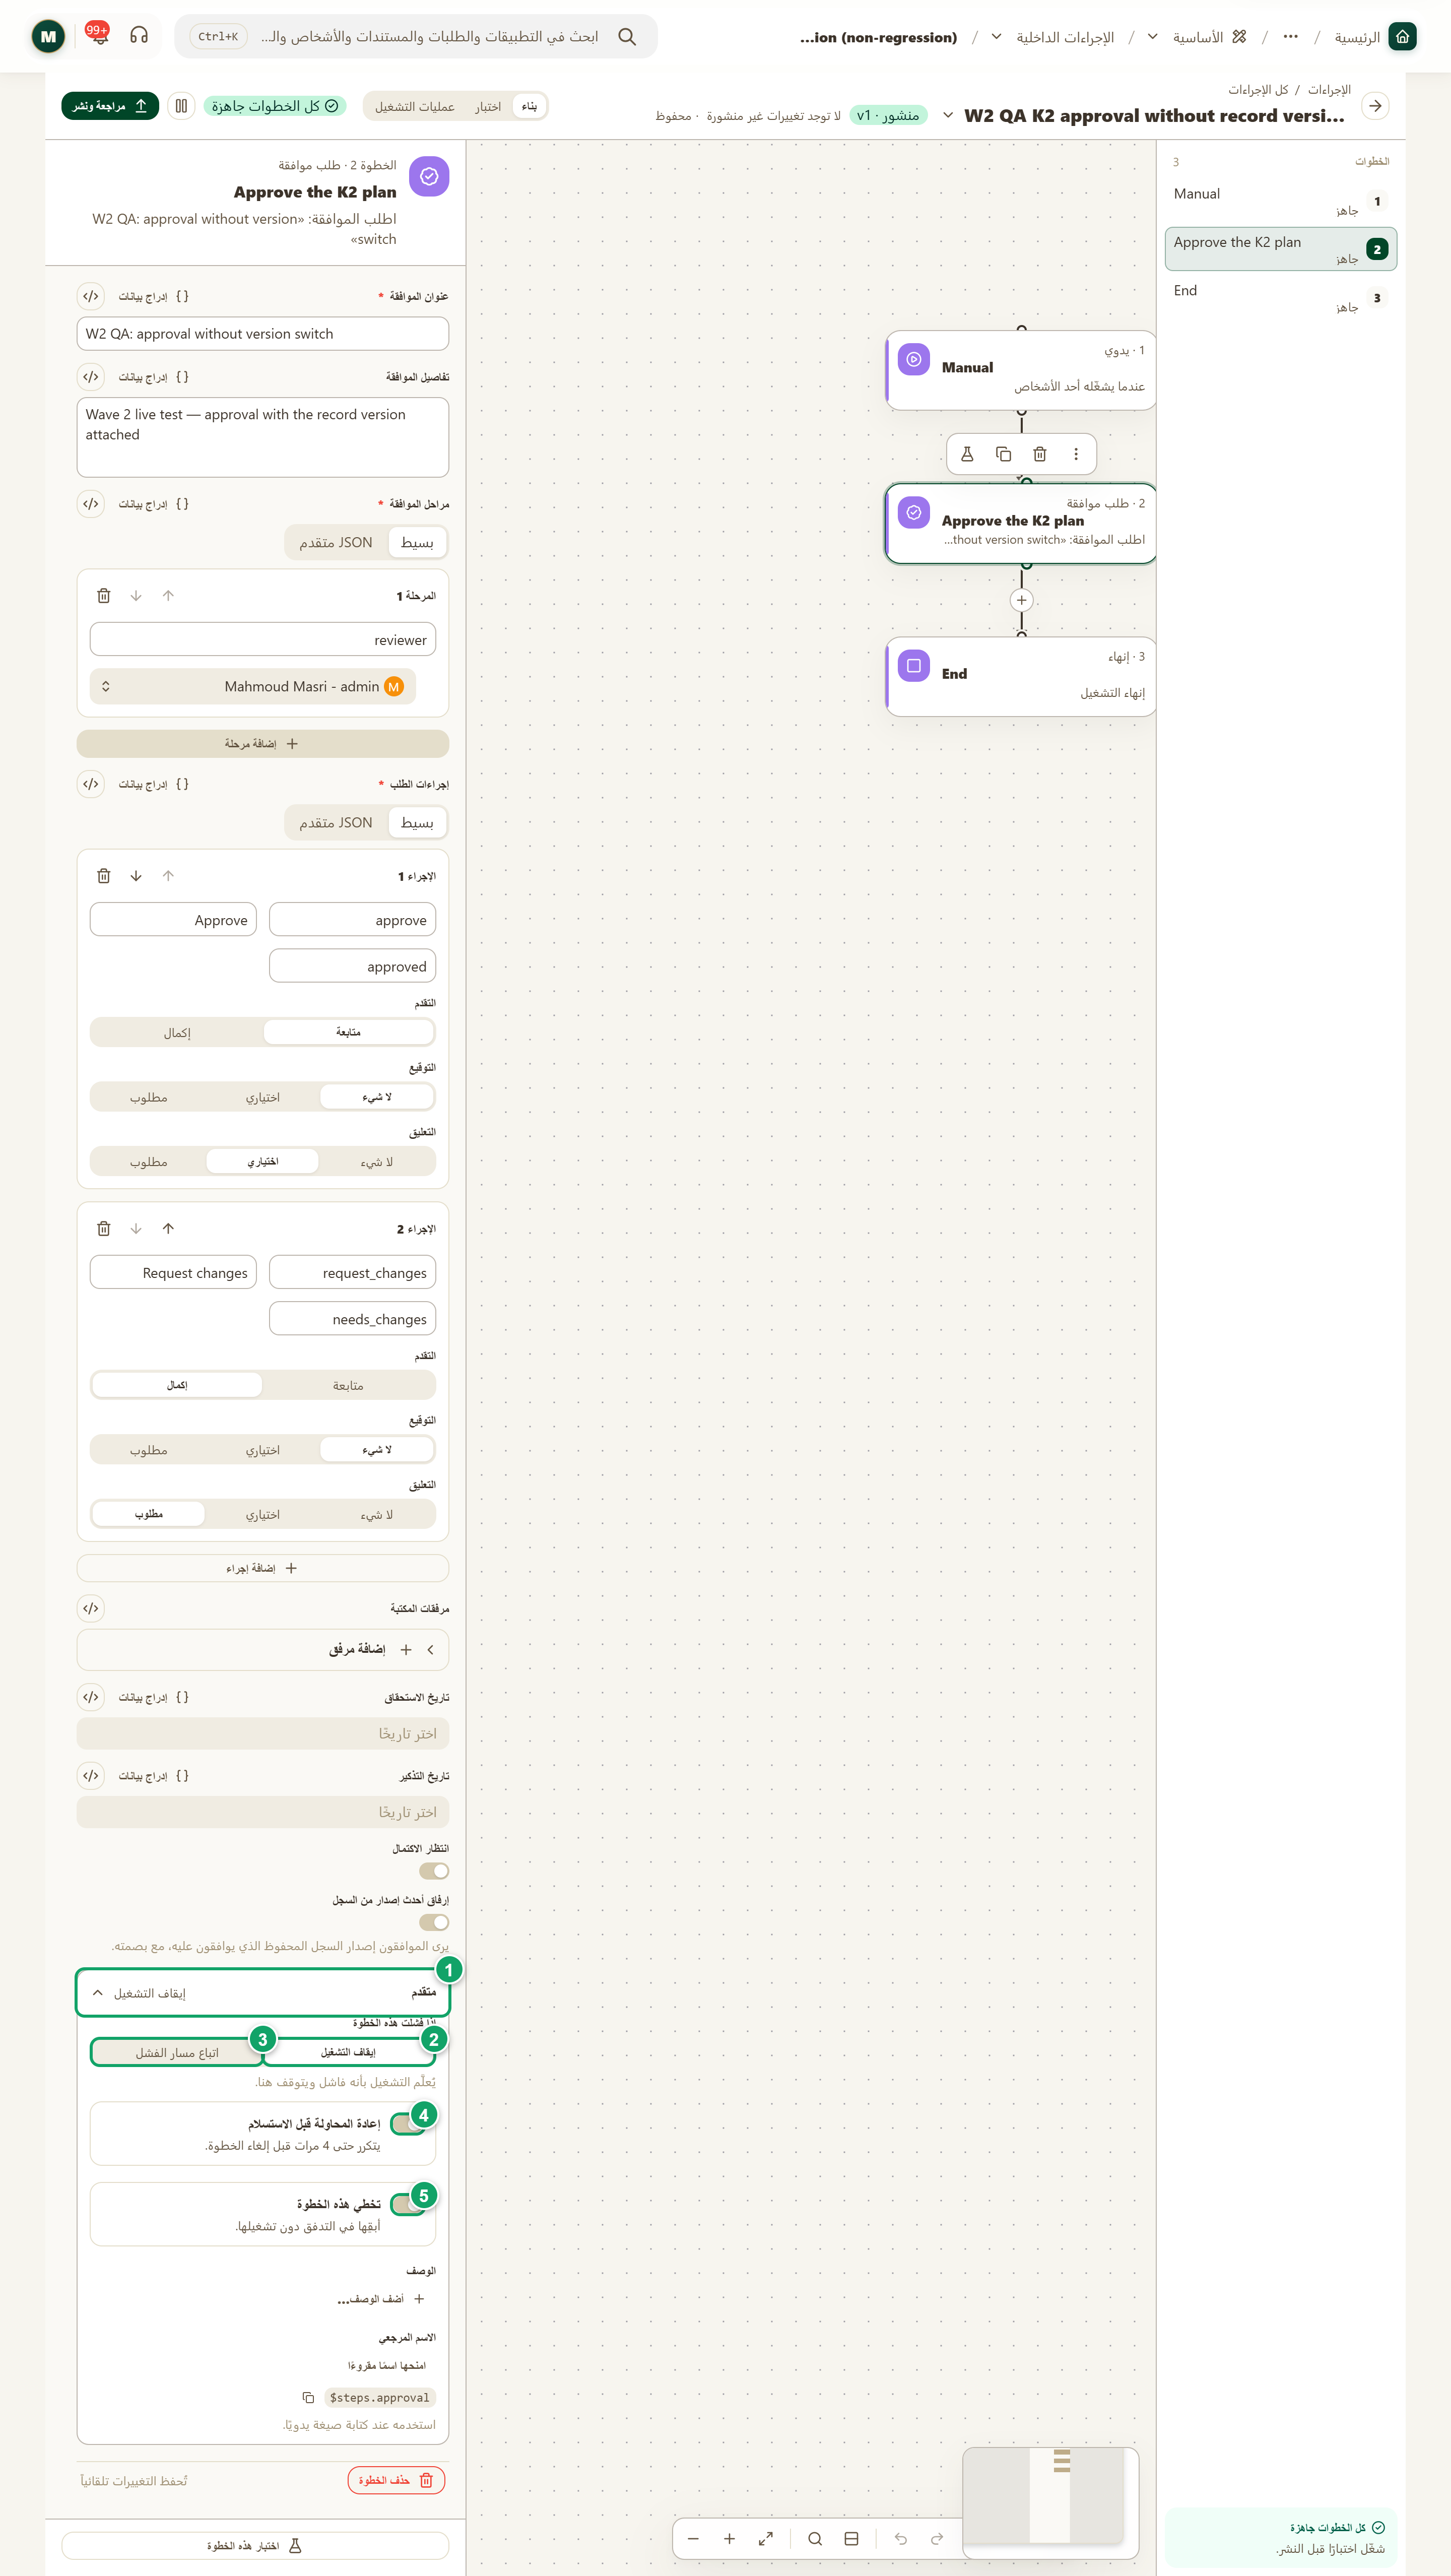
\includegraphics[width=0.95\linewidth,height=0.72\textheight,keepaspectratio]{figures/screens/ch06-isop-errors-ar.png}
\caption{خيارات الفشل والتخطي في «متقدم»}
\label{fig:builder-isop-errors-screen}
\shotnote{تعرض الصورة قسم «متقدم» مفتوحاً في خطوة «طلب موافقة»، والاختيار فيه على الوضع الافتراضي «إيقاف التشغيل» مع إيقاف المفتاحين. ويُلخَّص الاختيار بجانب عنوان «متقدم»، فتعرف سلوك الخطوة عند الفشل دون أن تفتح القسم. ① «متقدم»: يفتح الخيارات. ② «إيقاف التشغيل»: يتوقف التشغيل عند هذه الخطوة. ③ «اتباع مسار الفشل»: يضيف مساري نجاح وفشل. ④ «إعادة المحاولة قبل الاستسلام»: حتى أربع محاولات. ⑤ «تخطي هذه الخطوة»: تبقى الخطوة دون أن تعمل.}
\end{figure}

\begin{table}[H]
\centering
\caption{خيارات الفشل والتخطي}
\label{tab:builder-isop-errors-options}
\begin{tabularx}{\linewidth}{R{3.6cm} Y}
\rcHeaderRow
\thh{الخيار} & \thh{ما يحدث}\\
إيقاف التشغيل & هو الخيار الافتراضي: يُعلَّم التشغيل بأنه فاشل ويتوقف عند هذه الخطوة.\\
اتباع مسار الفشل & يضيف بعد الخطوة مسارين، نجاح وفشل، فيتابع التشغيل في مسار الفشل عند الخطأ بدلاً من التوقف. وعند إلغائه يبقى مسار النجاح وحده.\\
إعادة المحاولة قبل الاستسلام & يعيد تنفيذ الخطوة حتى أربع مرات قبل اعتبارها فاشلة.\\
تخطي هذه الخطوة & يُبقي الخطوة في المسار دون تشغيلها، وتظهر على اللوحة بشارة «تم التخطي». ولا يتوفر لخطوات التحكم مثل «تفرّع شرطي» و«لكل عنصر» و«إنهاء».\\
\end{tabularx}
\end{table}

\begin{figure}[H]
\centering
\begin{tikzpicture}[node distance=0.5cm]
\node[stepBox] (a) {\RL{تنفيذ الخطوة}};
\node[stepBox,below=of a] (b) {\RL{خطأ أثناء التنفيذ}};
\node[stepBox,below=of b] (c) {\RL{إعادة المحاولة إن فُعّلت}};
\node[stepBox,below=of c] (d) {\RL{إيقاف أو مسار الفشل}};
\node[stepBox,below=of d] (e) {\RL{مراجعة التشغيل}};
\draw[flowsTo] (a) -- (b);
\draw[flowsTo] (b) -- (c);
\draw[flowsTo] (c) -- (d);
\draw[flowsTo] (d) -- (e);
\end{tikzpicture}
\rclegend
\caption{ما يحدث عند فشل خطوة}
\label{fig:builder-isop-errors-flow}
\shotnote{يبيّن المخطط أن إعادة المحاولة تأتي أولاً، ولا يُطبَّق اختيار الإيقاف أو مسار الفشل إلا بعد أن تستنفد المحاولات. وفي الحالتين يبقى الخطأ مسجلاً في عملية التشغيل، فتراجعه لتعرف سببه.}
\end{figure}

\subsection{خطوات العمل والتحقق}
\begin{enumerate}
\item اضغط الخطوة، ثم افتح «متقدم».
\item في «إذا فشلت هذه الخطوة»، اختر «إيقاف التشغيل» أو «اتباع مسار الفشل».
\item إذا اخترت مسار الفشل، فأضف على مسار الفشل في اللوحة الخطوات التي تعالج الخطأ.
\item فعّل «إعادة المحاولة قبل الاستسلام» للخطوات التي تتصل بخدمات قد تتأخر.
\end{enumerate}

\textbf{تحقق ومعالجة المشكلة:} عند اختيار مسار الفشل يجب أن ترى خطين يخرجان من الخطوة، وأن يُلخَّص الاختيار بجانب «متقدم». وإذا نسيت خطوة على «تخطي هذه الخطوة» فلن تعمل في أي تشغيل، فابحث في اللوحة عن شارة «تم التخطي» قبل النشر.

\clearpage
\section{الاتصالات والمتغيرات}
\label{sec:builder-feature-isop-connections}

بعض الخطوات تتصل بخدمات خارج \en{KayanOS}، فتحتاج إلى حساب في تلك الخدمة. وتحفظ هذه الحسابات في تبويب «الاتصالات»، فتختار الخطوة الاتصال بدلاً من أن تحمل كلمة مرور. أما «المتغيرات» فقيم مشفرة تخص المؤسسة، مثل رمز وصول أو رقم ثابت، تستخدمها في تعبيرات أي إجراء دون أن تكتبها في كل خطوة.

\textbf{المسار ومن يستخدمه:} «الإجراءات الداخلية» ← «الاتصالات» أو «المتغيرات»، أو حقل «الاتصال» داخل خطوة من «التكاملات». يستخدمها من يبني الإجراءات ويدير حسابات المؤسسة.

\begin{rcnote}[مثال: شركة الأفق]
يضيف المسؤول متغيراً اسمه \en{HZN\_ALEPPO\_EMAIL} يحمل بريد فرع حلب، ثم يستخدمه في التعبيرات بدلاً من كتابة العنوان في كل خطوة. وعندما يتغير البريد، يغيّر قيمة المتغير مرة واحدة.
\end{rcnote}

\begin{figure}[H]
\centering
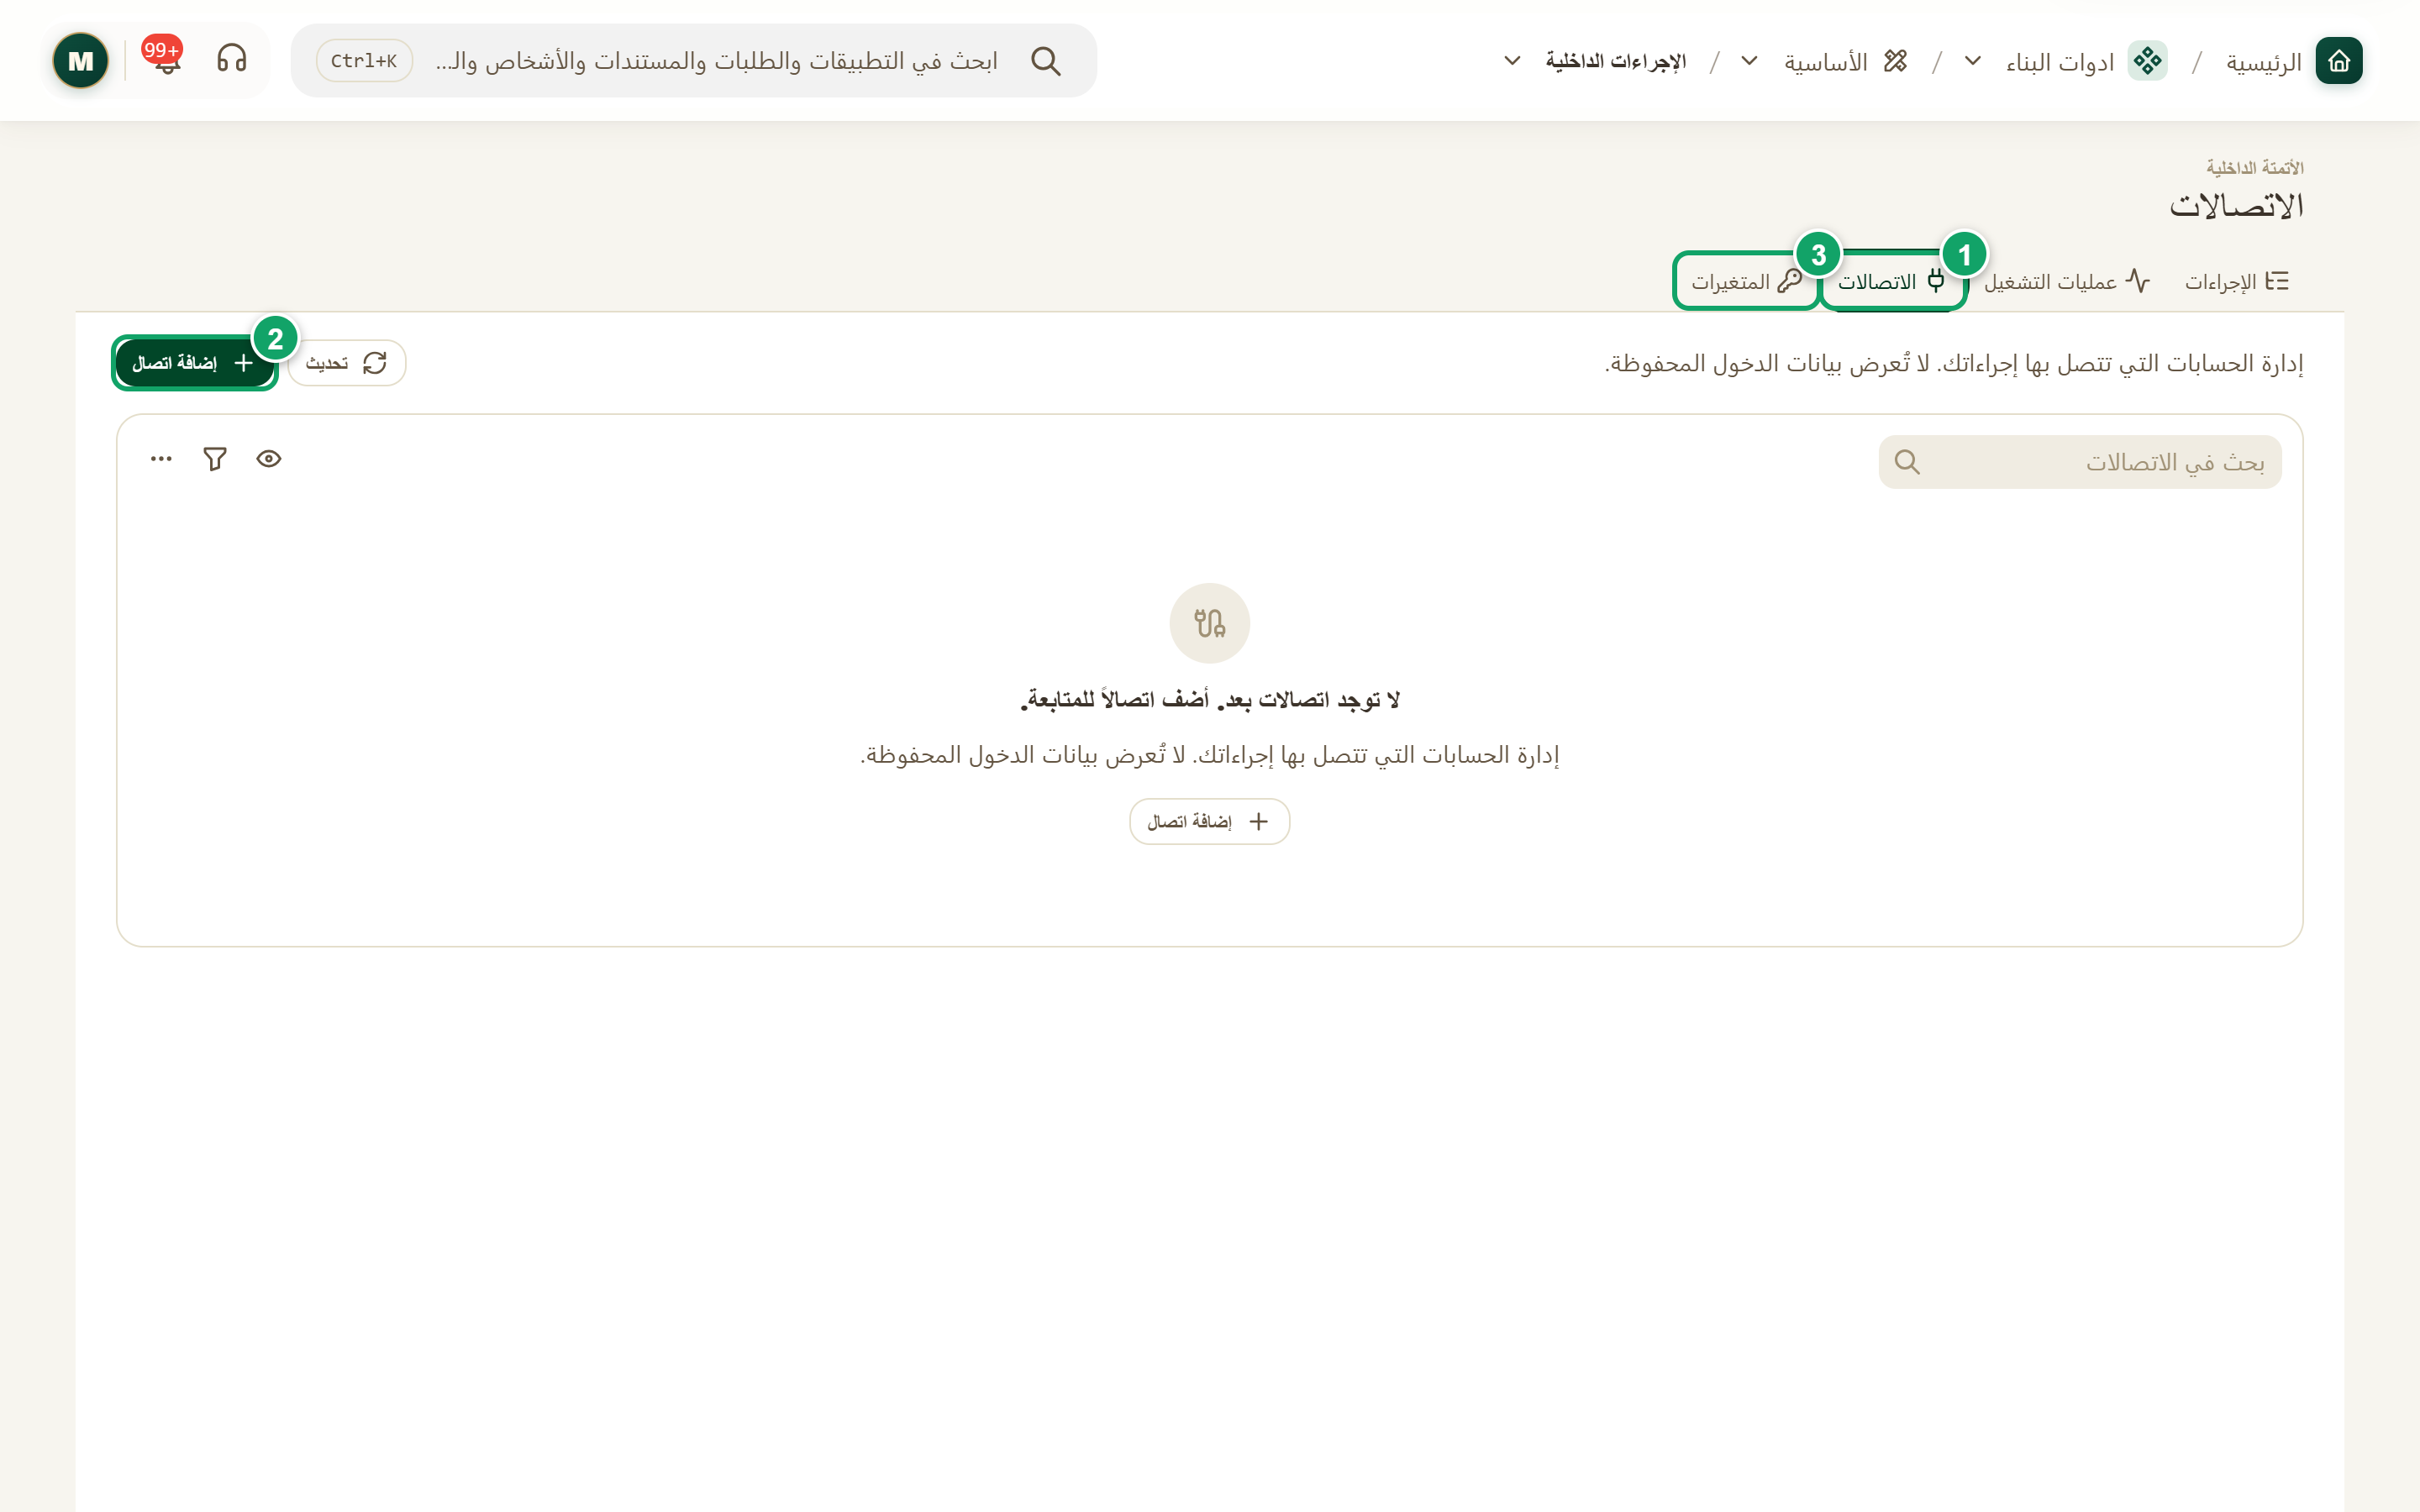
\includegraphics[width=0.95\linewidth,height=0.72\textheight,keepaspectratio]{figures/screens/ch06-isop-connections-ar.png}
\caption{تبويب «الاتصالات» في الإجراءات الداخلية}
\label{fig:builder-isop-connections-screen}
\shotnote{تعرض الصورة تبويب «الاتصالات» في مؤسسة الاختبار، وهو فارغ لأن أحداً لم يضف حساباً خارجياً بعد. وتوضح العبارة أعلى القائمة أن بيانات الدخول المحفوظة لا تُعرض أبداً، لذلك تختار الخطوة الاتصال باسمه فقط. ① «الاتصالات»: التبويب الذي يحفظ حسابات الخدمات الخارجية. ② «إضافة اتصال»: يبدأ ربط حساب جديد. ③ «المتغيرات»: التبويب المجاور للقيم المشفّرة التي تستخدمها التعبيرات.}
\end{figure}

\begin{table}[H]
\centering
\caption{إدارة الاتصالات}
\label{tab:builder-isop-connections-parts}
\begin{tabularx}{\linewidth}{R{3.6cm} Y}
\rcHeaderRow
\thh{الأداة} & \thh{ما تفعله}\\
إضافة اتصال & تختار «التطبيق» ثم «طريقة الاتصال»: «تسجيل الدخول إلى حساب» في نافذة جديدة، أو إدخال «مفتاح API أو رمز الوصول». ثم تكتب «اسم الاتصال» وتضغط «حفظ الاتصال».\\
الحالة & «نشط»، أو «يلزم إعادة الاتصال» عندما تنتهي صلاحية الدخول.\\
اختبار & يتحقق من الاتصال ويعرض «نجح اختبار الاتصال» أو «فشل اختبار الاتصال».\\
تحديث الاتصال & يعيد تسجيل الدخول أو يستبدل بيانات الدخول، دون أن يغيّر الخطوات التي تستخدمه.\\
إعادة تسمية، حذف & عند الحذف تحتاج الخطوات التي تستخدم الاتصال إلى بديل.\\
\end{tabularx}
\end{table}

\begin{table}[H]
\centering
\caption{إدارة المتغيرات}
\label{tab:builder-isop-connections-variables}
\begin{tabularx}{\linewidth}{R{3.6cm} Y}
\rcHeaderRow
\thh{الأداة} & \thh{ما تفعله}\\
متغير جديد & تكتب «الاسم» بأحرف وأرقام وشرطة سفلية فقط، ثم «القيمة»، ثم تضغط «إنشاء متغير». ولا تظهر القيمة مرة أخرى بعد حفظها.\\
نسخ المرجع & ينسخ صيغة الإشارة إلى المتغير لتلصقها في تعبير.\\
تغيير القيمة & يستبدل القيمة المحفوظة بقيمة جديدة.\\
حذف المتغير & يحذف المتغير، فتفشل التعبيرات التي تستخدمه.\\
\end{tabularx}
\end{table}

\begin{figure}[H]
\centering
\begin{tikzpicture}[node distance=0.5cm]
\node[stepBox] (a) {\RL{إضافة اتصال أو متغير}};
\node[stepBox,below=of a] (b) {\RL{اختباره أو نسخ مرجعه}};
\node[stepBox,below=of b] (c) {\RL{اختياره في الخطوة}};
\node[stepBox,below=of c] (d) {\RL{تحديثه عند التغيير}};
\draw[flowsTo] (a) -- (b);
\draw[flowsTo] (b) -- (c);
\draw[flowsTo] (c) -- (d);
\end{tikzpicture}
\rclegend
\caption{دورة حياة الاتصال والمتغير}
\label{fig:builder-isop-connections-flow}
\shotnote{يوضح المخطط أن الاتصال أو المتغير يُنشأ مرة واحدة ثم تستخدمه خطوات كثيرة. لذلك يكفي تحديثه في مكانه عند تغيّر كلمة المرور أو القيمة، دون فتح كل إجراء يعتمد عليه.}
\end{figure}

\subsection{خطوات العمل والتحقق}
\begin{enumerate}
\item افتح تبويب «الاتصالات»، واضغط «إضافة اتصال»، واختر «التطبيق».
\item اختر «طريقة الاتصال»، وسجّل الدخول أو أدخل المفتاح، ثم اكتب «اسم الاتصال» واضغط «حفظ الاتصال».
\item اضغط «اختبار» بجانب الاتصال، ثم اختره في حقل «الاتصال» داخل الخطوة.
\item لإضافة متغير، افتح «المتغيرات» واضغط «متغير جديد»، ثم اضغط «نسخ المرجع» لتستخدمه في تعبير.
\end{enumerate}

\textbf{تحقق ومعالجة المشكلة:} يجب أن يظهر الاتصال بحالة «نشط». فإذا ظهر «اسمح بالنوافذ المنبثقة لربط هذا الحساب»، فاسمح بالنوافذ المنبثقة للموقع ثم أعد المحاولة. وإذا أصبحت الحالة «يلزم إعادة الاتصال»، فاضغط «تحديث الاتصال» وسجّل الدخول من جديد.

\clearpage
\section{اختبار الإجراء}
\label{sec:builder-feature-isop-testing}

يجرّب الاختبار المسودة قبل نشرها، فترى نتيجة كل خطوة على اللوحة. ويوفر وضع «اختبار» طريقتين: «محاكاة (آمنة)» تشغّل المسودة دون إنشاء سجلات أو إرسال أي شيء، و«تشغيل فعلي» يشغّل الإصدار المنشور بآثار حقيقية. وتستطيع كذلك أن تختبر خطوة واحدة دون تشغيل المسار كله.

\textbf{المسار ومن يستخدمه:} المحرر ← «اختبار» ← لوحة «اختبار هذه المسودة»، أو لوحة الخطوة ← «اختبار هذه الخطوة». يستخدمه من يبني الإجراء قبل كل نشر.

\begin{rcnote}[مثال: شركة الأفق]
يكتب المسؤول في «بيانات الاختبار» طلب زيارة لفرع حلب، ثم يشغّل «محاكاة (آمنة)» (③). فيرى أن المسار وصل إلى «طلب موافقة» دون أن يصل أي طلب حقيقي إلى سارة الخطيب.
\end{rcnote}

\begin{figure}[H]
\centering
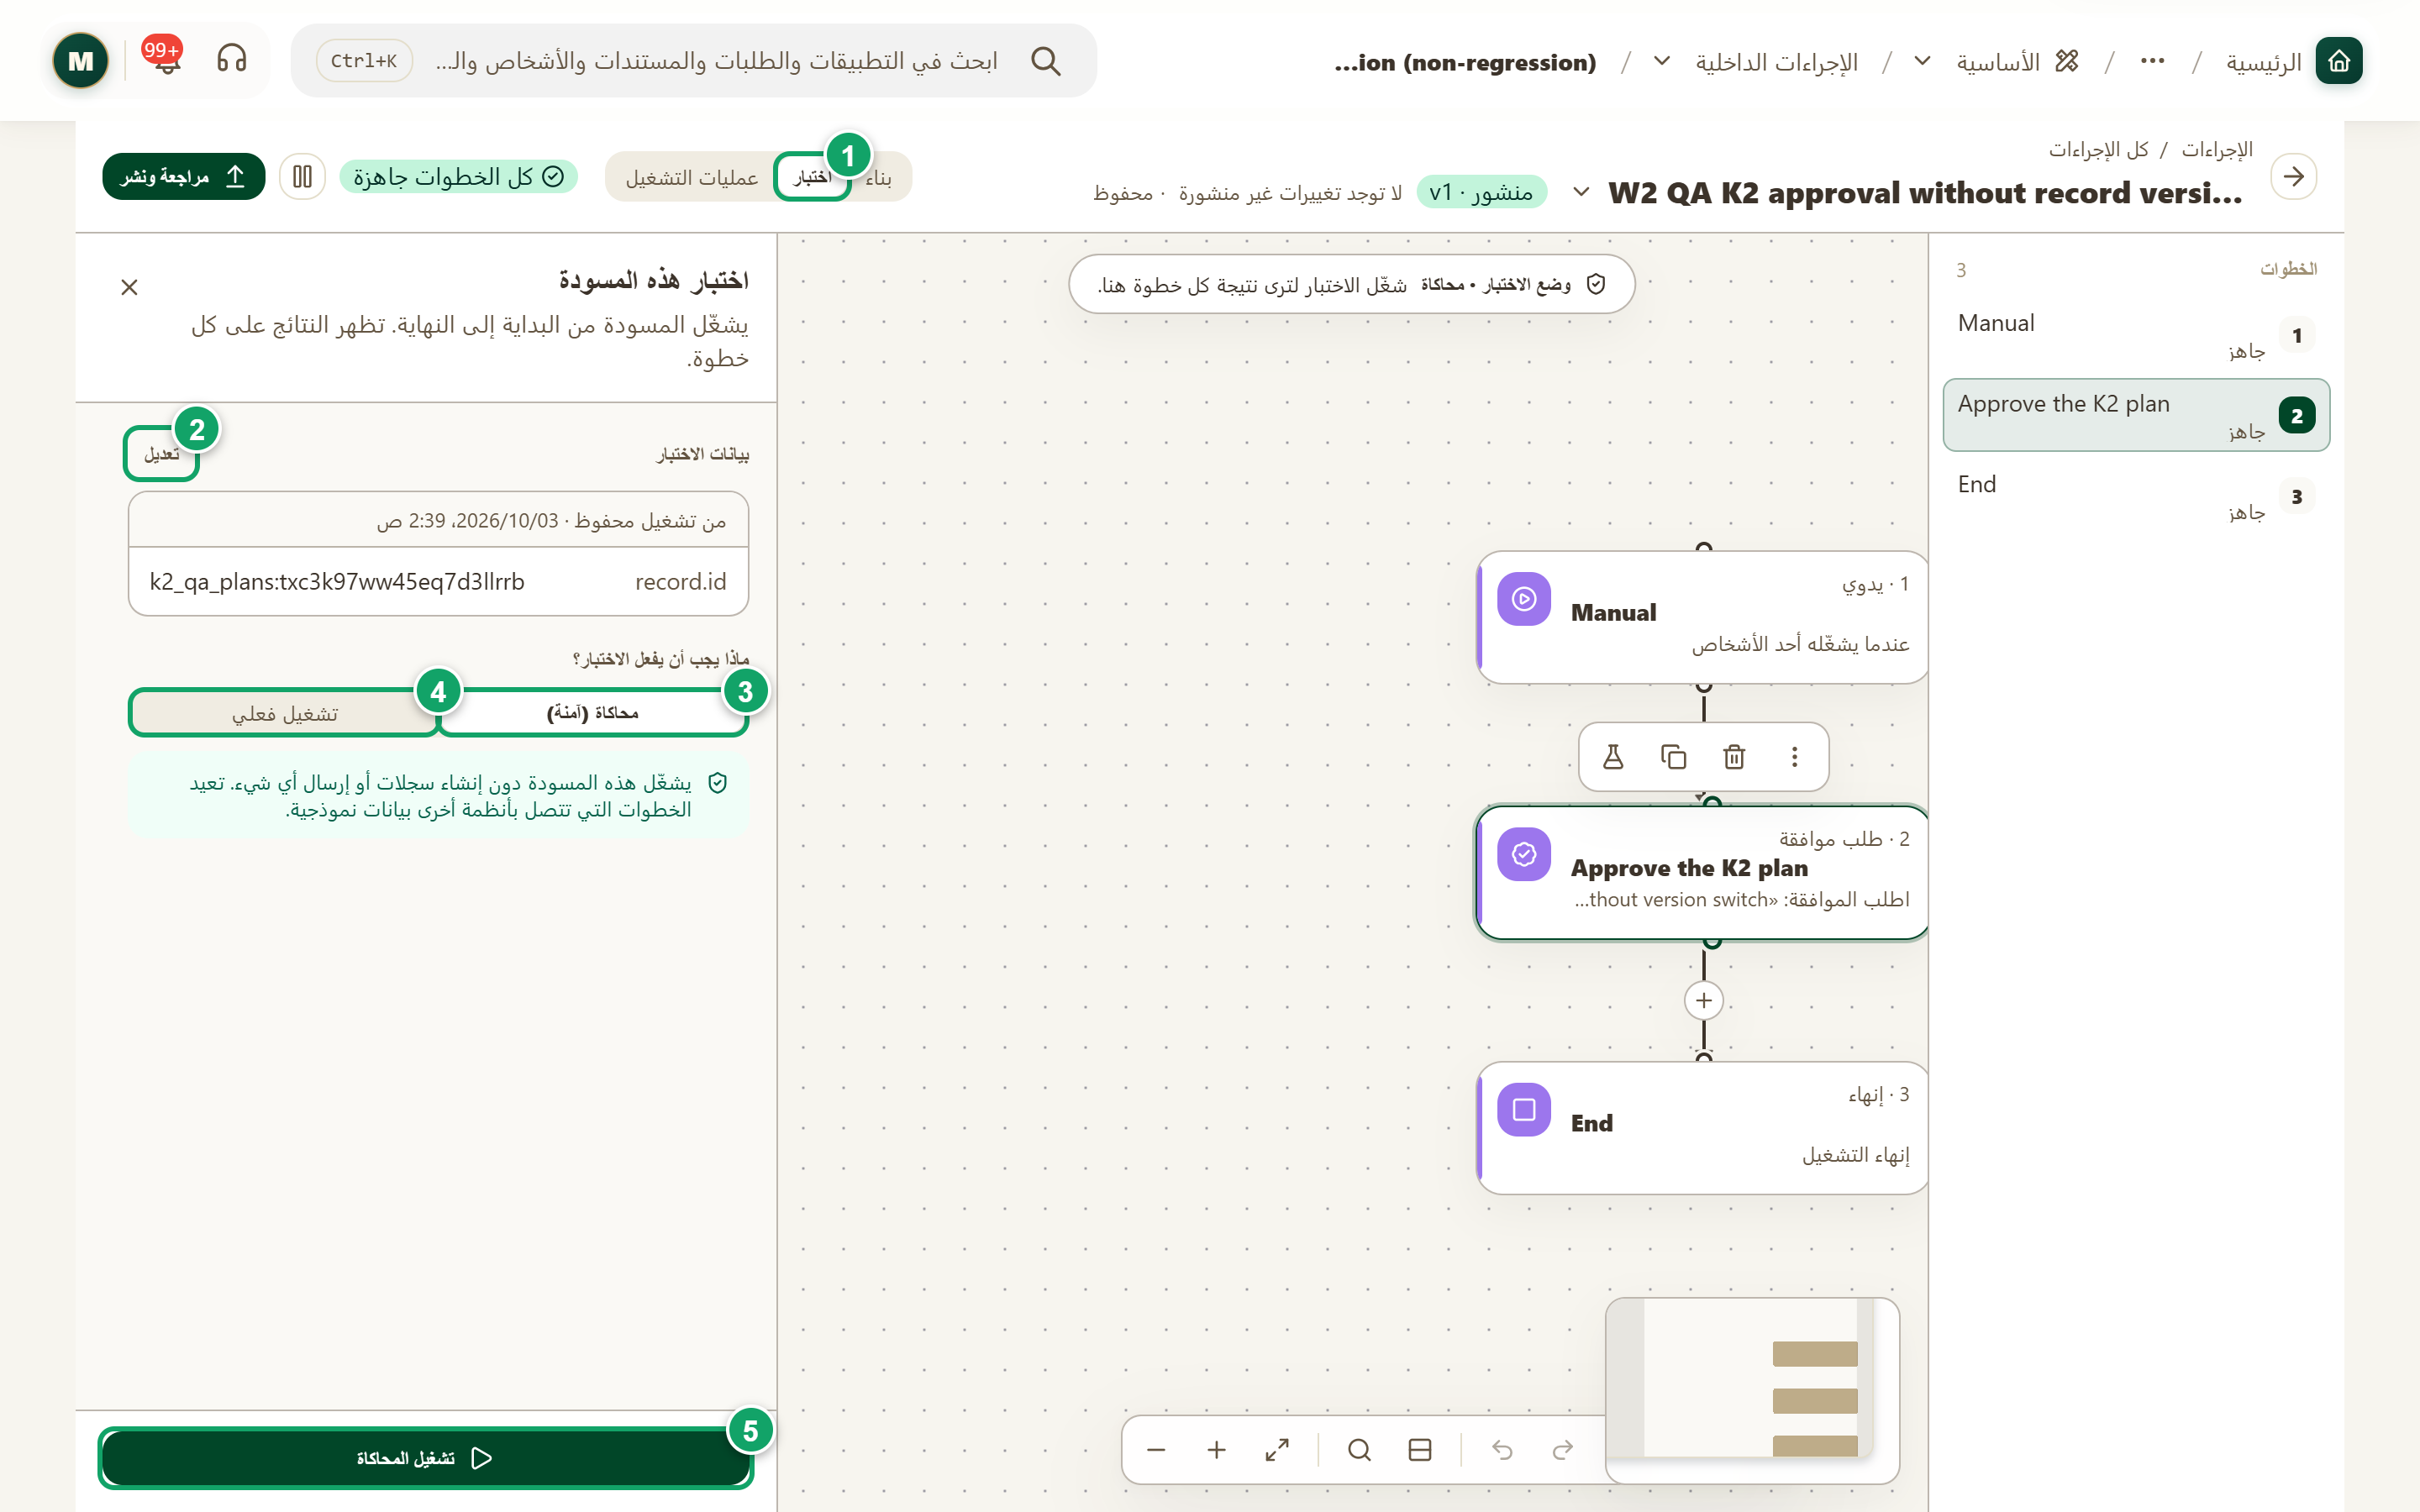
\includegraphics[width=0.95\linewidth,height=0.72\textheight,keepaspectratio]{figures/screens/ch06-isop-testing-ar.png}
\caption{لوحة «اختبار هذه المسودة» في وضع «اختبار»}
\label{fig:builder-isop-testing-screen}
\shotnote{تعرض الصورة الإجراء الاختباري في وضع «اختبار»، وبيانات الاختبار مأخوذة من تشغيل محفوظ، والاختيار على «محاكاة (آمنة)». ولم يُشغَّل أي اختبار عند الالتقاط، فاللوحة تبيّن ما تختاره قبل التشغيل لا نتيجته. ① «اختبار»: الوضع الذي تجرّب فيه المسودة. ② «تعديل»: يغيّر بيانات الاختبار. ③ «محاكاة (آمنة)»: تجربة بلا أثر حقيقي. ④ «تشغيل فعلي»: تشغيل للإصدار المنشور بآثار حقيقية. ⑤ «تشغيل المحاكاة»: يبدأ التجربة.}
\end{figure}

\begin{table}[H]
\centering
\caption{أجزاء لوحة الاختبار}
\label{tab:builder-isop-testing-panel}
\begin{tabularx}{\linewidth}{R{3.6cm} Y}
\rcHeaderRow
\thh{الجزء} & \thh{ما يقدمه}\\
بيانات الاختبار & البيانات التي يبدأ بها المشغّل. تعدّلها بـ«تعديل»، أو تختار «استخدام بيانات آخر تشغيل». ويجب أن تكون كائن \en{JSON}.\\
ماذا يجب أن يفعل الاختبار؟ & «محاكاة (آمنة)»: تشغّل المسودة، وتعيد الخطوات المتصلة بأنظمة أخرى بيانات نموذجية. «تشغيل فعلي»: يشغّل الإصدار المنشور، فتُنشأ السجلات وتُرسل الرسائل.\\
الموافقة على التشغيل الفعلي & مربع تؤكد فيه أن التشغيل قد يُحدث آثاراً فعلية وقد ينتظر استجابات خارجية. ولا يعمل الزر قبل تأكيده.\\
أحدث اختبار & «نجح الاختبار» أو «فشل الاختبار عند» خطوة محددة أو «الاختبار بانتظار رد»، مع عدد الخطوات والمدة و«السجلات والتفاصيل».\\
اختبار هذه الخطوة فقط & يشغّل الخطوة المختارة وحدها ببيانات اختبار محفوظة. ولخطوات \en{Kayan} ينفّذ إجراءً حقيقياً، فيطلب موافقتك قبل التشغيل.\\
\end{tabularx}
\end{table}

\begin{figure}[H]
\centering
\begin{tikzpicture}[node distance=0.5cm]
\node[stepBox] (a) {\RL{تجهيز بيانات الاختبار}};
\node[stepBox,below=of a] (b) {\RL{محاكاة آمنة للمسودة}};
\node[stepBox,below=of b] (c) {\RL{قراءة النتيجة على الخطوات}};
\node[stepBox,below=of c] (d) {\RL{إصلاح الخطوة وإعادة الاختبار}};
\node[stepBox,below=of d] (e) {\RL{تشغيل فعلي بعد النشر}};
\draw[flowsTo] (a) -- (b);
\draw[flowsTo] (b) -- (c);
\draw[flowsTo] (c) -- (d);
\draw[flowsTo] (d) -- (e);
\end{tikzpicture}
\rclegend
\caption{من المحاكاة إلى التشغيل الفعلي}
\label{fig:builder-isop-testing-flow}
\shotnote{يضع المخطط المحاكاة قبل كل شيء لأنها تختبر المسودة نفسها دون أي أثر على البيانات أو الأشخاص. أما التشغيل الفعلي فيأتي أخيراً، لأنه لا يعمل إلا على الإصدار المنشور وقد يُنشئ سجلات ويرسل طلبات حقيقية.}
\end{figure}

\subsection{خطوات العمل والتحقق}
\begin{enumerate}
\item اضغط «اختبار» في رأس المحرر، ثم اضغط «تعديل» في «بيانات الاختبار» واكتب القيم التي تريد تجربتها، واضغط «تم».
\item اختر «محاكاة (آمنة)»، ثم اضغط «تشغيل المحاكاة».
\item اقرأ النتيجة على كل خطوة، واضغط الخطوة الفاشلة لترى ما استلمته وما أعادته.
\item أصلح الخطوة في وضع «بناء»، ثم ارجع واضغط «تشغيل الاختبار مجددًا».
\item بعد النشر، إذا أردت تجربة فعلية، فاختر «تشغيل فعلي» وأكّد الموافقة، ثم اضغط زر التشغيل الفعلي.
\end{enumerate}

\textbf{تحقق ومعالجة المشكلة:} يجب أن يظهر «نجح الاختبار» في «أحدث اختبار». فإذا ظهر «خطوات ما زالت تحتاج إلى تهيئة»، فأكمل تلك الخطوات أولاً لأن الاختبار قد يتوقف عندها. وإذا لم يعمل «تشغيل فعلي»، فانشر الإجراء أولاً، وتأكد أن الخادم «متصل».

\clearpage
\section{عمليات التشغيل وسجلها}
\label{sec:builder-feature-isop-runs}

عملية التشغيل هي مرة واحدة عمل فيها الإجراء من المشغّل حتى النهاية أو حتى توقف. ويحفظ النظام لكل عملية حالتها ونتيجة كل خطوة فيها، فتعرف أين نجح الإجراء وأين فشل أو ينتظر. وتراجع العمليات من مكانين: وضع «عمليات التشغيل» في المحرر لإجراء واحد على لوحته، وتبويب «عمليات التشغيل» في الصفحة الرئيسية لكل الإجراءات معاً.

\textbf{المسار ومن يستخدمه:} المحرر ← «عمليات التشغيل»، أو «الإجراءات الداخلية» ← «عمليات التشغيل». يستخدمه من يبني الإجراء ومن يتابع تشغيله.

\begin{rcnote}[مثال: شركة الأفق]
يفتح المسؤول تشغيل الطلب \en{HZN-VR-0001} فيجده «بانتظار استجابة» عند «طلب موافقة»، مع مدة الانتظار ورابط يفتح الطلب. وبعد أن توافق سارة الخطيب يكتمل التشغيل وتظهر مهمة عمر حداد.
\end{rcnote}

\begin{figure}[H]
\centering
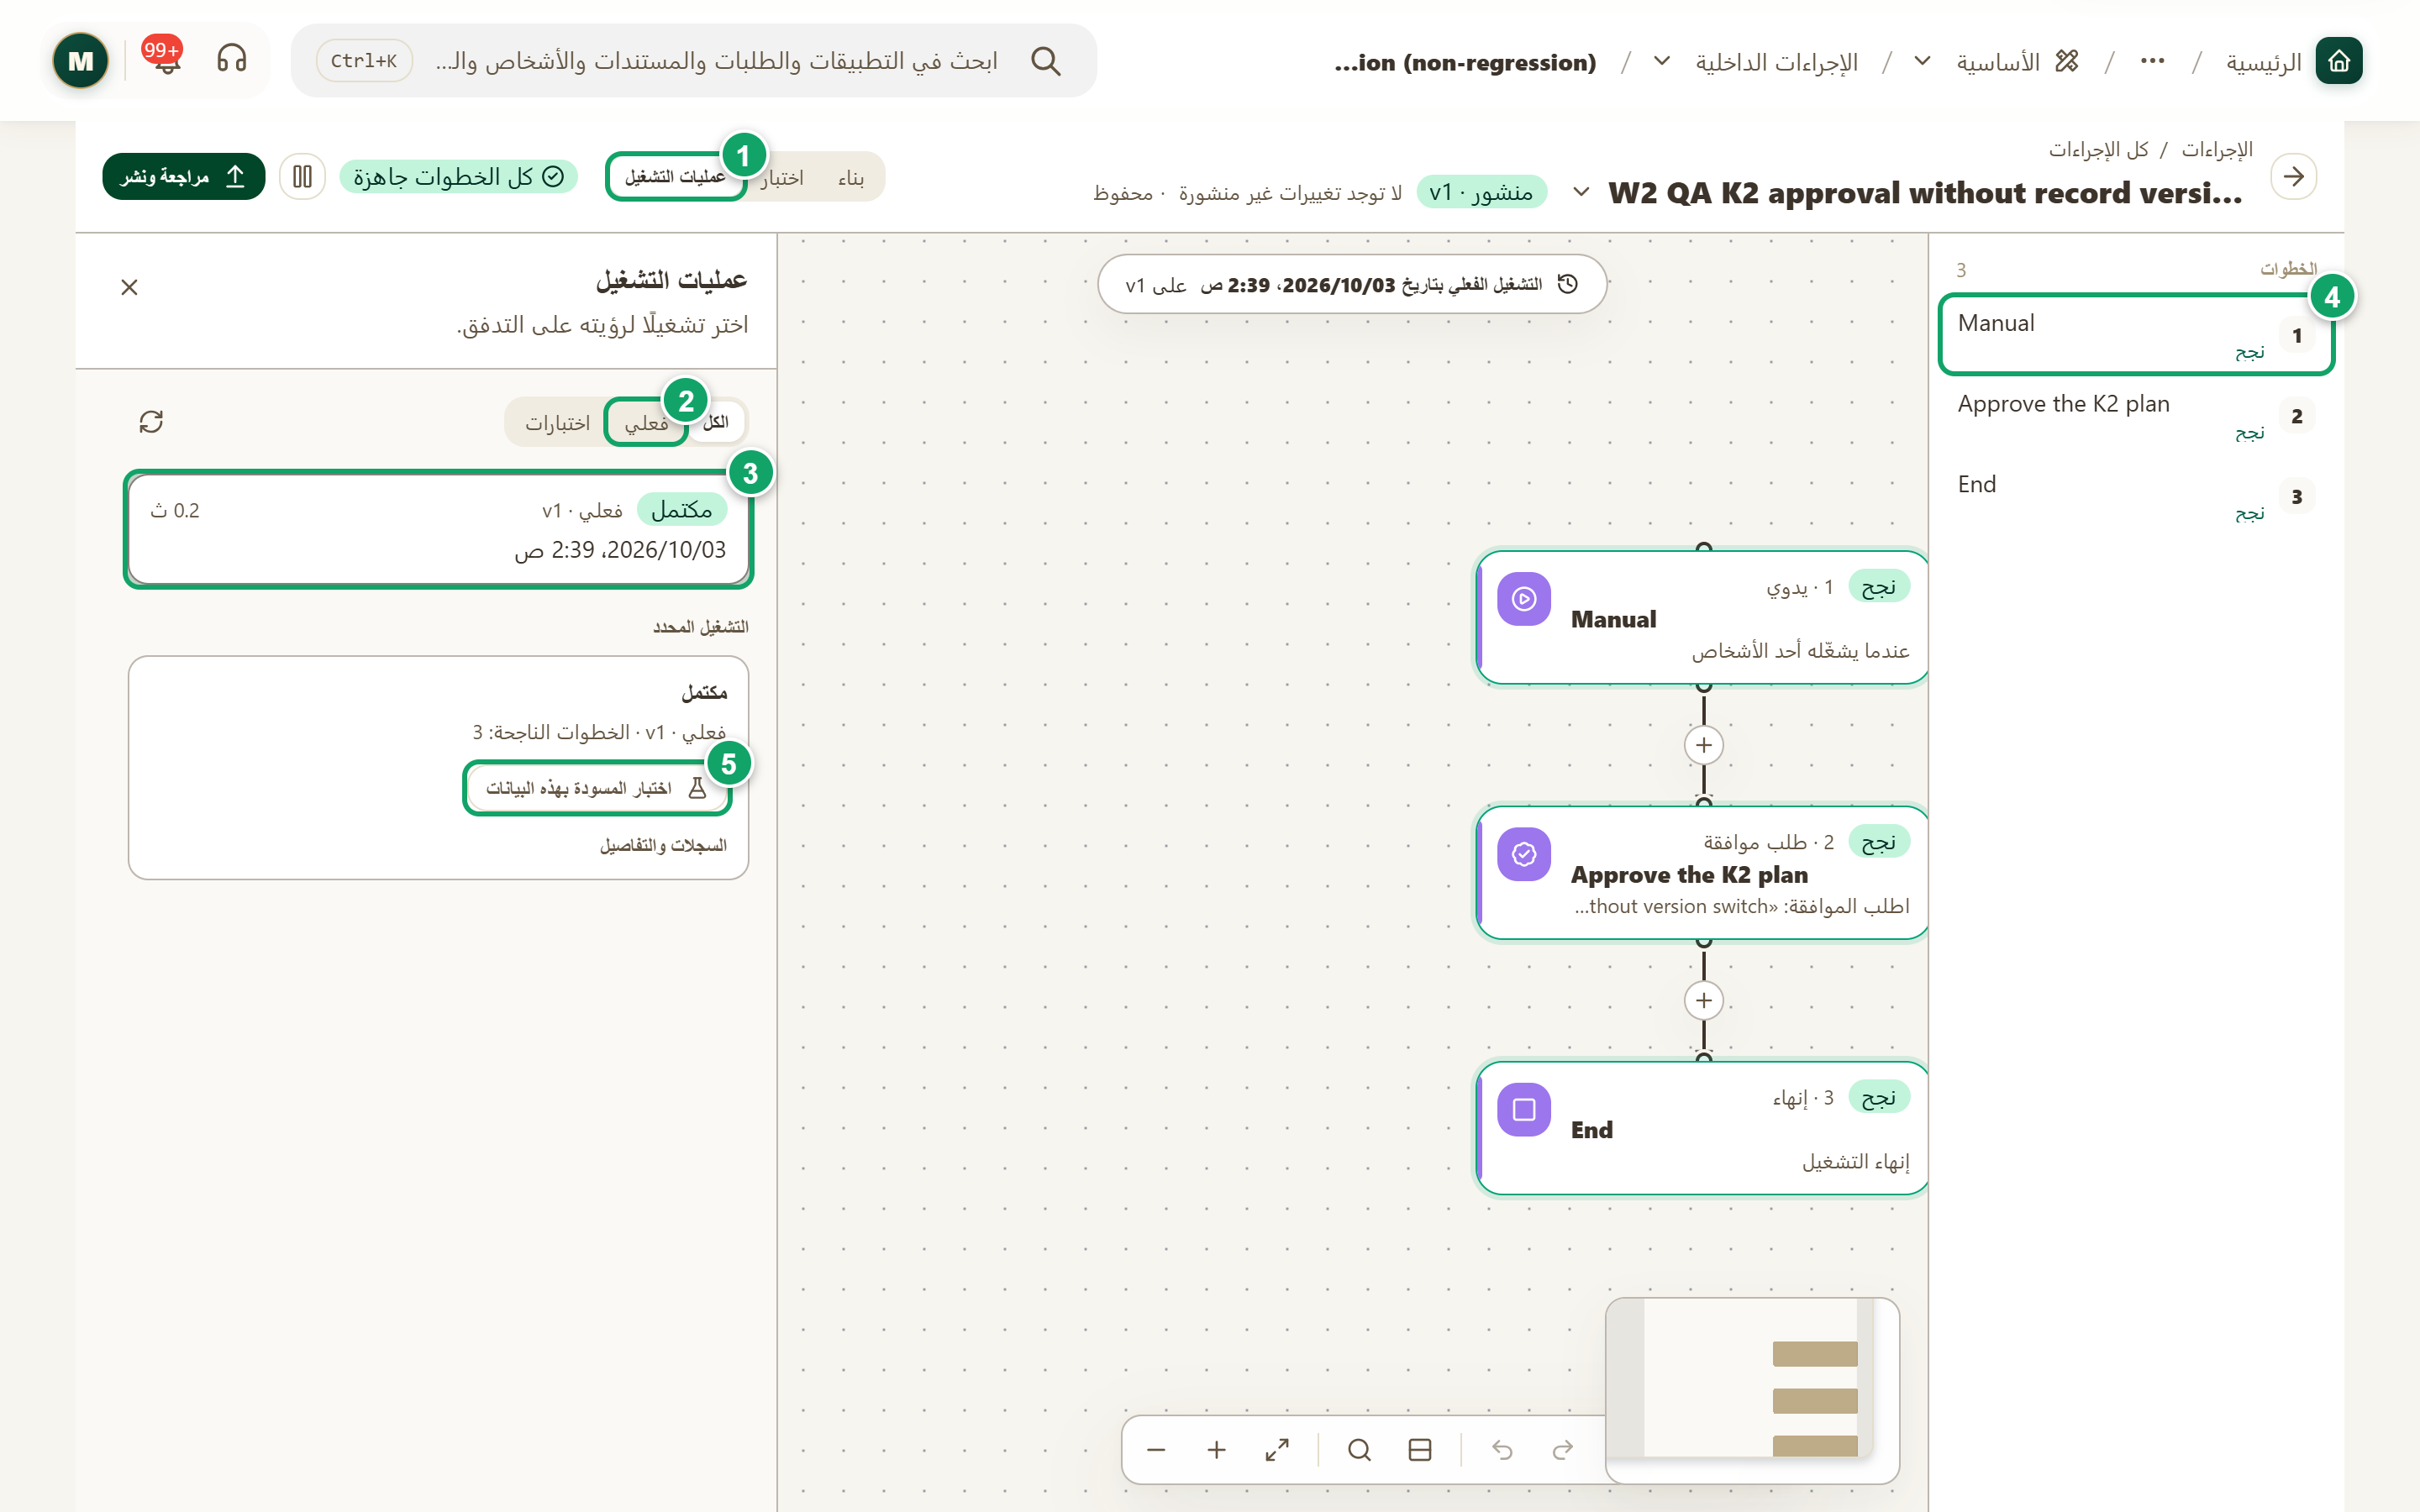
\includegraphics[width=0.95\linewidth,height=0.72\textheight,keepaspectratio]{figures/screens/ch06-isop-runs-ar.png}
\caption{تشغيل مكتمل معروض في وضع «عمليات التشغيل»}
\label{fig:builder-isop-runs-screen}
\shotnote{تعرض الصورة التشغيل الوحيد للإجراء الاختباري بعد اختياره، وقد ظهرت نتيجة كل خطوة على اللوحة وفي قائمة الخطوات. وبهذا ترى أين نجح التشغيل أو توقف دون أن تقرأ السجلات التقنية. ① «عمليات التشغيل»: الوضع الذي يعرض عمليات هذا الإجراء. ② «فعلي»: يُظهر العمليات الحقيقية دون الاختبارات. ③ بطاقة التشغيل «مكتمل»: تختارها لتراه على اللوحة. ④ «نجح»: نتيجة الخطوة في هذا التشغيل. ⑤ «اختبار المسودة بهذه البيانات»: يعيد تجربة المسودة ببيانات التشغيل نفسه.}
\end{figure}

\begin{table}[H]
\centering
\caption{حالات عملية التشغيل}
\label{tab:builder-isop-runs-statuses}
\begin{tabularx}{\linewidth}{R{3.6cm} Y}
\rcHeaderRow
\thh{الحالة} & \thh{معناها وما تفعله}\\
في قائمة الانتظار، قيد التشغيل & بدأت العملية ولم تنتهِ. ويمكنك إيقافها بـ«إلغاء التشغيل».\\
بانتظار استجابة & تنتظر موافقة أو نموذجاً أو توقيعاً أو مهمة أو حدثاً أو موعداً. وتعرض مدة الانتظار والموعد النهائي ورابطاً إلى الطلب أو السجل المرتبط.\\
مكتمل & وصلت العملية إلى نهايتها دون خطأ.\\
فشل & توقفت عند خطوة فاشلة. وتعرض الخطوة التي فشلت والخطأ، ويمكنك إعادتها بـ«إعادة تشغيل».\\
ملغي & أوقفها أحد قبل أن تنتهي.\\
\end{tabularx}
\end{table}

\begin{table}[H]
\centering
\caption{أين تراجع عمليات التشغيل؟}
\label{tab:builder-isop-runs-places}
\begin{tabularx}{\linewidth}{R{3.6cm} Y}
\rcHeaderRow
\thh{المكان} & \thh{ما يعرضه}\\
وضع «عمليات التشغيل» & عمليات هذا الإجراء مع تصفية «الكل» و«فعلي» و«اختبارات». وعند اختيار عملية تظهر نتيجة كل خطوة على اللوحة، مثل «نجح» و«فشل» و«بانتظار» و«تم تخطيه» و«لم يُبلَغ».\\
التشغيل المحدد & الإصدار والوضع وعدد الخطوات الناجحة، و«فشل عند» خطوة، و«فتح الخطوة» لقراءة مدخلاتها ومخرجاتها وخطئها، و«اختبار المسودة بهذه البيانات».\\
تبويب «عمليات التشغيل» & آخر خمسين عملية في كل الإجراءات، بأعمدة الإجراء والحالة والوضع ووقت البدء، مع بحث و«تحديث». والضغط على صف يفتح «تفاصيل التشغيل».\\
\end{tabularx}
\end{table}

\begin{figure}[H]
\centering
\begin{tikzpicture}[node distance=0.5cm]
\node[stepBox] (a) {\RL{وقوع الحدث}};
\node[stepBox,below=of a] (b) {\RL{في قائمة الانتظار}};
\node[stepBox,below=of b] (c) {\RL{قيد التشغيل}};
\node[stepBox,below=of c] (d) {\RL{بانتظار استجابة}};
\node[stepBox,below=of d] (e) {\RL{مكتمل أو فشل}};
\draw[flowsTo] (a) -- (b);
\draw[flowsTo] (b) -- (c);
\draw[flowsTo] (c) -- (d);
\draw[flowsTo] (d) -- (e);
\end{tikzpicture}
\rclegend
\caption{مراحل عملية التشغيل}
\label{fig:builder-isop-runs-flow}
\shotnote{يبيّن المخطط الطريق المعتاد لعملية فيها خطوة تنتظر شخصاً. فالانتظار مرحلة طبيعية وليس خطأً، وقد تستمر أياماً حتى يصل الرد أو تنتهي المهلة. أما العملية التي لا تنتظر أحداً فتنتقل من التشغيل إلى النهاية مباشرة.}
\end{figure}

\subsection{خطوات العمل والتحقق}
\begin{enumerate}
\item افتح الإجراء، واضغط «عمليات التشغيل»، واختر «فعلي» لترى العمليات الحقيقية فقط.
\item اختر عملية من القائمة، وراجع نتائج الخطوات على اللوحة.
\item إذا فشلت، فاضغط «فتح الخطوة» عند الخطوة الفاشلة واقرأ الخطأ.
\item أصلح السبب، ثم اضغط «إعادة تشغيل»، أو «اختبار المسودة بهذه البيانات» لتجرب الإصلاح أولاً.
\end{enumerate}

\textbf{تحقق ومعالجة المشكلة:} يجب أن تتغير حالة العملية بعد الإصلاح إلى «مكتمل». فإذا لم تجد أي عملية، فتأكد أن الإجراء منشور وغير متوقف، وأن الحدث وقع فعلاً بعد النشر. وإذا علقت عملية في الانتظار دون حاجة، فاضغط «إلغاء التشغيل».

\clearpage
\section{الرد على طلبات الموافقة}
\label{sec:builder-feature-isop-approvals}

عندما يصل الإجراء إلى خطوة «طلب موافقة»، يُنشئ طلباً يصل إلى المعتمدين، ثم ينتظر ردهم. ويرد المعتمد من صفحة «طلبات بانتظارك»، فيختار أحد إجراءات الطلب التي حددها من بنى الخطوة. وبعد الرد يتابع الإجراء مساره، ويستطيع إجراء آخر أن يبدأ عند الرد أو عند انتهاء الطلب.

\textbf{المسار ومن يستخدمه:} «طلبات بانتظارك» ← اضغط الطلب. يستخدمها المعتمدون، أما من بنى الإجراء فيتابع الطلب من التشغيل المنتظر.

\begin{rcnote}[مثال: شركة الأفق]
تفتح سارة الخطيب «طلبات بانتظارك» فتجد في «بانتظارك» (①) طلب «اعتماد زيارة فرع حلب»، فتضغط «موافقة» (③) وتوقّع. عندئذ يتابع الإجراء ويُنشئ مهمة تجهيز الزيارة لعمر حداد.
\end{rcnote}

\begin{figure}[H]
\centering
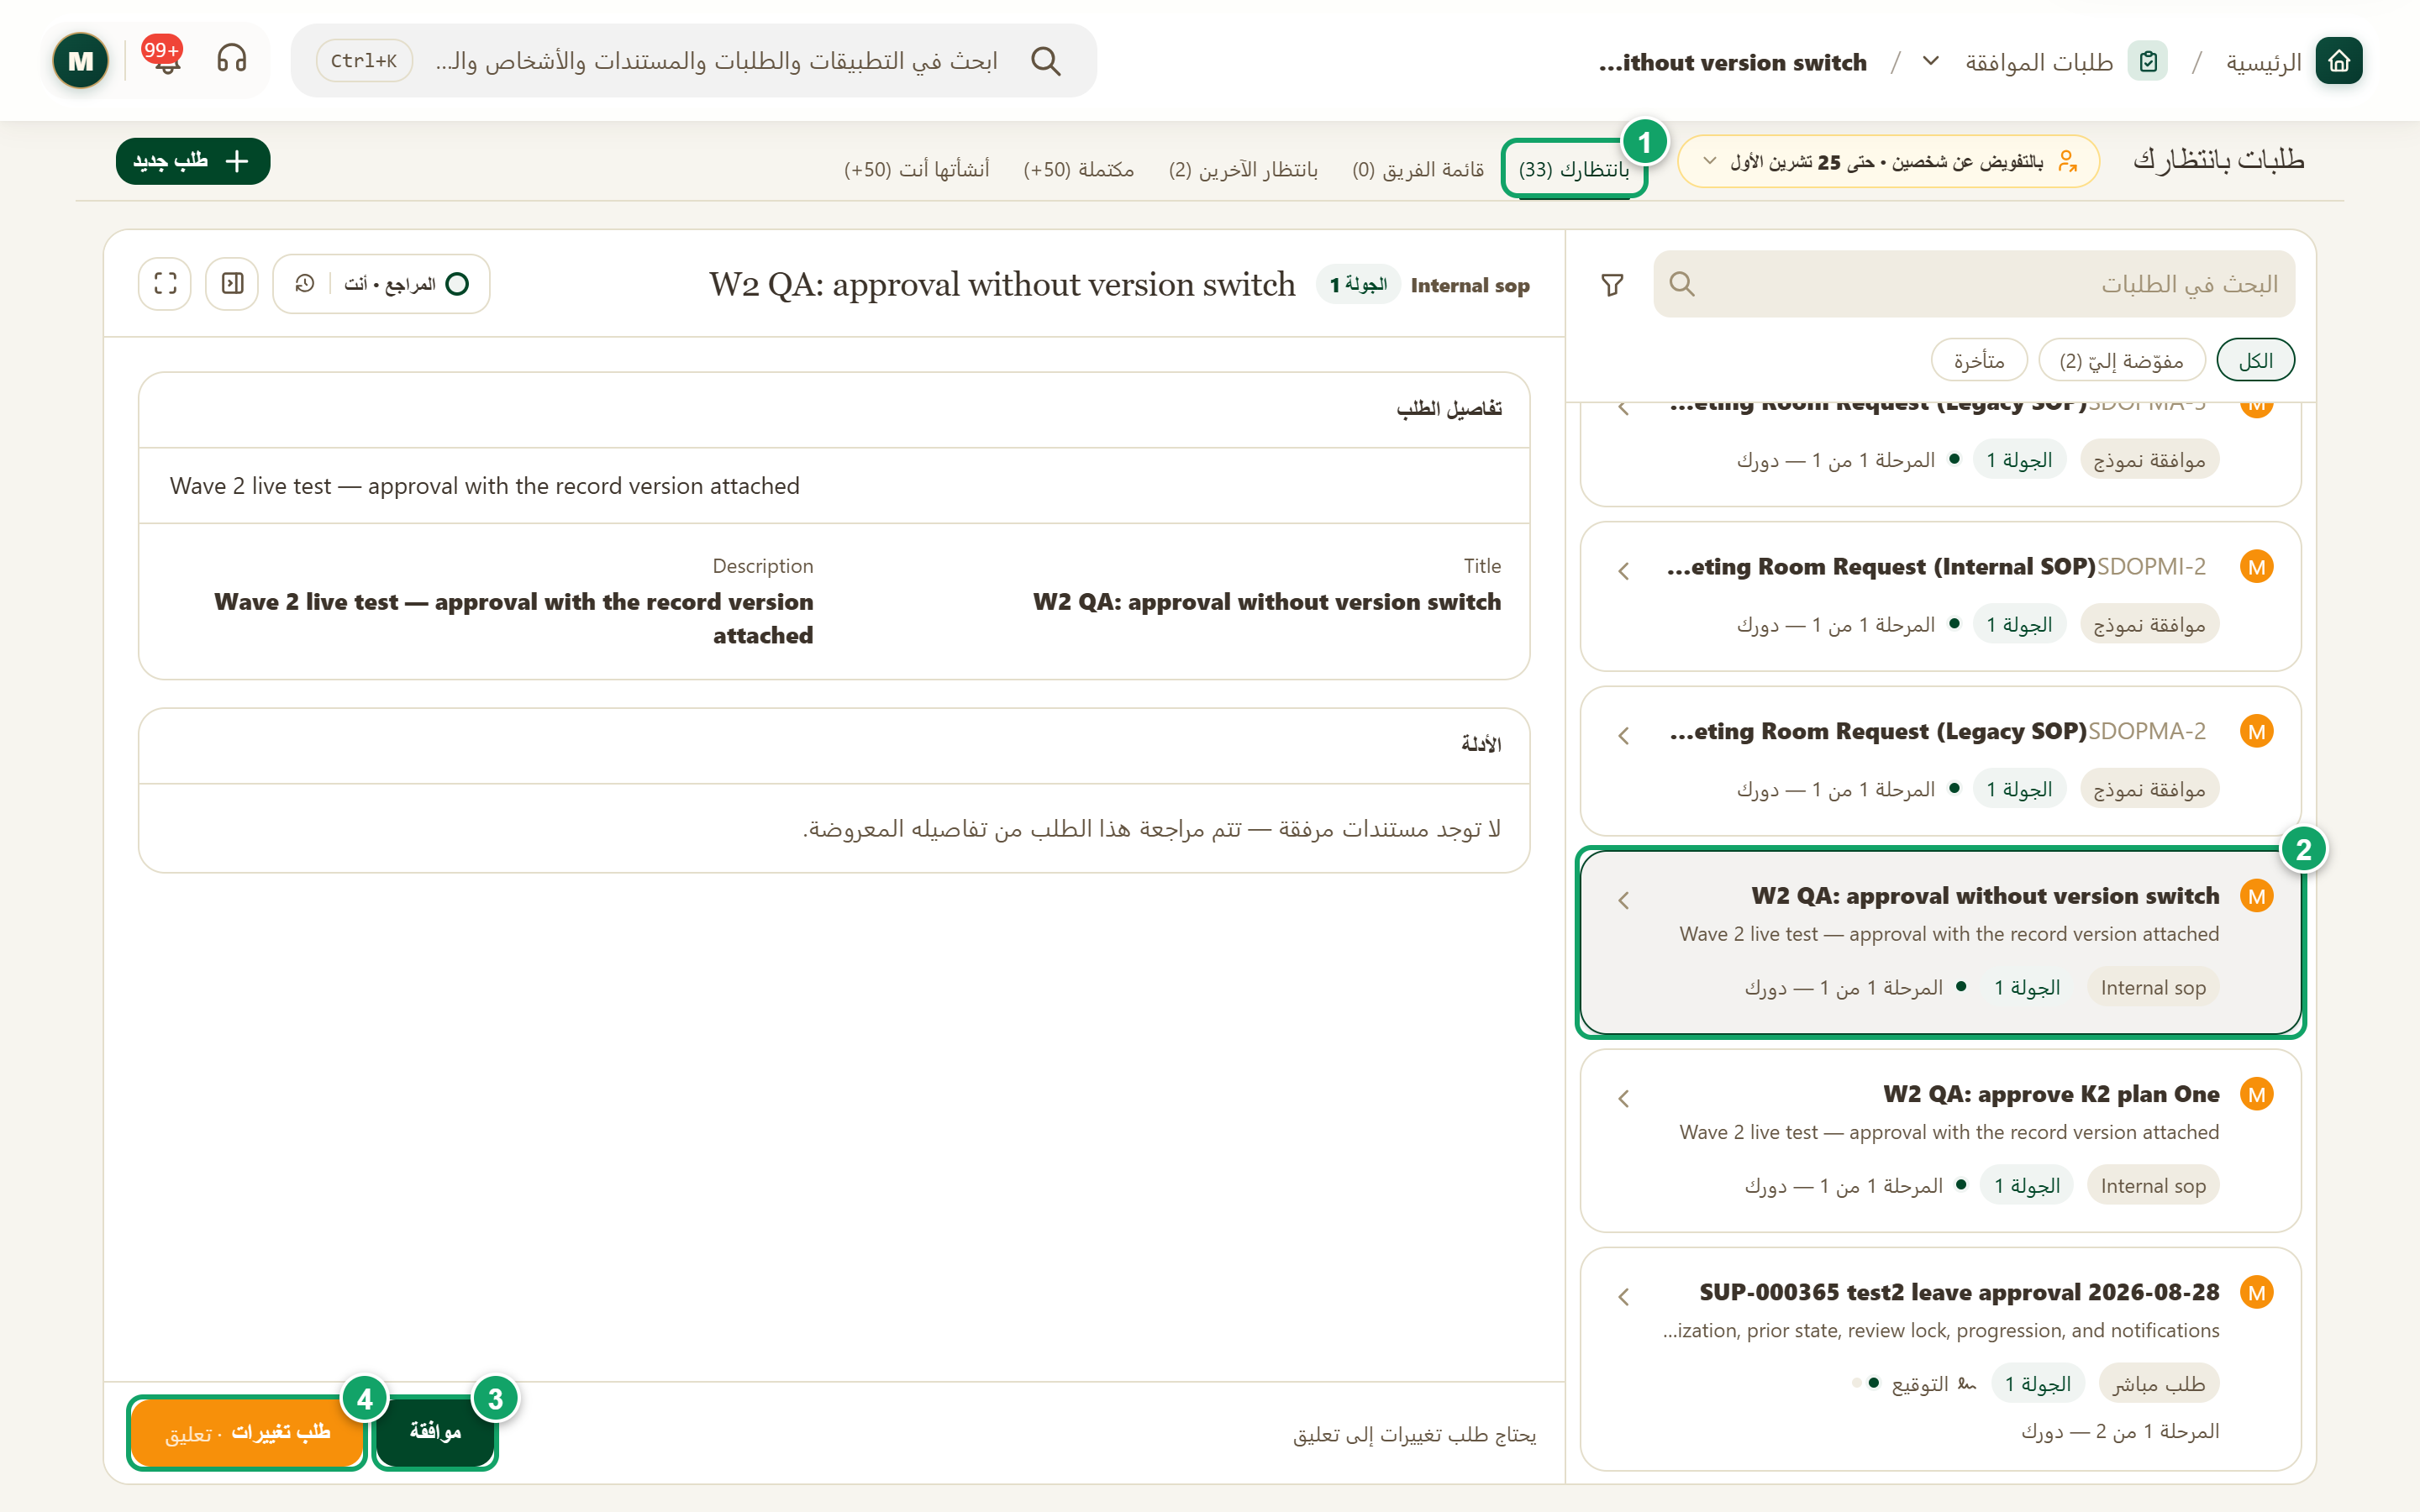
\includegraphics[width=0.95\linewidth,height=0.72\textheight,keepaspectratio]{figures/screens/ch06-isop-approvals-ar.png}
\caption{طلب موافقة من إجراء داخلي في «طلبات بانتظارك»}
\label{fig:builder-isop-approvals-screen}
\shotnote{تعرض الصورة صفحة «طلبات بانتظارك» في مؤسسة الاختبار، وقد اختير طلب أنشأته خطوة «طلب موافقة» من الإجراء الاختباري. وتظهر أزرار الرد بأسماء إجراءات الطلب التي حددها من بنى الخطوة، لذلك قد تختلف من إجراء إلى آخر. ① «بانتظارك»: التبويب الذي يجمع الطلبات المنتظرة لردك. ② بطاقة الطلب: تختارها لترى تفاصيله. ③ «موافقة»: إجراء الموافقة. ④ «طلب تغييرات»: إجراء يتطلب كتابة تعليق.}
\end{figure}

\begin{table}[H]
\centering
\caption{ما يحدث عند كل رد}
\label{tab:builder-isop-approvals-responses}
\begin{tabularx}{\linewidth}{R{3.6cm} Y}
\rcHeaderRow
\thh{الرد أو الحدث} & \thh{النتيجة}\\
الموافقة & الإجراء الجاهز في الخطوة، ويطلب توقيعاً ويكون التعليق اختيارياً. ويتابع الطلب إلى المرحلة التالية إن وُجدت.\\
طلب التغييرات & الإجراء الجاهز الثاني، والتعليق فيه إلزامي، وينهي الطلب بنتيجة طلب التغييرات.\\
انتهاء المهلة & إذا لم يصل رد خلال «المهلة الزمنية» انتهى الانتظار.\\
عند استجابة موافقة & مشغّل يبدأ إجراءً آخر مع كل رد على الطلب.\\
عند انتهاء موافقة & مشغّل يبدأ إجراءً آخر عندما يكتمل الطلب أو يُلغى أو تنتهي مهلته.\\
\end{tabularx}
\end{table}

\subsection{صفحة موافقات الإجراءات القديمة}

تبقى للإجراءات القديمة صفحة رد مستقلة يفتحها رابط الموافقة. وتعرض العنوان والتفاصيل وسياسة الموافقة وتاريخ الاستحقاق، وفيها «التعليق (اختياري)» بخمسمئة حرف على الأكثر، وزرّا «موافقة» و«رفض». ويُقبل رد واحد فقط، وتظهر حالة الطلب: «قيد الانتظار» أو «تمت الموافقة» أو «مرفوض» أو «منتهي الصلاحية» أو «ملغى».

\begin{figure}[H]
\centering
\begin{tikzpicture}[node distance=0.5cm]
\node[stepBox] (a) {\RL{خطوة طلب موافقة}};
\node[stepBox,below=of a] (b) {\RL{الطلب في طلبات بانتظارك}};
\node[stepBox,below=of b] (c) {\RL{رد المعتمد}};
\node[stepBox,below=of c] (d) {\RL{تسجيل النتيجة}};
\node[stepBox,below=of d] (e) {\RL{متابعة الإجراء}};
\draw[flowsTo] (a) -- (b);
\draw[flowsTo] (b) -- (c);
\draw[flowsTo] (c) -- (d);
\draw[flowsTo] (d) -- (e);
\end{tikzpicture}
\rclegend
\caption{رحلة طلب الموافقة}
\label{fig:builder-isop-approvals-flow}
\shotnote{يوضح المخطط أن الإجراء لا يقرر نيابةً عن المعتمد، بل يرسل الطلب وينتظر. فالنتيجة التي يسجلها الرد هي ما تقرؤه الخطوات التالية لتختار مسارها.}
\end{figure}

\subsection{خطوات العمل والتحقق}
\begin{enumerate}
\item افتح «طلبات بانتظارك»، واختر الطلب من تبويب «بانتظارك».
\item اقرأ عنوان الطلب وتفاصيله والسجل المرفق إن وُجد.
\item اضغط «موافقة» ووقّع، أو اضغط «طلب تغييرات» واكتب التعليق.
\item بصفتك من بنى الإجراء، افتح التشغيل في «عمليات التشغيل» وتحقق أنه تابع بعد الرد.
\end{enumerate}

\textbf{تحقق ومعالجة المشكلة:} يجب أن يخرج الطلب من «بانتظارك» ويظهر في «مكتملة»، وأن يتابع التشغيل بعد الرد. فإذا لم يجد المعتمد الطلب، فتأكد أنه في مراحل الموافقة، وأن التشغيل وصل فعلاً إلى خطوة «طلب موافقة». وإذا تأخر الرد، فأرسل تذكيراً من الطلب.

\clearpage
\section{المراجعة والنشر وسجل الإصدارات}
\label{sec:builder-feature-isop-publish}

لا يعمل الإجراء إلا بعد نشره، ولا تصل تعديلاتك إلى الإصدار المنشور حتى تنشرها من جديد. ويعرض «مراجعة ونشر» قبل النشر ما يجب إصلاحه، والتغييرات منذ الإصدار المنشور، ونتيجة آخر اختبار. وبعد النشر يُقفل الإصدار، فتكمل العمليات الجارية على إصدارها القديم، وتستخدم العمليات الجديدة الإصدار الجديد.

\textbf{المسار ومن يستخدمه:} المحرر ← «مراجعة ونشر»، وسجل الإصدارات من اسم الإجراء في رأس المحرر. يستخدمه من يبني الإجراء.

\begin{rcnote}[مثال: شركة الأفق]
يضيف المسؤول خطوة «إرسال إشعار» إلى الإجراء المنشور، فتظهر في «التغييرات منذ \en{v1} (المنشور)» بعلامة «مُضاف». فينشر \en{v2}، ويبقى طلب زيارة كان ينتظر موافقة سارة على \en{v1} حتى ينتهي.
\end{rcnote}

\begin{figure}[H]
\centering
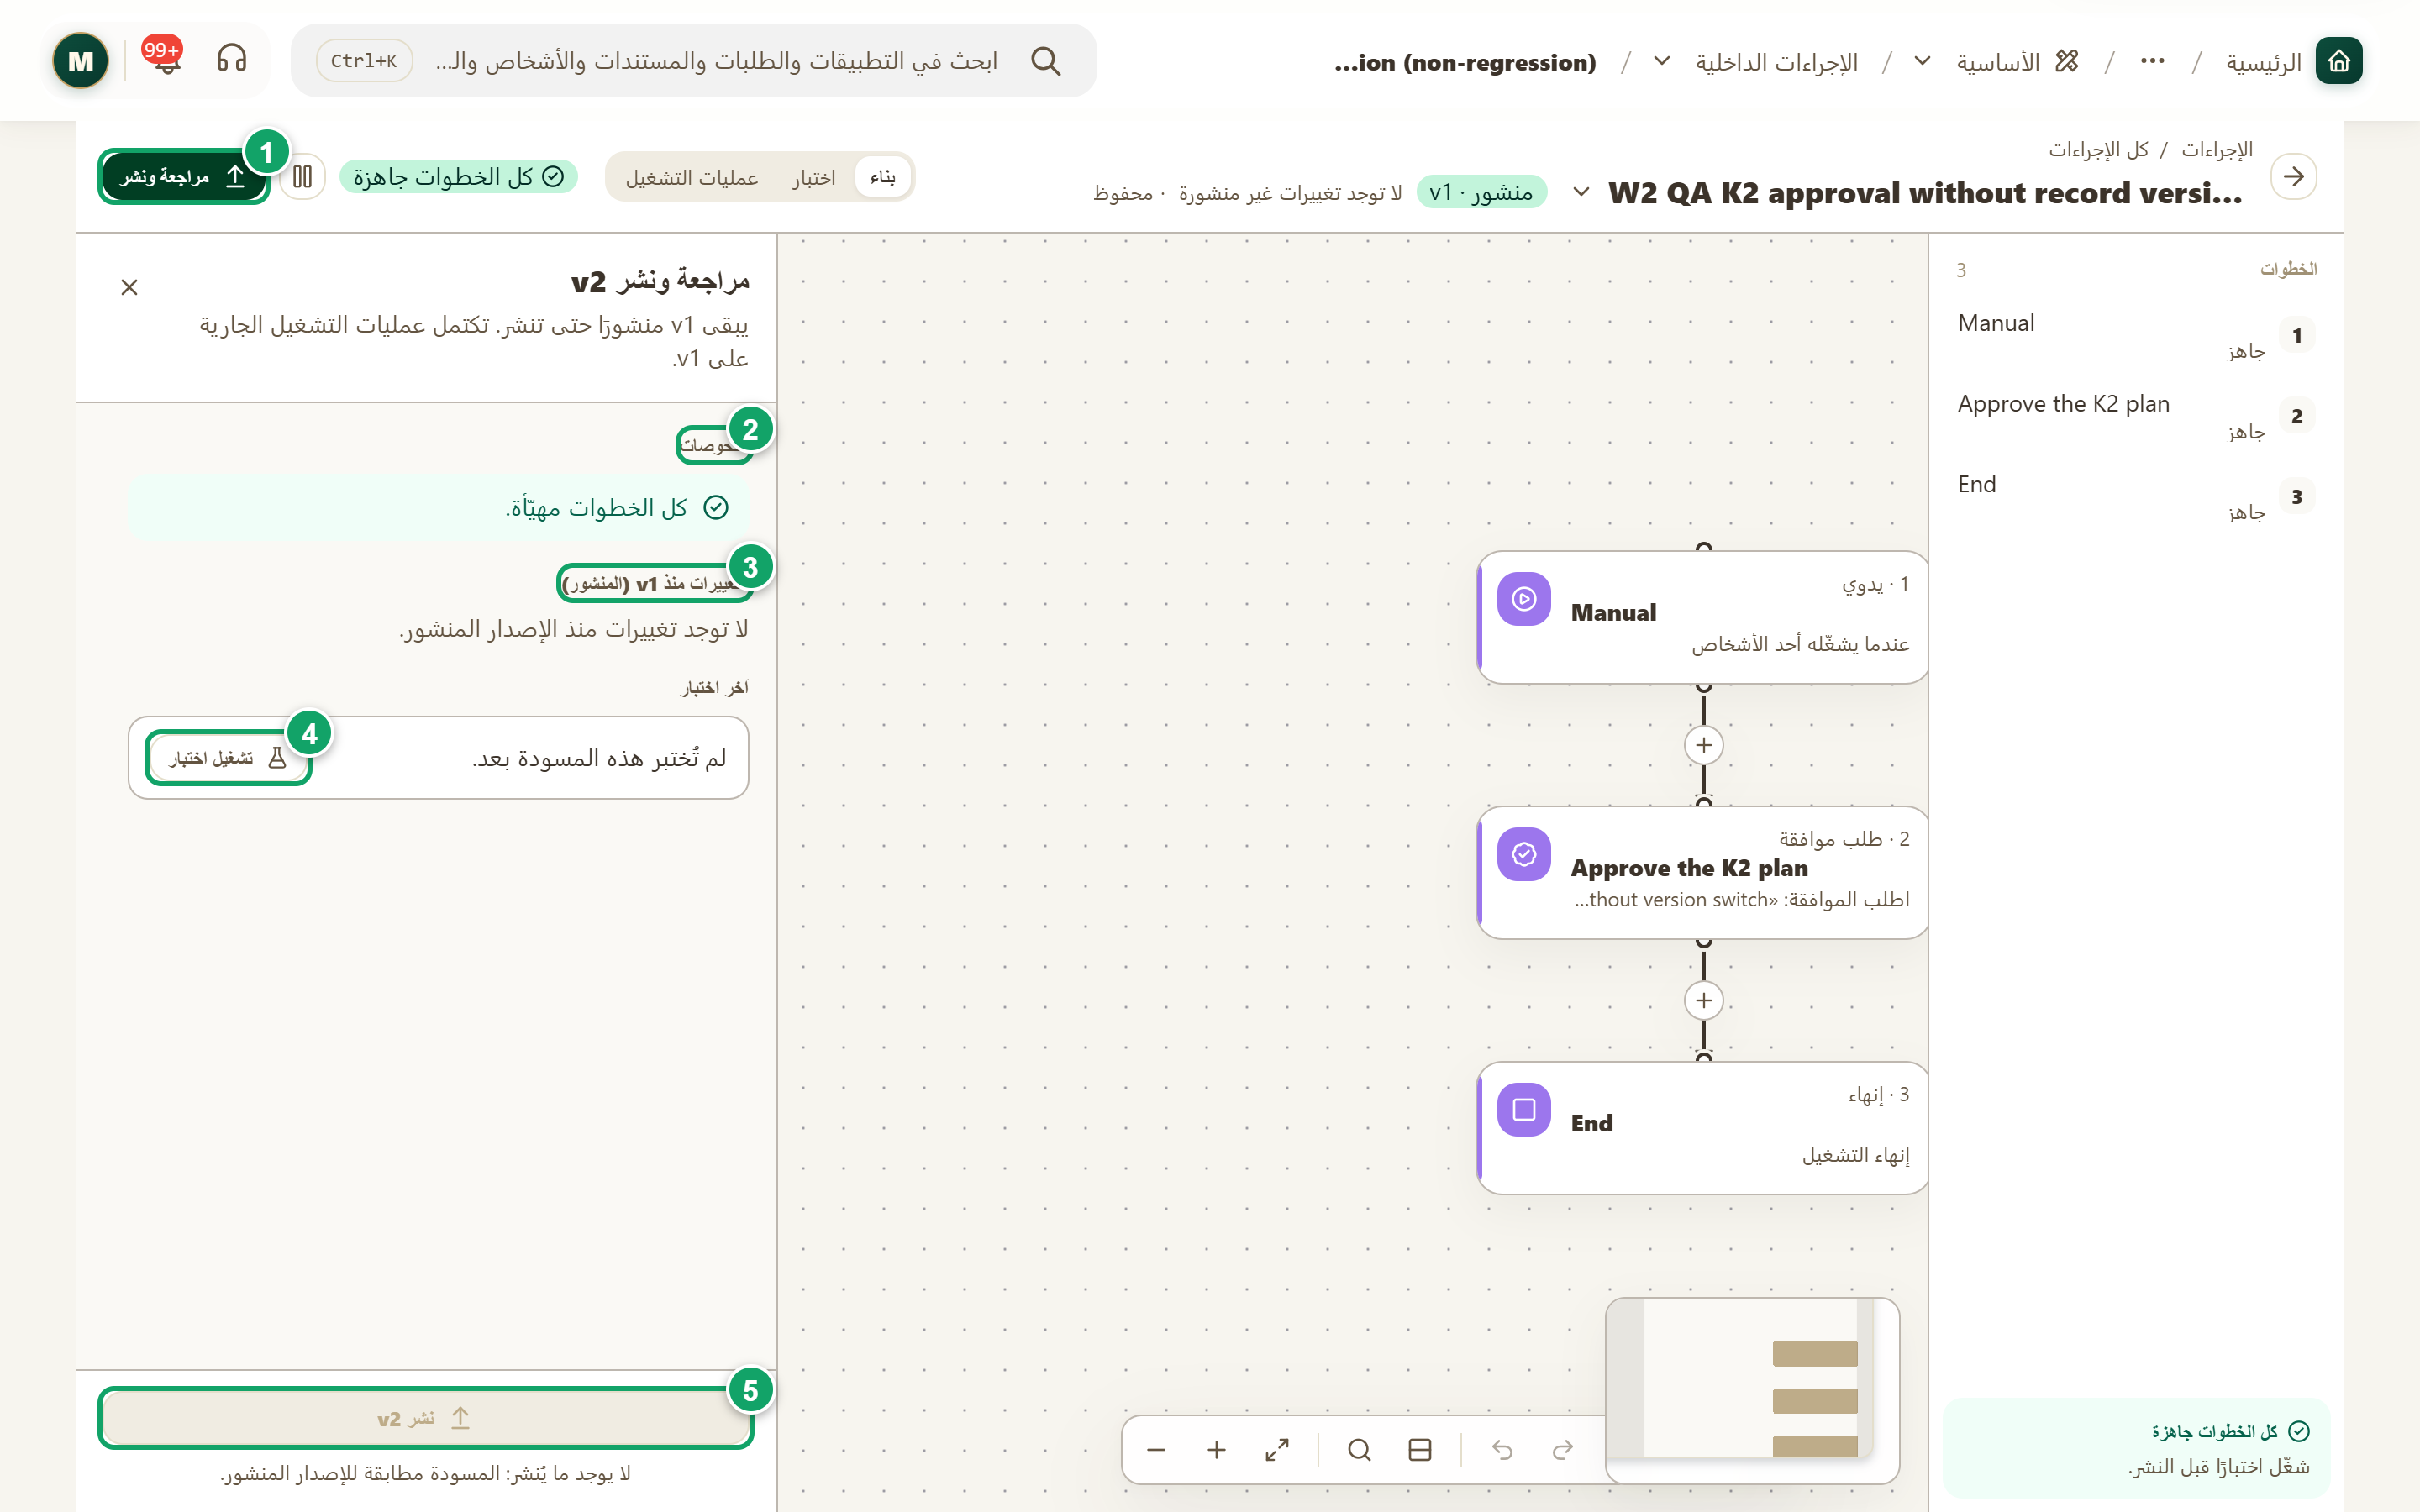
\includegraphics[width=0.95\linewidth,height=0.72\textheight,keepaspectratio]{figures/screens/ch06-isop-publish-ar.png}
\caption{لوحة «مراجعة ونشر v2» لإجراء منشور بلا تغييرات}
\label{fig:builder-isop-publish-screen}
\shotnote{تعرض الصورة لوحة المراجعة لإجراء منشور لم تتغير مسودته منذ \en{v1}، لذلك زر النشر معطّل وتحته سبب التعطيل. ولم يُنشر أي شيء عند الالتقاط؛ فاللوحة تبيّن ما تراجعه قبل النشر. ① «مراجعة ونشر»: يفتح اللوحة. ② «الفحوصات»: المشكلات التي تمنع النشر، أو تأكيد أن كل الخطوات مهيّأة. ③ «التغييرات منذ v1 (المنشور)»: ما تغيّر عن الإصدار المنشور. ④ «تشغيل اختبار»: يختبر المسودة قبل النشر. ⑤ «نشر v2»: ينشر الإصدار الجديد.}
\end{figure}

\begin{figure}[H]
\centering
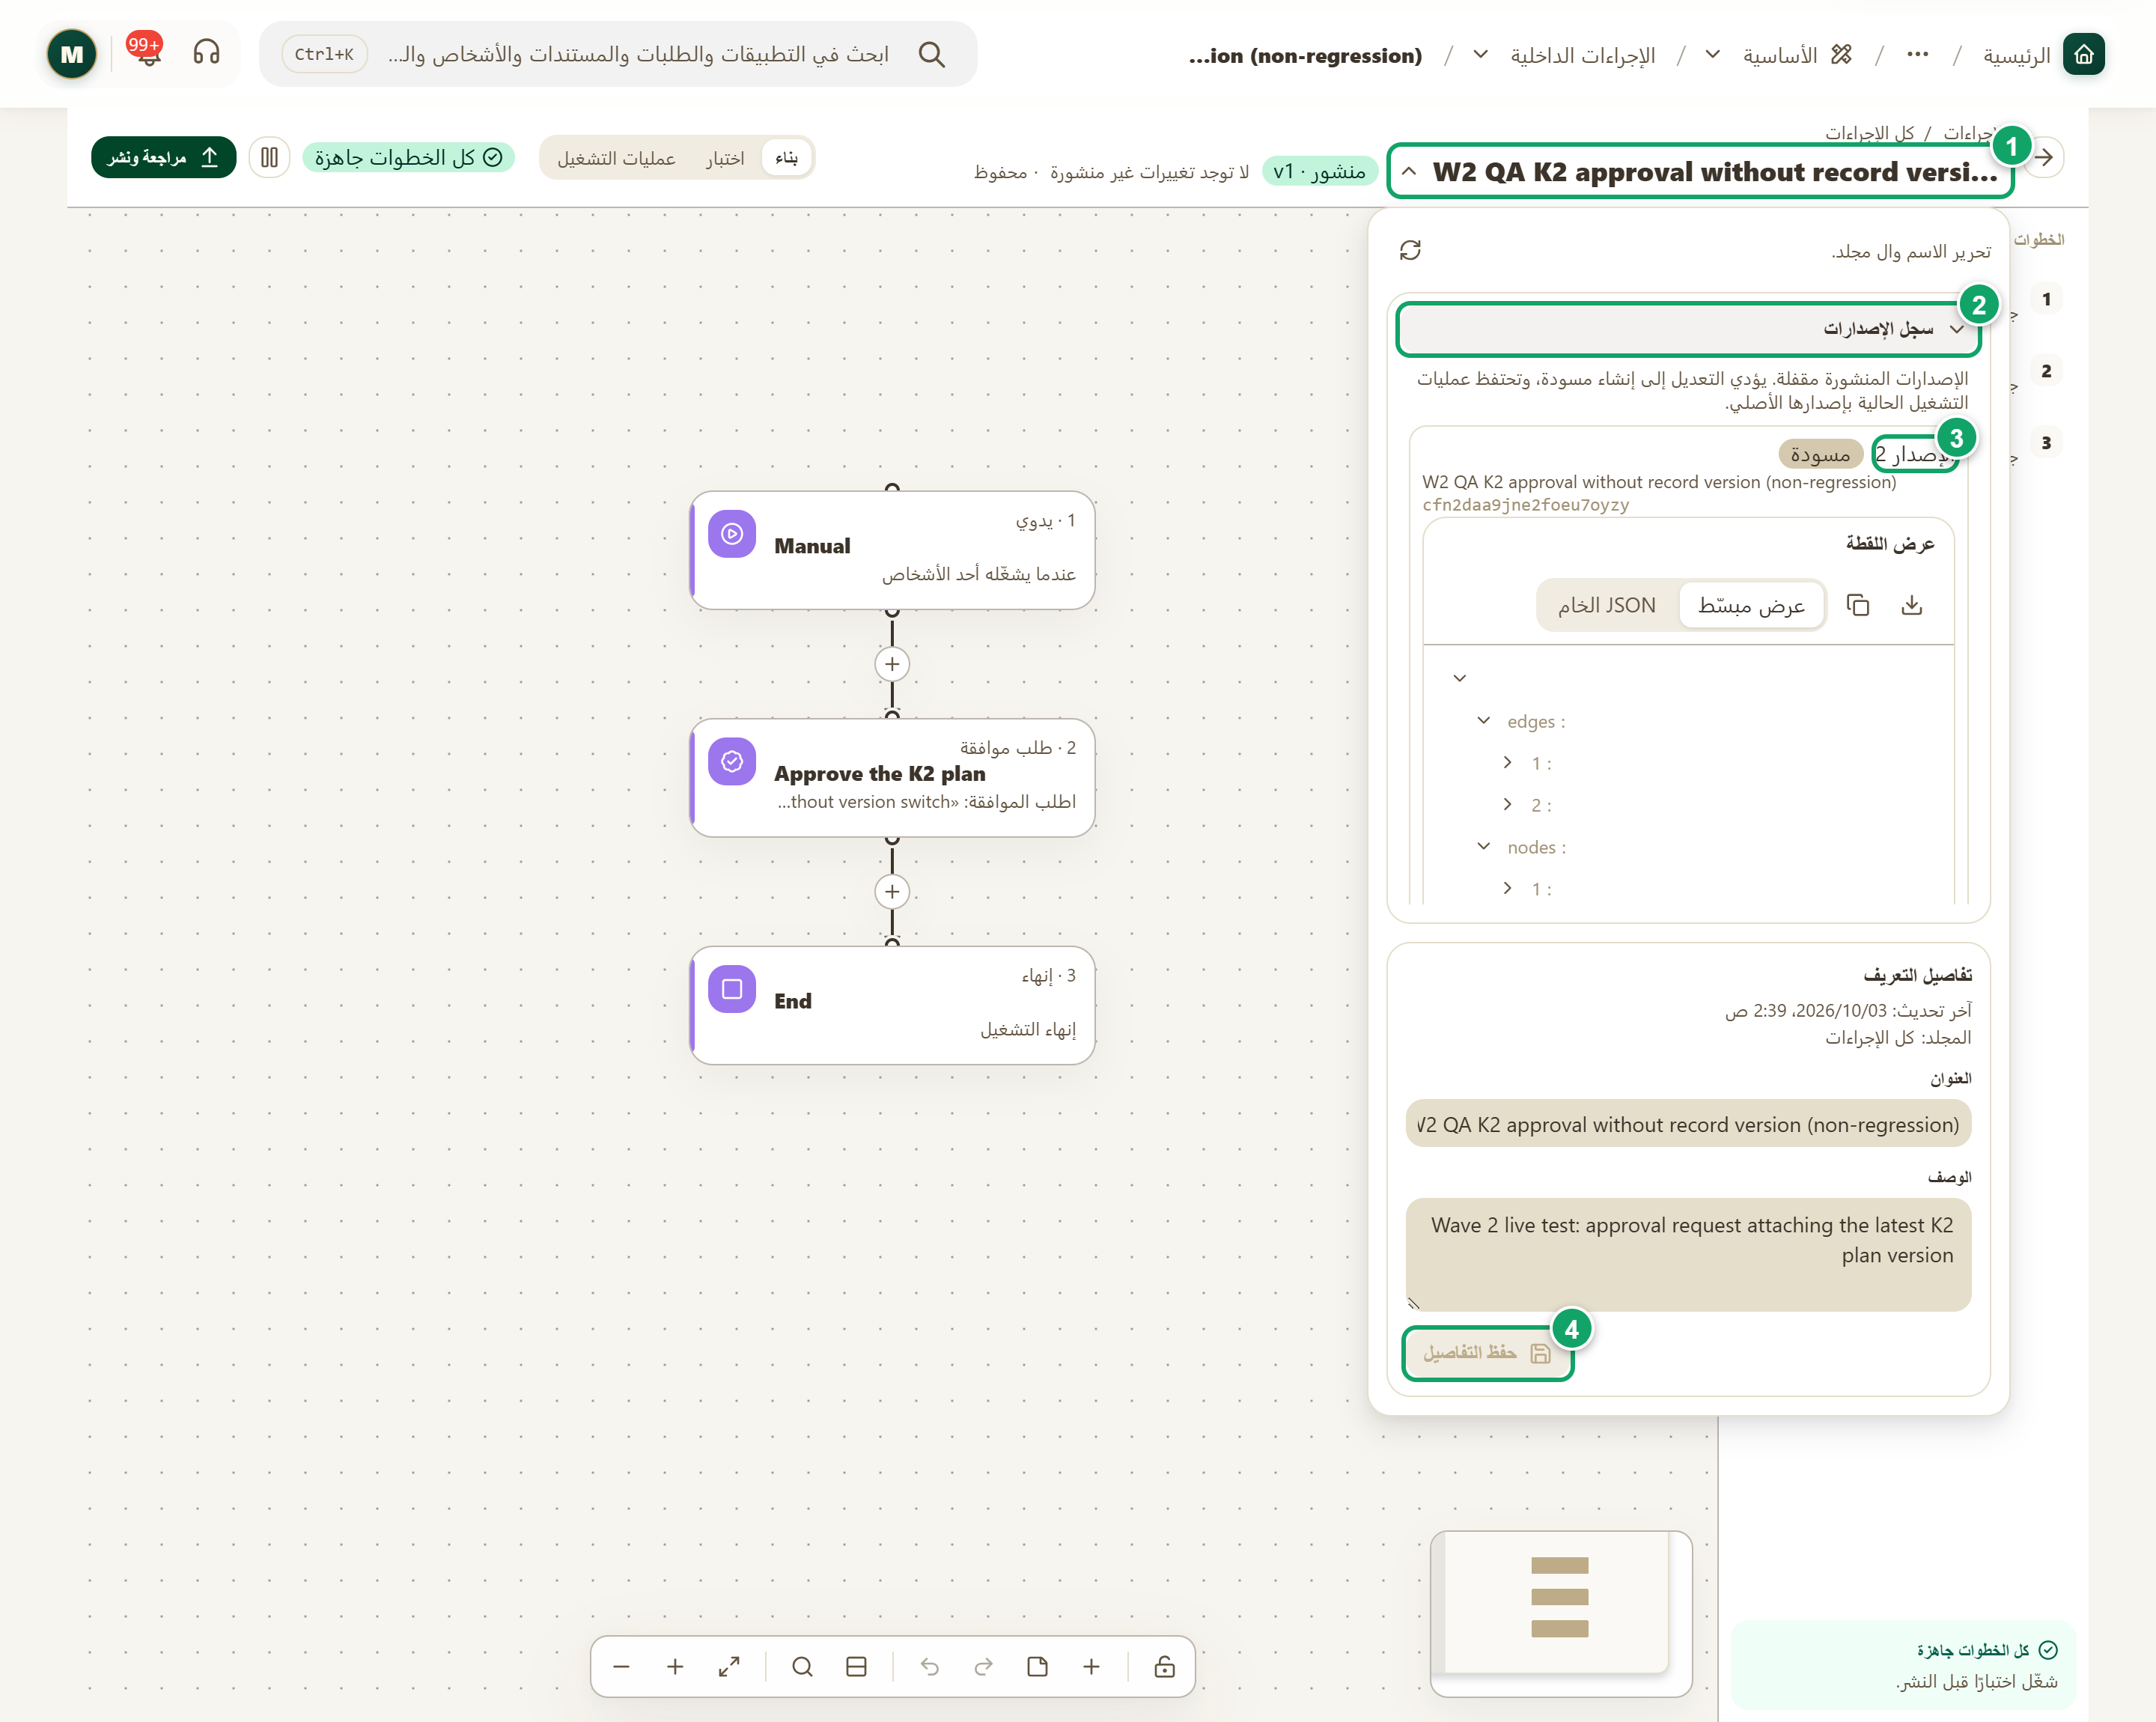
\includegraphics[width=0.95\linewidth,height=0.72\textheight,keepaspectratio]{figures/screens/ch06-isop-versions-ar.png}
\caption{سجل الإصدارات وتفاصيل التعريف}
\label{fig:builder-isop-publish-versions-screen}
\shotnote{تعرض الصورة القائمة التي تفتح من اسم الإجراء في رأس المحرر، وقد فُتح فيها «سجل الإصدارات» على المسودة الحالية مع لقطة تعريفها. وتذكّرك العبارة أعلى السجل بأن الإصدارات المنشورة مقفلة وأن التشغيل الجاري يبقى على إصداره. ① اسم الإجراء: يفتح هذه القائمة. ② «سجل الإصدارات»: يعرض الإصدارات ولقطاتها. ③ «الإصدار 2»: إصدار في السجل، وهو هنا مسودة. ④ «حفظ التفاصيل»: يحفظ العنوان والوصف بعد تعديلهما.}
\end{figure}

\begin{table}[H]
\centering
\caption{أقسام نافذة المراجعة}
\label{tab:builder-isop-publish-review}
\begin{tabularx}{\linewidth}{R{3.6cm} Y}
\rcHeaderRow
\thh{القسم} & \thh{ما يعرضه}\\
يجب إصلاحه قبل النشر & المشكلات التي تمنع النشر، ولكل منها زر «إصلاح» يفتح الخطوة. وعند خلوها يحمل القسم عنوان «الفحوصات» ويظهر فيه «كل الخطوات مهيّأة».\\
التغييرات منذ الإصدار المنشور & كل خطوة «مُضاف» أو «محذوف» أو «أُعيدت تسميته» أو «مُعدَّل»، وتغيّر «المسارات» بين الخطوات.\\
آخر اختبار & «نجح آخر اختبار لهذه المسودة» أو فشله أو «لم تُختبر هذه المسودة بعد»، مع «تشغيل اختبار». ويمكنك النشر دون اختبار، لكن الاختبار مستحسن.\\
زر النشر & «نشر \en{vN}». ويتعطل إذا بقيت مشكلات، أو كان الخادم غير متصل، أو لم يكن هناك ما يُنشر.\\
\end{tabularx}
\end{table}

\begin{table}[H]
\centering
\caption{بعد النشر}
\label{tab:builder-isop-publish-after}
\begin{tabularx}{\linewidth}{R{3.6cm} Y}
\rcHeaderRow
\thh{الأداة} & \thh{ما تفعله}\\
سجل الإصدارات & يعرض الإصدارات المنشورة المقفلة، ولكل منها «عرض اللقطة». والتعديل بعد النشر يُنشئ مسودة جديدة.\\
إيقاف الإجراء مؤقتًا & يمنع المشغّلات من بدء عمليات جديدة حتى «استئناف»، دون أن يحذف الإجراء أو إصداراته.\\
تفاصيل التعريف & تعدّل «العنوان» و«الوصف» ثم تضغط «حفظ التفاصيل».\\
\end{tabularx}
\end{table}

\begin{figure}[H]
\centering
\begin{tikzpicture}[node distance=0.5cm]
\node[stepBox] (a) {\RL{مسودة مكتملة}};
\node[stepBox,below=of a] (b) {\RL{مراجعة ونشر}};
\node[stepBox,below=of b] (c) {\RL{إصلاح المشكلات}};
\node[stepBox,below=of c] (d) {\RL{نشر الإصدار}};
\node[stepBox,below=of d] (e) {\RL{إصدار مقفل في السجل}};
\draw[flowsTo] (a) -- (b);
\draw[flowsTo] (b) -- (c);
\draw[flowsTo] (c) -- (d);
\draw[flowsTo] (d) -- (e);
\end{tikzpicture}
\rclegend
\caption{من المسودة إلى إصدار منشور}
\label{fig:builder-isop-publish-flow}
\shotnote{يبيّن المخطط أن كل نشر يُنتج إصداراً مقفلاً جديداً بدلاً من تعديل الإصدار السابق. لذلك لا يتأثر تشغيل بدأ قبل النشر، وتستطيع دائماً أن تعرف الإصدار الذي عمل عليه كل تشغيل.}
\end{figure}

\subsection{خطوات العمل والتحقق}
\begin{enumerate}
\item اضغط «مراجعة ونشر» في رأس المحرر.
\item اضغط «إصلاح» بجانب كل مشكلة، وأصلح الخطوة، ثم عُد إلى المراجعة.
\item راجع «التغييرات منذ» الإصدار المنشور، وشغّل اختباراً إن لم تختبر المسودة.
\item اضغط «نشر \en{vN}».
\item لمراجعة إصدار سابق، اضغط اسم الإجراء في رأس المحرر وافتح «سجل الإصدارات».
\end{enumerate}

\textbf{تحقق ومعالجة المشكلة:} يجب أن تظهر رسالة «أصبح \en{vN} منشورًا»، وأن تتغير شارة الإصدار إلى «منشور · \en{vN}». فإذا ظهر «لا يوجد ما يُنشر: المسودة مطابقة للإصدار المنشور»، فلم تغيّر شيئاً منذ آخر نشر. وإذا ظهر «تغيّرت المسودة أثناء النشر»، فانشر مرة أخرى لتشمل آخر تعديلاتك.
